\documentclass[11pt, a4paper]{report}
%-----------NORSK LaTeX--------------

% Denne pakken inkluderer skandinaviske bokstaver( æ, ø og å)
\usepackage[utf8]{inputenc}

% Denne pakken bruker norsk typesetting (innholdsliste osv.)
\usepackage[norsk]{babel}

%--------DOKUMENTOPPSETT------------

% Lar deg tilpasse layouten i prosjektet
\usepackage{fancyhdr}

% VIDEO?
\usepackage{media9}

% Definere egne farger 
\usepackage[usenames, dvipsnames]{color}

% Avstand på marger til sidene på arket
%\usepackage{geometry}

% Linker i dokumentet (figurer, seksjoner osv)
\usepackage[hidelinks]{hyperref}

% Kildeliste-setup
%\usepackage[natbibapa]{apacite} % For apalike eller apacite
\usepackage{natbib} % For Chicago, Vancover, Harvard Style, Nature Style osv

% Spacing mellom bokstaver
\usepackage{microtype}

% Laster inn forskjellige skrifttyper
\usepackage{uarial} % Arial
\usepackage[scaled]{helvet} % Helvetica
%\usepackage{tgbonum} % Usikker
%\usepackage{mathptmx} % Times New Roman
%\usepackage{lmodern} % Latin Modern
%\usepackage[charter]{mathdesign} % Charters
\usepackage[T1]{fontenc}

% Avsnitt mellom paragrafer
\usepackage{parskip}

% Linjeavstand i dokumentet
\usepackage{setspace}
\setlength{\parskip}{1em}

% Fet skrift på alle figurnr
\usepackage[labelfont=bf]{caption}
\usepackage{capt-of}
\usepackage{caption}
\usepackage{tikz}

\usepackage{chngcntr}
\counterwithin{figure}{chapter}
\counterwithin{table}{chapter}

% Definerer mellomrom mellom seksjons-, figur- og tabellnummer i innholdsliste til teksten begynner
\renewcommand{\numberline}[1]{#1 \,}

% Kan skrive i kolonner
\usepackage{multicol}

% For appendix
\usepackage{titletoc}
\usepackage{appendix}

%----------ANDRE PAKKER--------------

% Pakker fra AMS. Kan skrive matteformler
\usepackage{amsfonts, amssymb, amsthm}
\usepackage{mathtools}

% For grafikk (lime inn bilder, pdf-dokumenter)
\usepackage{graphicx}
\usepackage{float}
\usepackage{pdfpages}
\usepackage{subcaption}

% For inportering av csv-filer som tabeller. ( Ikkje i bruk)
%usepackage{csvsimple}

% Pakke for citations
%\usepackage{biblatex}
% Pakke for at url linker skal fungere i bl.a. referansar
\usepackage{url}

% Generere tekst
\usepackage{kantlipsum}

% Definere egne objekt
\usepackage{tikz}

% Lar deg lage lister på en mer oversiktlig måte
\usepackage[sharp]{easylist}

% Boks rundt tekst
\usepackage{fancyvrb}

% Test pakker
\usepackage{array}
\usepackage[margin=1in]{geometry} % Juster margene etter behov
\usepackage{titlesec}
\usepackage{tabularx}
\usepackage[table]{xcolor}
\usepackage{lastpage}

% pakke for ordliste
\usepackage[automake]{glossaries-extra}

% For å kunne justere bilete
\usepackage{adjustbox}

% 
\usepackage{tocloft}


% Sider til SCD
\usepackage{afterpage}
\usepackage{adjustbox}


\usepackage{etoolbox} % For å koble kommandoer
%---------------------------------------------------

% Legger til bookmarks i pdf
\hypersetup{
    bookmarks=true, % Aktiver bokmerker
    bookmarksnumbered=true, % Inkluder nummer i bokmerker
    pdfstartview={FitH}, % Åpner PDF med passende bredde
    %colorlinks=true, % Farger lenker i stedet for å bruke bokser
    %linkcolor=blue, % Intern lenkefarge
    %filecolor=magenta, % Fil-lenkefarge
    %urlcolor=cyan % URL-lenkefarge
}



% Velger arial som skrifttype i dokumentet 
%\renewcommand{\rmdefault}{qpl} % 
%\renewcommand{\rmdefault}{phv} % Arial
\renewcommand*\familydefault{\sfdefault} % Helvetica(sans-serif)


% Definerer egne farger
\definecolor{mybla}{RGB}{25, 49, 90}
\definecolor{mylysbla}{RGB}{0, 136, 176}
\definecolor{renasysGreen}{RGB}{4, 255, 4}
\definecolor{purewhite}{RGB}{255,255,255}
\definecolor{lightgray}{gray}{0.8}
\definecolor{myblack}{gray}{0.1}

% Velger norsk språk på innholdsfortegnelse, figurliste, tabelliste og Referanseliste
% Legger disse så til i innholdsfortegnelsen.
\addto\captionsnorsk{\renewcommand{\contentsname}{Innhaldsliste}}
\addto\captionsnorsk{\renewcommand{\listfigurename}{Figurliste}}
\addto\captionsnorsk{\renewcommand{\listtablename}{Tabelliste}}
\addto\captionsnorsk{\renewcommand{\bibname}{Referansar}}
% Nynorsk!
\addto\captionsnynorsk{\renewcommand{\contentsname}{Innhaldsliste}} 
\addto\captionsnynorsk{\renewcommand{\listfigurename}{Figurliste}}
\addto\captionsnynorsk{\renewcommand{\listtablename}{Tabelliste}}
\addto\captionsnynorsk{\renewcommand{\bibname}{Referansar}}


% ----- Justering av avstander mellom chapter / section / subsection / subsubsection

% Justeringa av chapter, 
% første verdi : Horisontalverdi frå venstre marg
% Andre verdi : avstanden frå toppen av sida til tittelen
% Tredje verdi : Avstand til neste tekst
\titleformat{\chapter}[hang]
  {\normalfont\bfseries\LARGE}{\thechapter}{1em}{}
\titlespacing*{\chapter}{0pt}{-50pt}{0pt}

% Juster avstanden for \section
\titleformat{\section}
  {\normalfont\Large\bfseries}{\thesection}{1em}{}
\titlespacing*{\section}{0pt}{10pt}{10pt}

% Juster avstanden for \subsection
\titleformat{\subsection}
  {\normalfont\large\bfseries}{\thesubsection}{1em}{}
\titlespacing*{\subsection}{0pt}{10pt}{10pt}

% Juster avstanden for \subsubsection om nødvendig
\titleformat{\subsubsection}
  {\normalfont\normalsize\bfseries}{\thesubsubsection}{1em}{}
\titlespacing*{\subsubsection}{0pt}{10pt}{10pt}

% ------------------- jusetring av lister ------------------

% Denne vil endre skriftstørrelse ...
% Legg til \hfill før LARGE om overskrifta skal sentrerest
\renewcommand{\cfttoctitlefont}{\LARGE\bfseries}
\renewcommand{\cftaftertoctitle}{}
\renewcommand{\cftloftitlefont}{\LARGE\bfseries}
\renewcommand{\cftafterloftitle}{}
\renewcommand{\cftlottitlefont}{\LARGE\bfseries}
\renewcommand{\cftafterlottitle}{}

% Avstand mellom toppen av sida og ned til overskrifta t.d. innhaldsliste
\setlength{\cftbeforetoctitleskip}{-20pt}  % Adjust the value as needed, negative reduces the space
\setlength{\cftbeforeloftitleskip}{-20pt}  % Adjust the value as needed
\setlength{\cftbeforelottitleskip}{-20pt}  % Adjust the value as needed

% Avstand mellom Overskrift og kapittel
\setlength{\cftaftertoctitleskip}{15pt}
\setlength{\cftafterloftitleskip}{15pt}
\setlength{\cftafterloftitleskip}{15pt}


% -------------------------------------------------------------

% Her definerer ein pagestylen til hovud opplegget
\fancypagestyle{fancy}{
  % Clear the header and footer
  \fancyhf{}
  % Set the right side of the footer to be the location of the page number
  \fancyfoot[R]{Side \thepage\ av~\pageref{LastPage}} % Her sett ein fra side til side
  \renewcommand{\headrulewidth}{0pt} % Remove header line
  \renewcommand{\footrulewidth}{0pt} % Remove footer line
}

% Her definerer ein pagestylen til dei sidene som skal ha romartall
\fancypagestyle{romanpages}{
  % Clear the header and footer
  \fancyhf{}
  % Set the right side of the footer to be the location of the page number
  \fancyfoot[R]{\thepage}
  \renewcommand{\headrulewidth}{0pt} % Remove header line
  \renewcommand{\footrulewidth}{0pt} % Remove footer line
}


% ------ Justering av avstander i dokumentet for itemize ---------------------

\let\olditemize\itemize
\renewcommand{\itemize}{
  \olditemize
  \setlength{\itemsep}{-10pt} 
}

% ------ Justering av avstander i dokumentet for enumerable ---------------------

% Save the original definition of enumerate
\let\oldenumerate\enumerate

% Redefine the enumerate to adjust spacing
\renewcommand{\enumerate}{
  \oldenumerate
  \setlength{\itemsep}{-7pt}  % Adjust this value as needed
}

% -------------------------------------------------------------------



% ------------------------- KODE FOR ORDLISTE ---------------------

% Kode for å lage ei meir kompakt ordliste
\newglossarystyle{compact}{%
  % base this style on the list style:
  \setglossarystyle{list}%
  % adjust the space between entries:
  \renewenvironment{theglossary}{%
    \begin{description}%
    \setlength{\itemsep}{-10pt}% adjust this value as needed
    \setlength{\parskip}{0pt}%
  }%
  {%
    \end{description}%
  }%
}

\setglossarystyle{compact}

% Kode for å lage stil for ordlista
\newglossarystyle{tablestyle}{
  % Start the glossary as a tabular environment
  \renewenvironment{theglossary}{
	\setlength{\LTleft}{0pt} % Align the table with the left margin
    \begin{longtable}{lp{\glsdescwidth}}
    }{
    \end{longtable}
  }
  \renewcommand*{\glossaryheader}{
    \bfseries Term & \bfseries Forklaring \\
    \endfirsthead
    \bfseries Term & \bfseries Forklaring \\
    \endhead
  }
  % No heading between groups
  \renewcommand*{\glsgroupheading}[1]{}
  % No space between groups
  \renewcommand*{\glsgroupskip}{}
  % Define how each entry should appear:
  \renewcommand*{\glossentry}[2]{
    \glstarget{##1}{\glossentryname{##1}} &
    \glossentrydesc{##1} \\
  }
}

% Setter Stil for Ordlista
\setglossarystyle{tablestyle}


\makeglossaries
\loadglsentries{Ordliste.tex}

% Stil for referansar
\bibliographystyle{unsrt}

% Endre namn på overskrifta til referanselista

% dette må stå her slik at romartalla viser korrekt i rapporten
\makeatletter
\let\ps@oldplain\ps@plain
\renewcommand\ps@plain{\pagestyle{romanpages}}
\makeatother


% ---------------------------------- END kode for ordliste -----------------------------

% ------------------------------------ Dokumentet starter her ----------------------------

\begin{document} % Dokument start



	%------------------FREMSIDE------------------------

	% Linker inn fremsiden fra adms (administrative sider) fremside-filen.
	% Førstesiden skal ha følgende marger.
\newgeometry{top=2.5cm,bottom=2.5cm,right=3cm,left=5cm}

% Ønsker ikke sidetall på denne siden.
\thispagestyle{empty}


% Legger inn banner
\begin{center}
	\begin{tikzpicture}[remember picture, overlay]
	\node [xshift=0cm, yshift=11.5cm] at (current page.center) 
	{
\includegraphics[width=\paperwidth]{Bilder/framsideNynorsk.png}};
	\end{tikzpicture}
\end{center}



\vspace{6cm}

{\fontsize{36}{50}\selectfont \textbf{\textcolor{mybla}{BACHELOROPPGÅVE}}} 
\newline
\newline
{\fontsize{26}{30}\selectfont \textcolor{mybla}{RA200 Sande}}

\vspace{1cm}
% Forfattarar
{\fontsize{26}{30}\selectfont \textbf{\textcolor{mylysbla}{Roar Bøyum}}}\\
{\fontsize{26}{30}\selectfont \textbf{\textcolor{mylysbla}{Vegard Aven Ullebø}}}\\
{\fontsize{26}{30}\selectfont \textbf{\textcolor{mylysbla}{Peter Søreide Skaar}}}\\ 


\vspace{1.3cm}


\setstretch{0.7}

{\fontsize{20}{20}\selectfont\textcolor{mylysbla}{Automatisering med robotikk}} 

\vspace{-0.4cm}
{\fontsize{20}{20}\selectfont\textcolor{mylysbla}{Fakultet/Institutt/program}} 

\vspace{-0.4cm}
{\fontsize{20}{20}\selectfont\textcolor{mylysbla}{Rettleiarar: Olav Sande, Joar Sande og \newline Bjarte Pollen}} 

\vspace{-0.4cm}
{\fontsize{20}{20}\selectfont\textcolor{mylysbla}{Innleveringsdato: 21.05.2024}} 



% Endrer skriften for resten av dokumentet
{\fontfamily{qpl}\selectfont}


\vspace{1cm}

\setstretch{0.8}
{\fontsize{9.5}{20}\selectfont
Eg stadfestar at arbeidet er sjølvstendig utarbeida, og at referansar/kjeldetilvisingar til alle
kjelder som er brukt i arbeidet er oppgitt, jf. Forskrift om studium og eksamen ved Høgskulen på Vestlandet, § 12-1.
}
	

	%------------------------------------------------------

	\newpage

	% Nye marger
	\newgeometry{top=2.5cm,bottom=3cm,right=2.2cm,left=2.2cm}

	% Linjeavstand
	\setstretch{1.3}

	% Set the right side of the footer to be location of the page number

	% Ønsker tallnummerering videre.
	%-------------------- 			FORORD / Samandrag			---------------------	
	\pagenumbering{Roman}
	\setcounter{page}{2}
	\chapter*{}
\thispagestyle{romanpages}

% Sentrere bildet helt nøyaktig på siden
\noindent\begin{adjustbox}{center=\paperwidth}
	\hspace*{-0.25\textwidth} % justering venstre høgre på bilde
    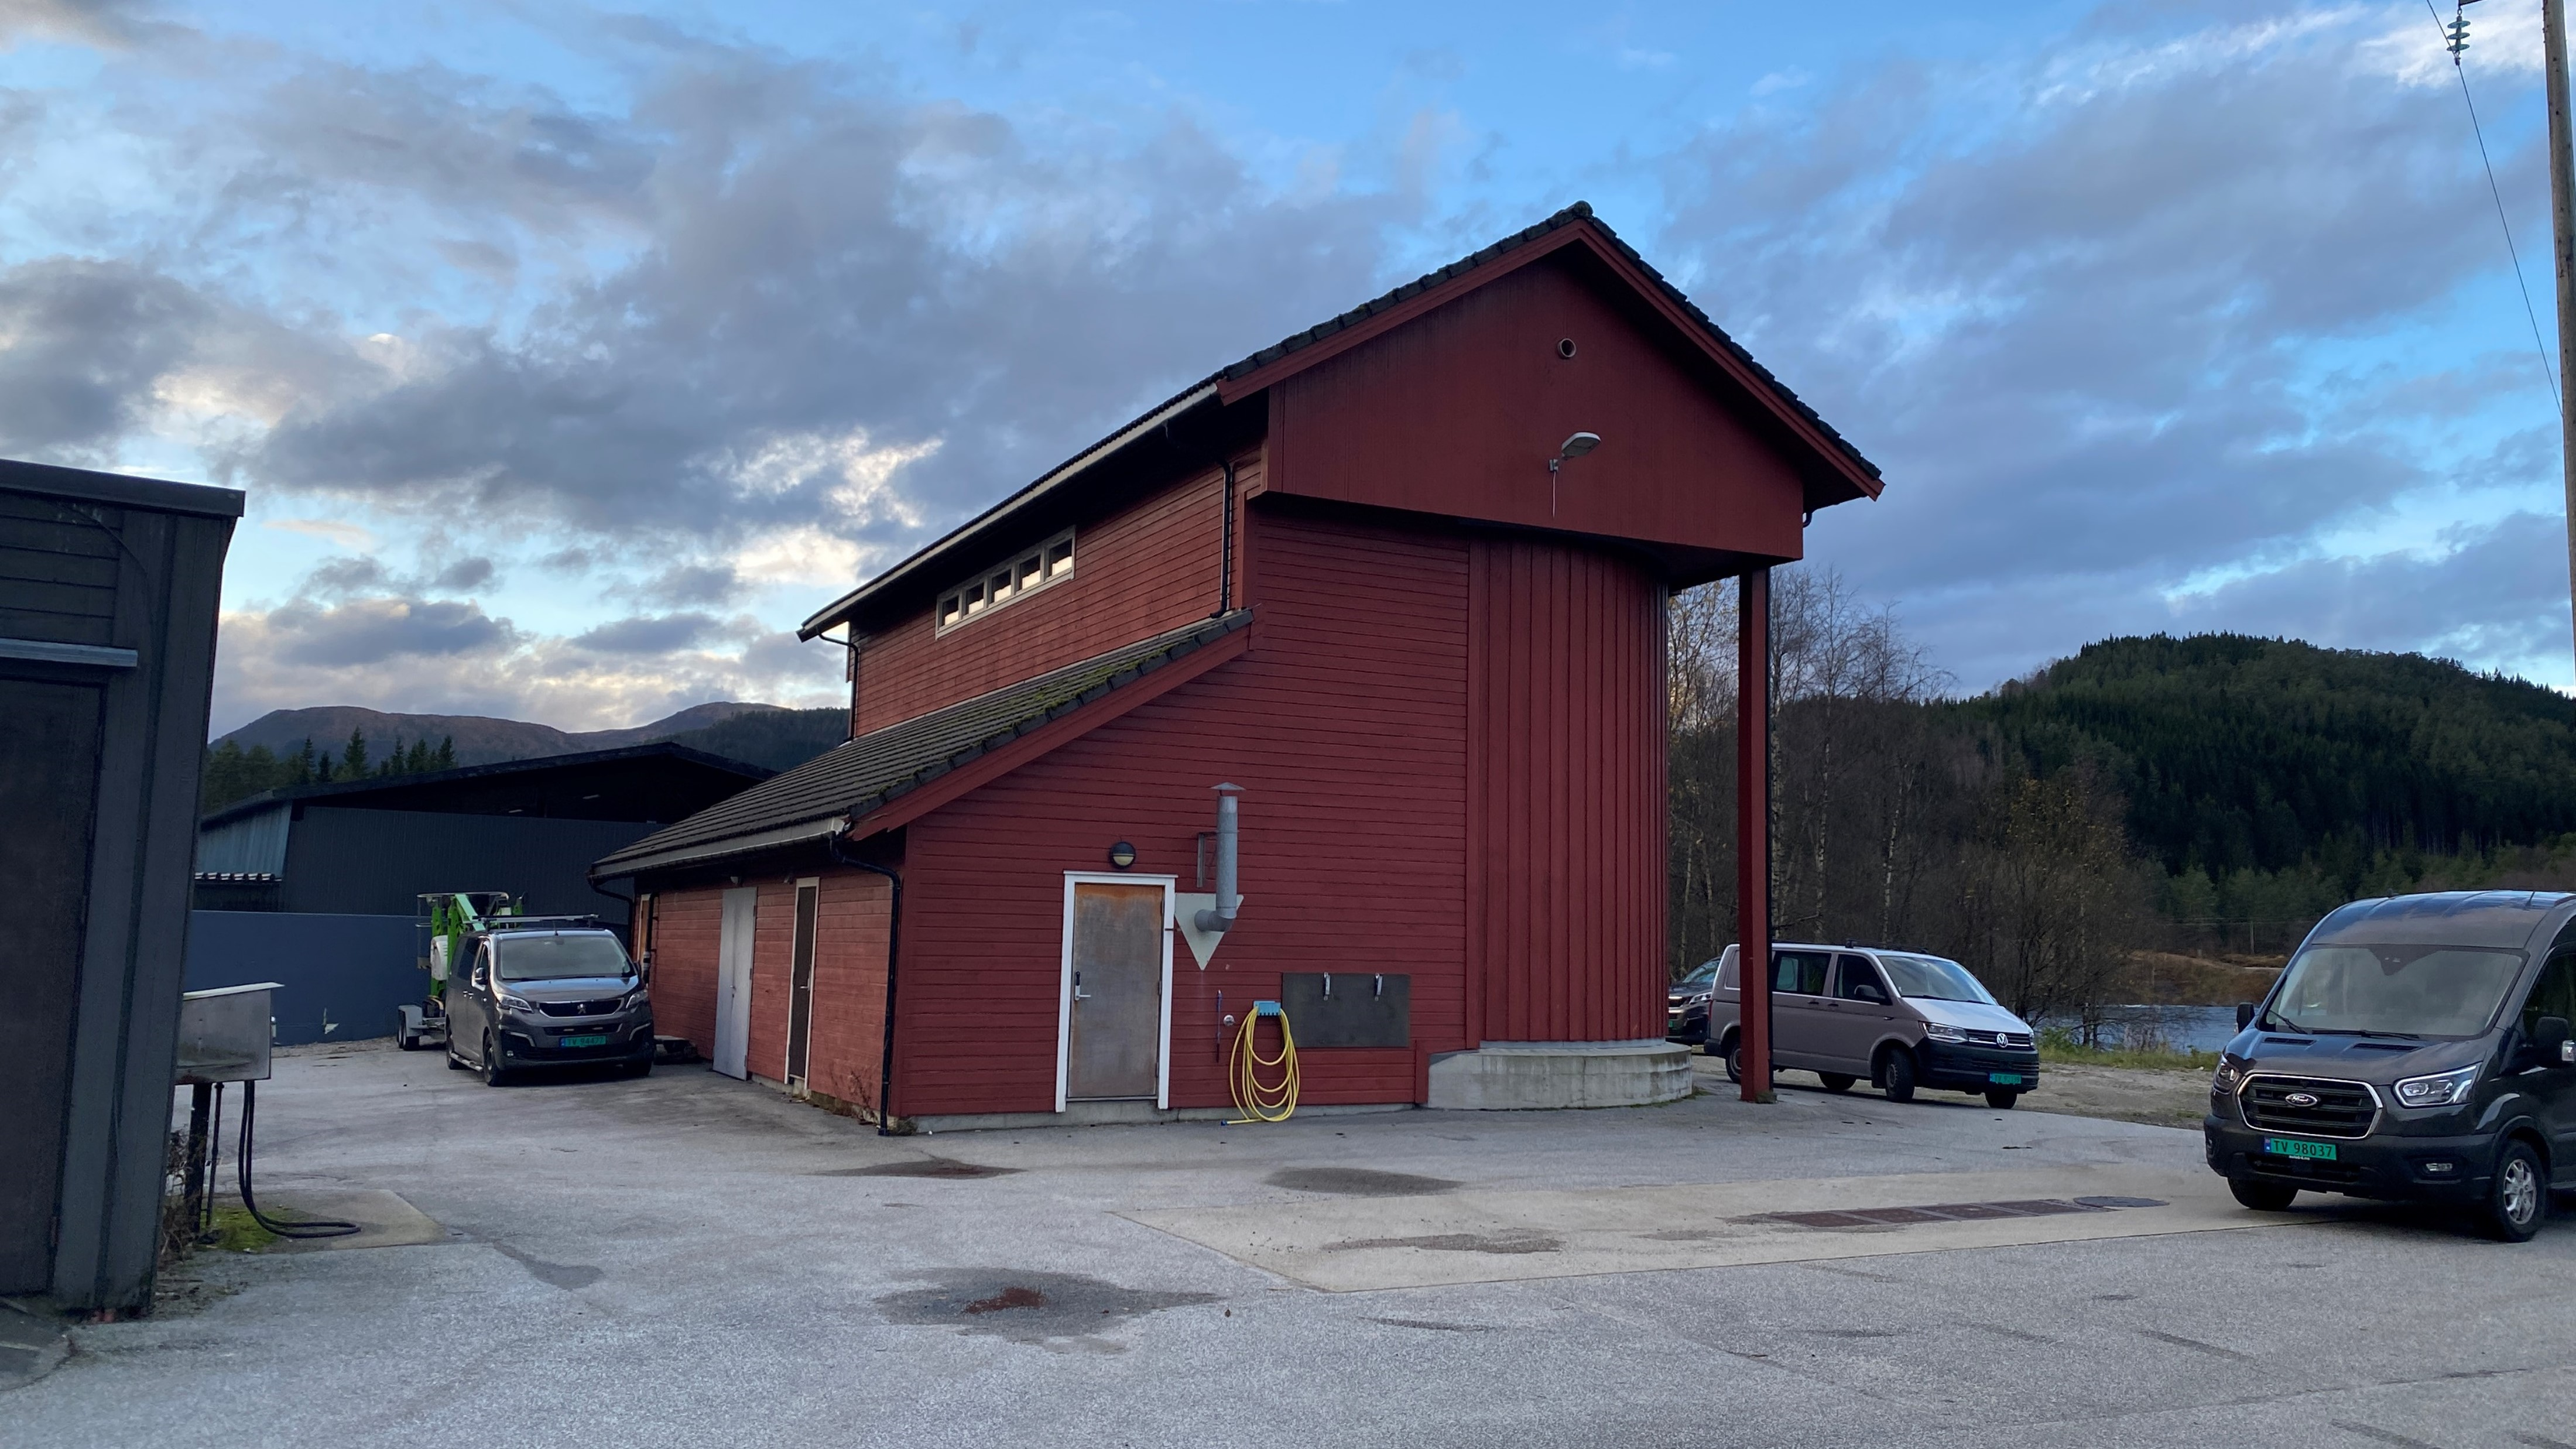
\includegraphics[width=1.1\textwidth]{Bilder/Framside RA200.jpg}
\end{adjustbox}

	\chapter{Forord}
\thispagestyle{romanpages}


Denne rapporten er skreven på vegne av \gls{Renasys}\citep{Renasys} og \gls{Sunnfjord Kommune}\citep{SunnfjordKommune}, i emnet
ELE350-1 23H Bacheloroppgave. Vi starta prosjektet i Januar og er ferdig i slutten av mai.

-- Lage noko eige for takk?

Tusen takk til arbeidsgivarar Renasys og Sunnfjord kommune som har gjort denne oppgåve mogleg.
Tusen takk til alle som har hjelpt og bidratt til arbeidet med denne bacheloroppgåva og
takk til MidTechnolegies og HVL for aktuelle lisensar brukt i oppgåva.

Spesiell takk til familie og vennar som har støtta oss i denne prosessen.


% Bør innehalde
% - Hvorfor arbeidet ble utført
% - Personlige motivasjoner eller inspirasjoner for prosjektet
% - Hvordan prosjektet utviklet seg, eventuelle utfordringer underveis
% - eventuelle spesielle forhold eller omstendigheter rundt forskningen

-- Flytte introduksjon av oss hit ? \newline
-- Flyttes til appendix? All kode for denne bacheloroppgåva er samla i ein felles github (SETT INN LINK)

	\chapter{Samandrag}
\thispagestyle{romanpages}

Bacheloroppgåva, som vi har løyst i saman med \gls{Renasys} og \gls{Sunnfjord Kommune}, handlar om utbetring av styresystemet på 
avlaupsreinseanlegget i Sande i Sunnfjord. 
Anlegget er teknisk utdatert noko som gjer at oppgradering av styresystemet undersøkjast.

Rapporten legg til rette for fire ulike løysningsalternativ
der ulik grad av dybde blir presentert og vurdert. \newline
Rapporten legg til grunn val av løysningsalternativ C der alternativet bygger på planlegginga av eit nytt styresystem.
Rapporten undersøkjar og forklarer generell verkemåte til eit avlaupsreinseanlegg og 
vidare forklarer og dokumenterar reinseanlegget på Sande.

Oppgåva gir innblikk i dei relevante stega i planlegging av eit nytt styresystem der eigen dokumentasjon er brukt som grunnlag for vidare arbeid. 
Utføring av programmering, simulering og testing er løyst med eigne funskjonsblokker og metodar i programmeringsverktøyet \gls{Codesys},
der annerkjende \gls{IEC} standarar er undersøkt og tatt i bruk.
Vidare blir styresystemet og programmeringsarbeidet skildra og dokumentert.

Resultatet av bacheloroppgåva gir vår arbeidsgivar ny og forbetra dokumentasjon av anlegget 
og grunnlaget for eit nytt, fleksibelt og teknisk moderne program. 
Rapporten undersøkjer også generelle oppgraderingar og ytterligare forbetringspotensial 
for reinseanlegget og programmet.

	%--------------------Innhaldsliste / Figurliste / tabell liste---------------------	
	% innholdsliste
	\cleardoublepage
	\pagestyle{romanpages}
	\tableofcontents
	\thispagestyle{romanpages}  % Apply to the first page of the Table of Contents

	\cleardoublepage
	\pagestyle{romanpages}
	\listoffigures
	\thispagestyle{romanpages}  % Apply to the first page of the List of Figures
	
	%\cleardoublepage
	%\pagestyle{romanpages}
	%\listoftables
	\thispagestyle{romanpages}  % Apply to the first page of the List of Tables

	% Turn on the style
	\pagestyle{fancy}


	\clearpage
	\pagenumbering{arabic}
	%\setcounter{page}{5}

	%------------------------------------------------------

	%------------------ Lim inn sider til documentet her ------------------------



	% Kapittel 3 Innleiing
	\chapter{Innleiing}
\thispagestyle{fancy}

\section{Om oss}

Vi er tre studentar som studerar Automasjon med robotikk ved HVL campus Førde.
Vi har alle fagbrev som elektrikar og fant lett tonen i starten på studiet.
Igjennom tre år har vi brukt vår breie kompetanse innen industri, programmering og elektronikk
til å danne eit godt team.

Roar Bøyum har arbeidserfaring frå Kongsberg Maritim og Rolls Royce og er busatt i Sogndal.
Vegard Aven Ullebø har arbeid innan fleire industrifelt også offshore og er busatt i Vadheim i Høyanger.
Peter Søreide Skaar er busatt i Førde og har deltidsstilling i Renasys.



	\section{Oppdragsgivar}
\textbf{Renasys AS i samarbeid med Sunnfjord kommune}

Renays\citep{Renasys} kan skildrast som ein innovativ og nyskapande oppstarts bedrift som arbeider med banebrytande teknologi innan mekanisk finpartillekfiltering av avlaupsvatn.
Bedrifta har 14 tilsette fordelt på forskjellige lokasjonar, dei har kontor på Øyrane i Førde og Sandnes i Rogaland. 
Etter å ha arbeidd konfidensielt over lengre tid, gjekk Renasys offentleg ut med teknologien sin i løpet av 2023. 
Dei tilbyr også reinsetjenester til kommunar og interkommunale selskap innan avlaup og maritim sektor.

Samarbeidet med Sunnfjord kommune\citep{SunnfjordKommune} er retta mot 'Mission Zero' som er eit ambisiøst mål om 
null utslepp, null avfall, null energi og ein generell modernisering av avlaupssektoren i Norge.
Sunnfjord kommune er ansvarleg for vann, veg og avlaup i sitt område, har engasjert 
Renasys for å utforske forbetringar ved reinseanlegget på Sande.
\newline
\newline


\begin{figure}[htbp]
    \centering
    \begin{subfigure}[b]{0.3\textwidth}
        \centering
        
\includegraphics[width=1\textwidth]{Bilder/renasys.png}
    \end{subfigure}
    \hfill
    \begin{subfigure}[b]{0.3\textwidth}
        \centering
        
\includegraphics[width=0.7\textwidth]{Bilder/SK.png}
    \end{subfigure}
    \caption{Logo oppdragsgivar}\label{fig:Oppdragsgivar}
\end{figure}

	% Kapittel 4 Analyse av problemet
	\chapter{Analyse av oppgåva}
\thispagestyle{fancy}
Sande reinseanlegg ligg 25 minuttar med bil frå Førde sentrum og er ein 
av dei større reinseanlegga i \gls{Sunnfjord Kommune}. Anlegget er dimensjonert for 1500 personekvivalentar
og vart bygd i 2003. Anlegget har fleire utfordringar, og ein av desse utgjer ei problemstilling som egnar seg godt til ei
bacheloroppgåve innan automasjon.
	\section{Problemstilling}
Reinseanlegget er teknisk utdatert og treng fornying. Styresystemet, som no er over tjue år gammalt,
består hovudsakeleg av eldre og utgåtte komponentar. Med eldre komponentar aukar risikoen for svikt, 
og det kan vere vanskeleg å finne passande reservedelar.

WaterCare AS \citep{WaterCare}, som opphavleg leverte styresystemet har i seinare tid blitt avvikla. 
Dette gjer at kompetansen innan styresystemet og moglegheita for å gjere endringar i det, er utfordrande.
Grunna desse utfordringane har ikkje anlegget klart å halde tritt med den teknologiske utviklinga, 
og mindre problem har gradvis auka til større utfordringar.

Samstundes med desse faktorane er dokumentasjonen til reinseanlegget mangelfull, noko som gjer at enkle arbeidsoppgåver blir utfordrande og tidkrevjande.
I verste tilfelle kan styresystemet til anlegget svikte og med dei utfordringane nemnt ovanfor vil det være krevjande
å få anlegget tilbake i drift. \newline 
Dette utgjer ei kritisk utfordring innan offentleg infrastruktur og kan ikkje oversjåast.
\newline

\begin{figure}[htbp]
    \centering
    \begin{subfigure}[b]{0.5\textwidth}
        \centering
        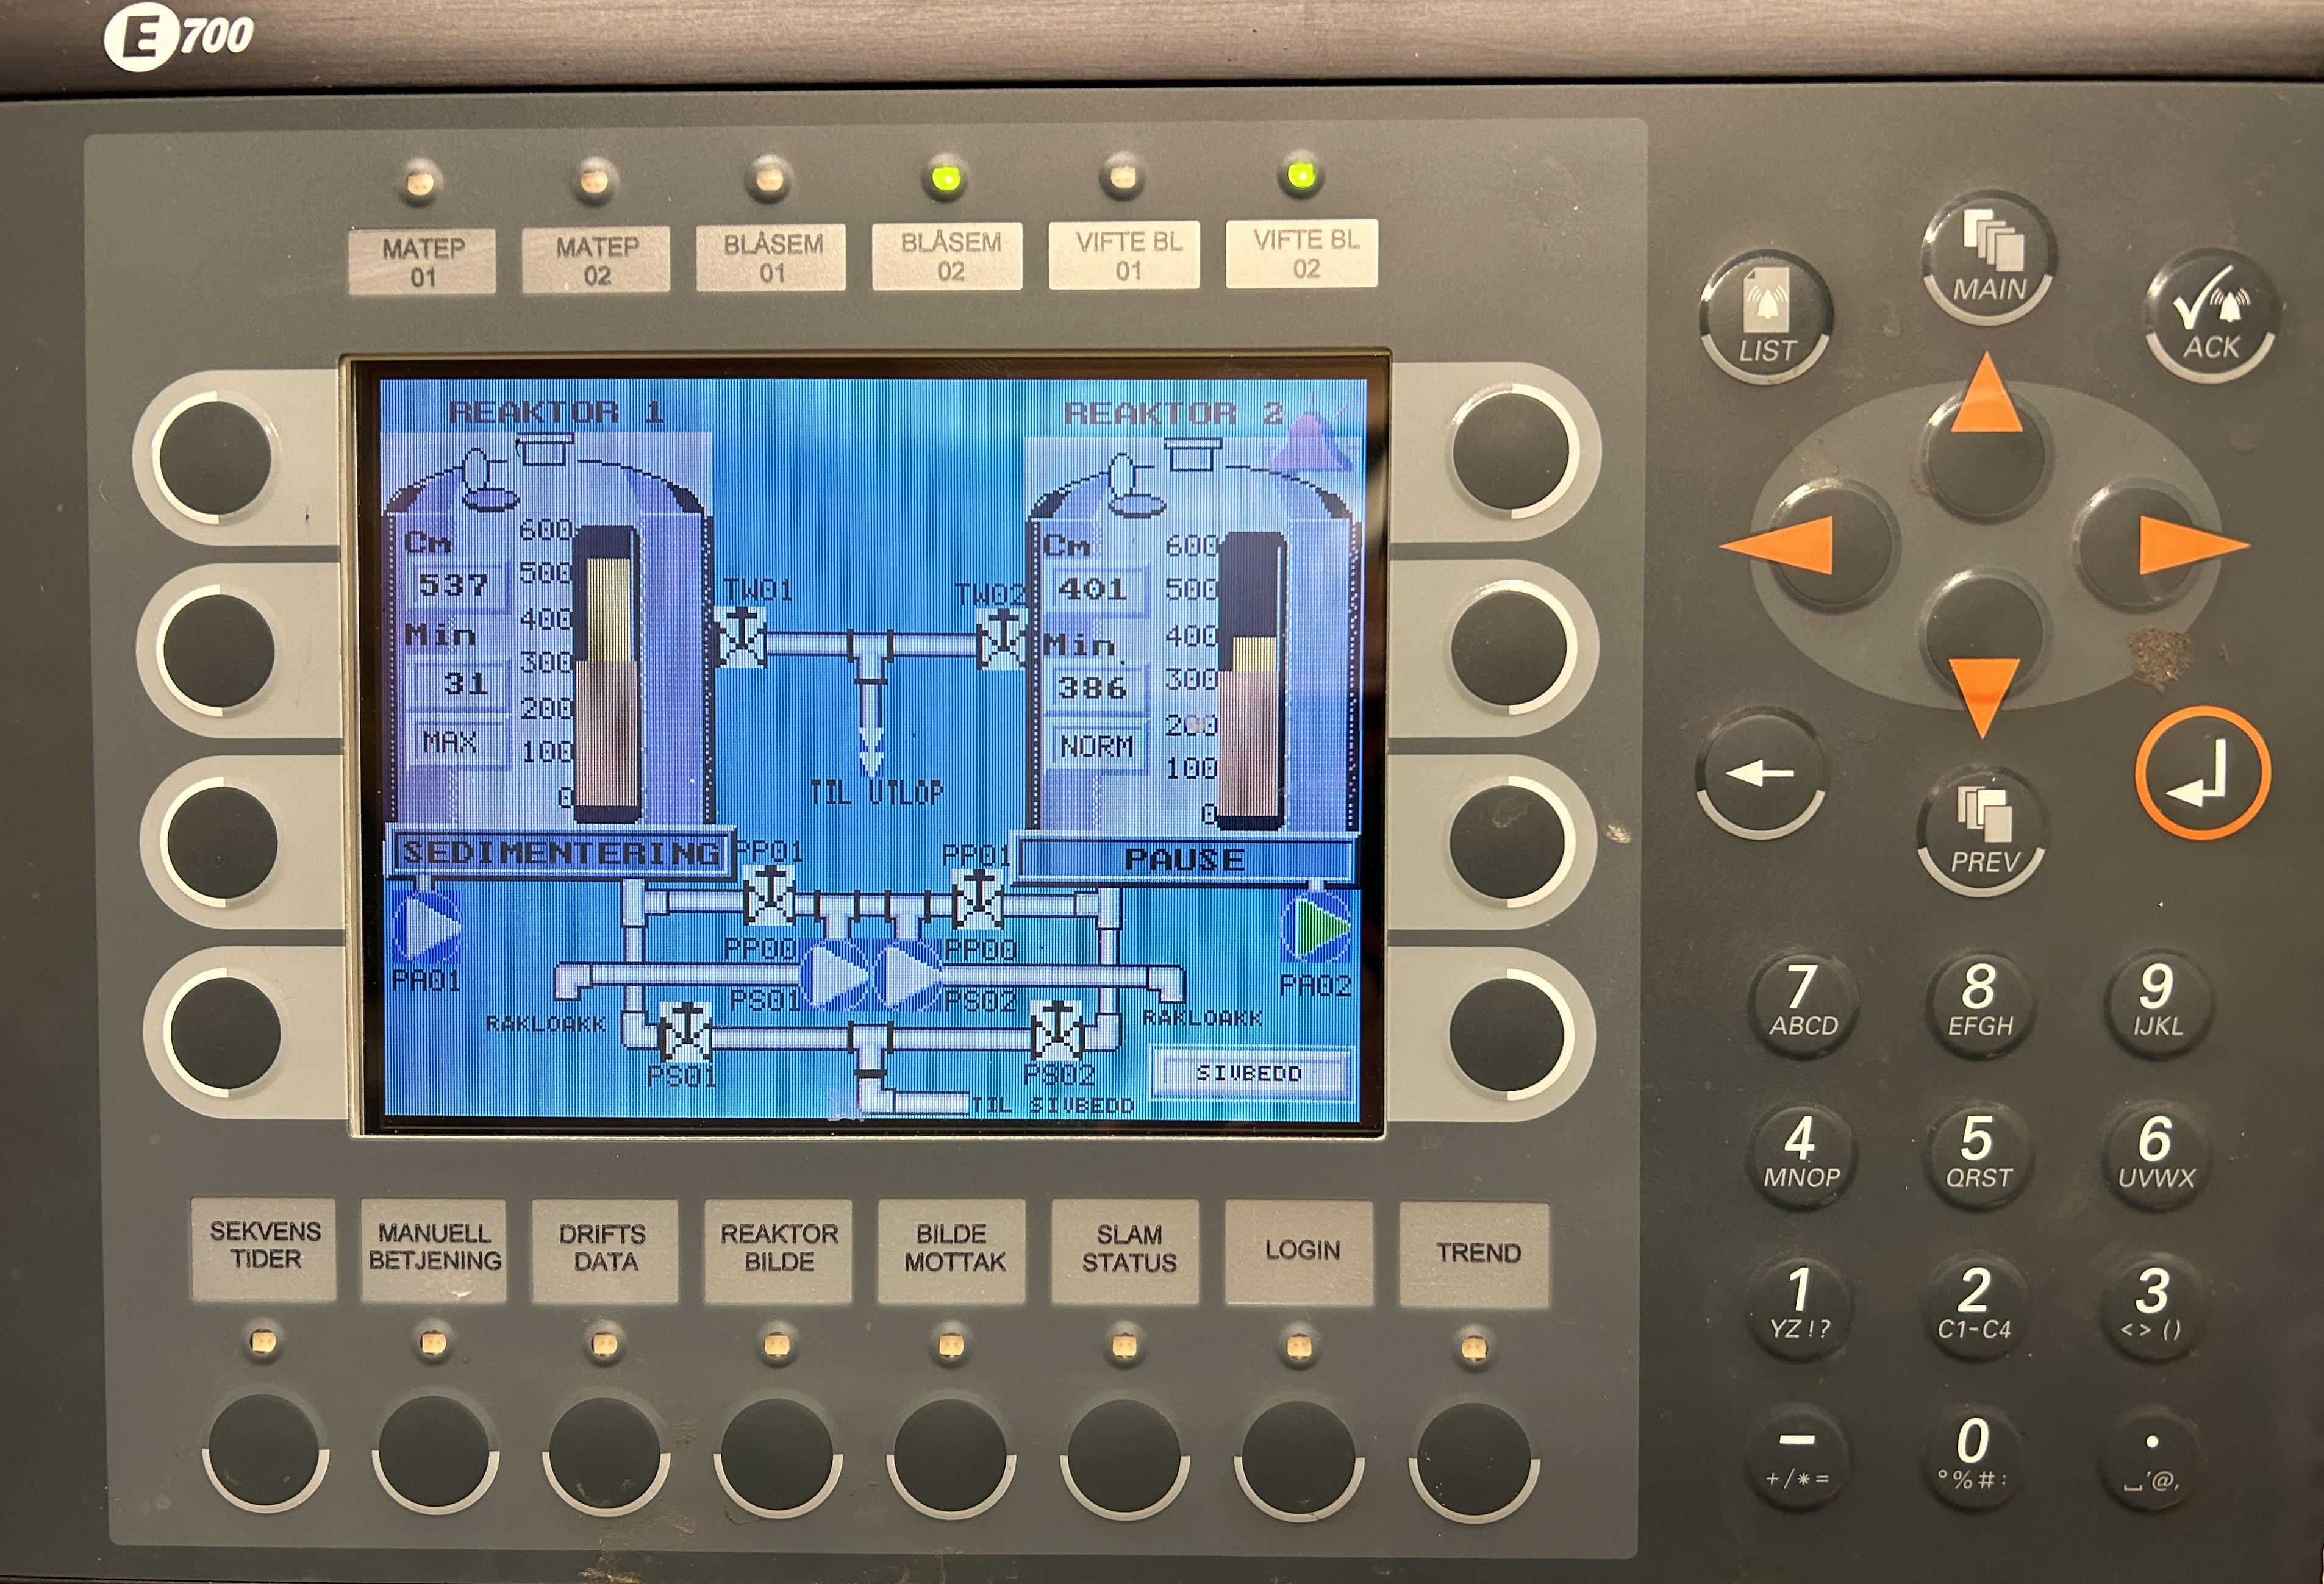
\includegraphics[width=1\textwidth]{Bilder/BeijerSkjerm.JPG}
        \caption{Beijer \gls{HMI}}\label{fig:BeijerSkjerm}
    \end{subfigure}
    \hfill
    \begin{subfigure}[b]{0.3\textwidth}
        \centering
        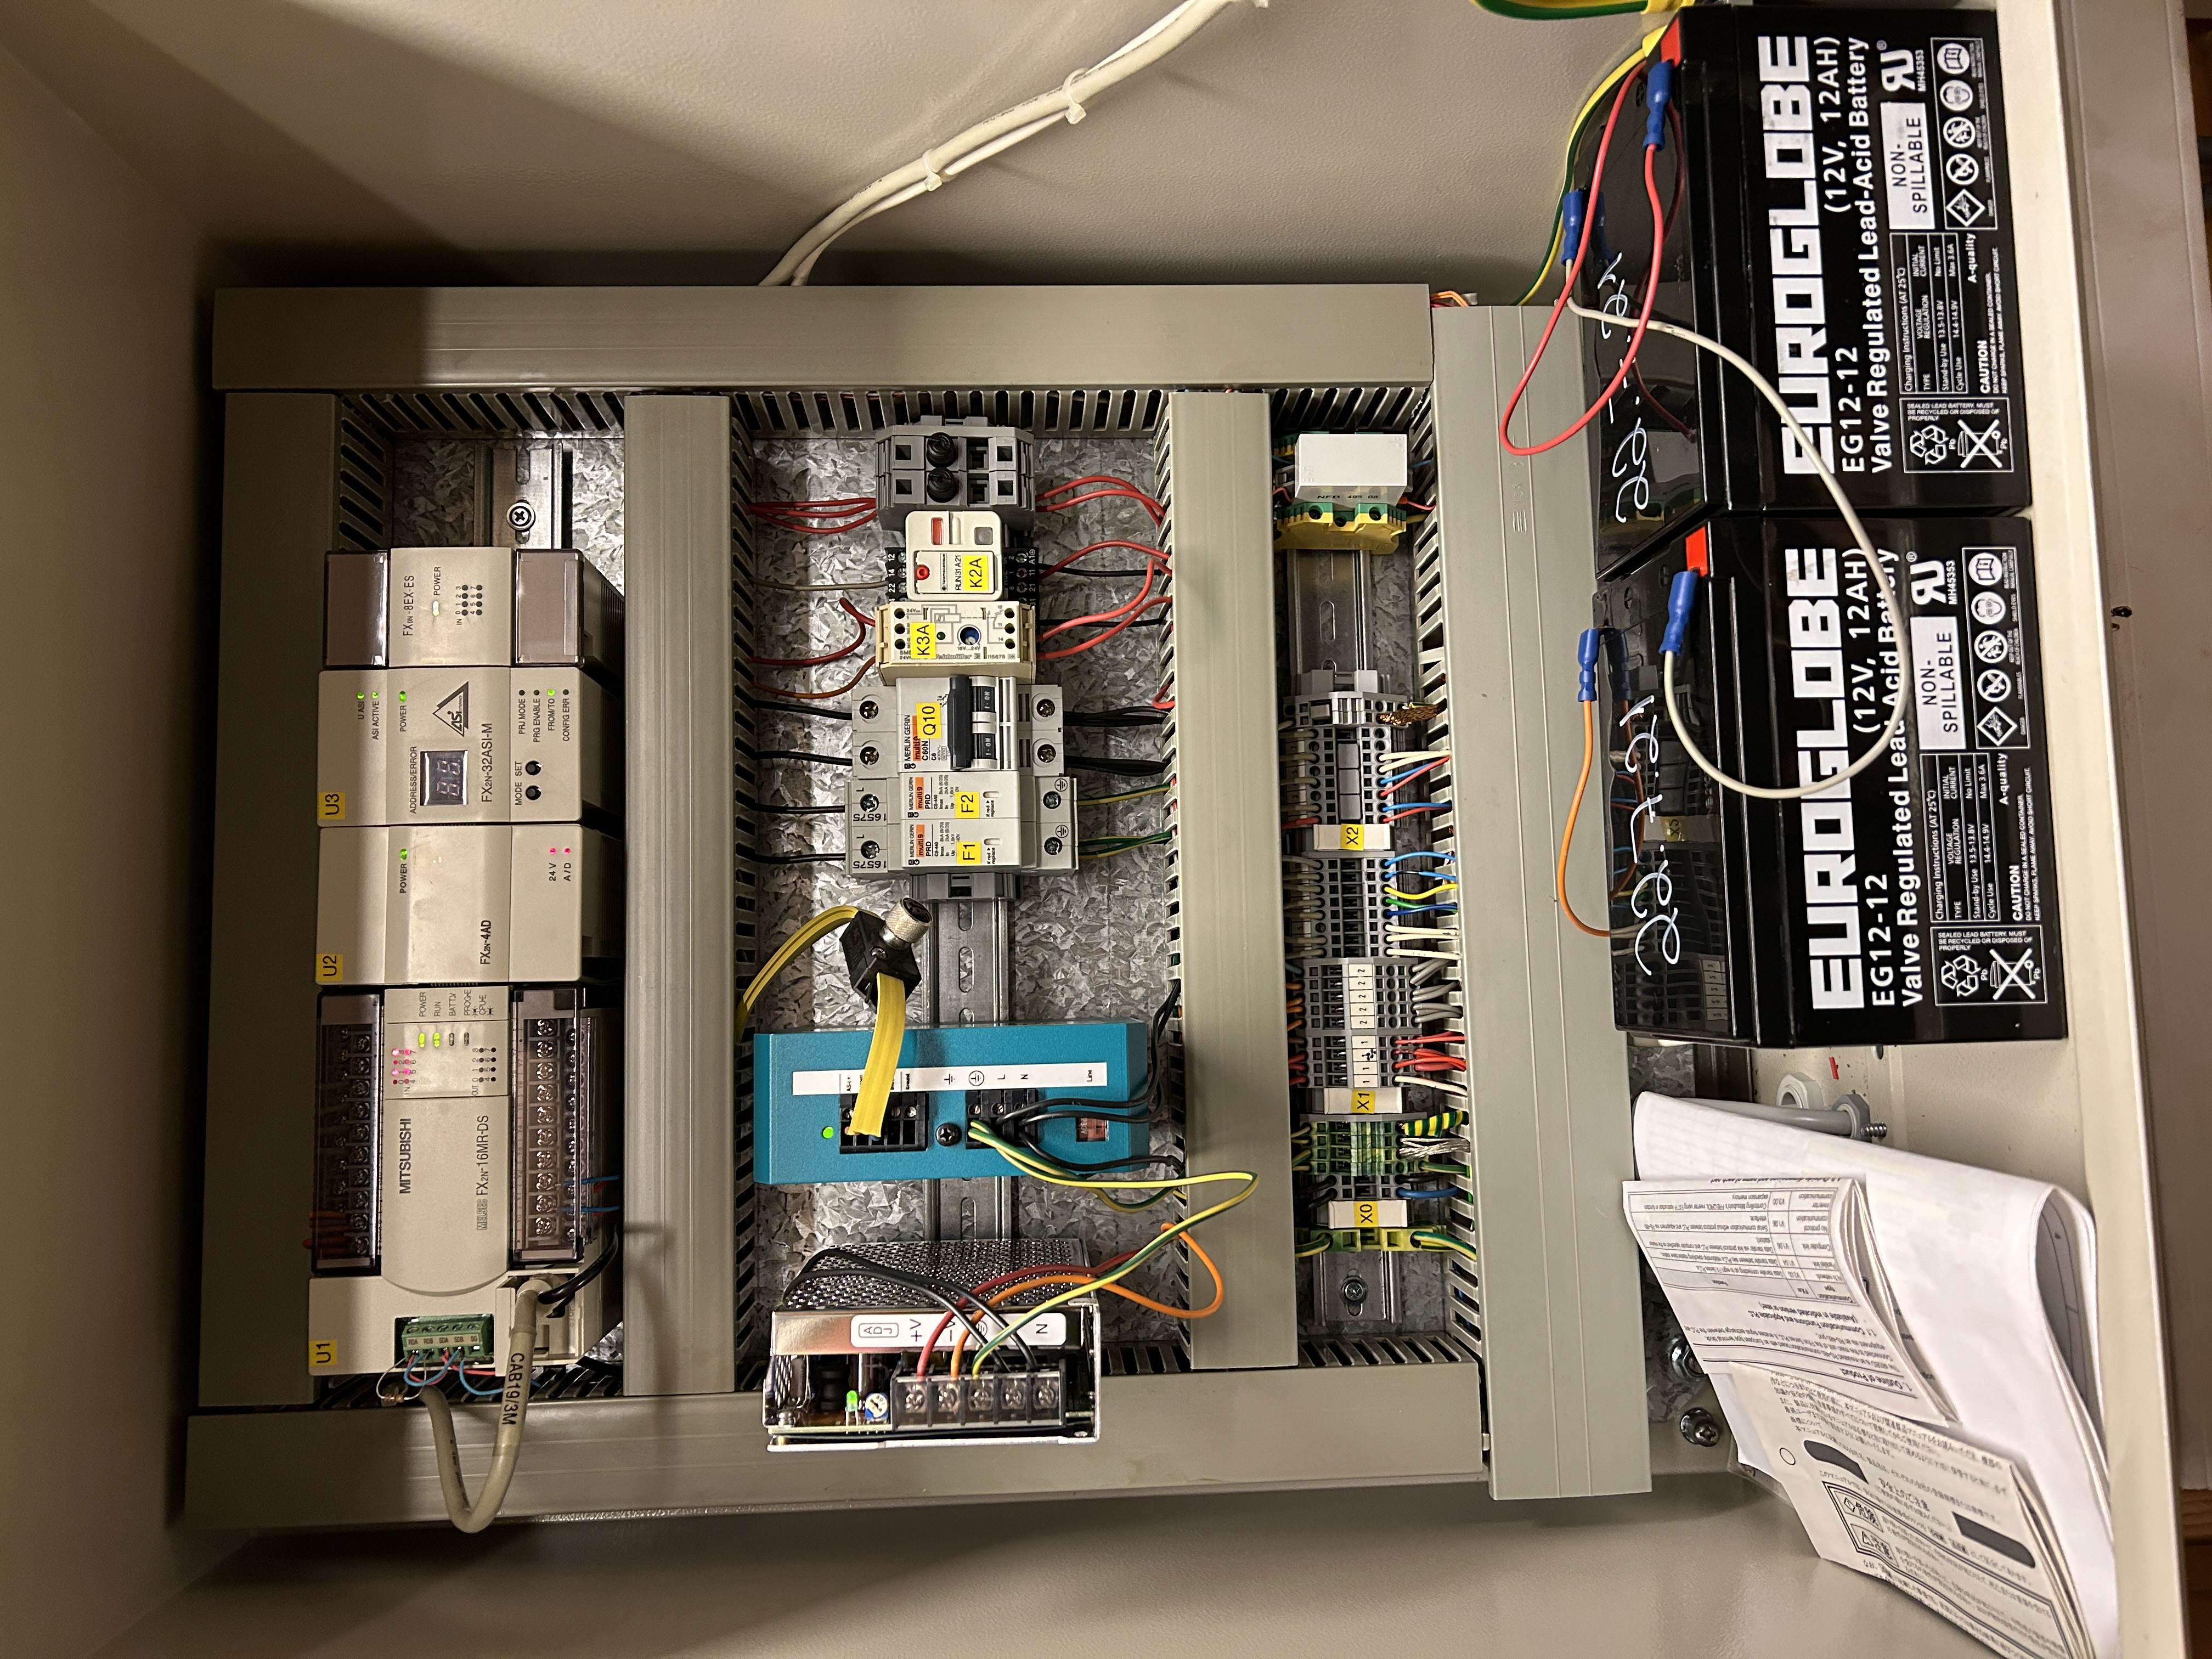
\includegraphics[angle=-90,width=1\textwidth]{Bilder/Styreskap.JPG}
        \caption{Styreskap}\label{fig:Styreskap}
    \end{subfigure}
    \caption{Styresystem}\label{fig:Styresystem}
\end{figure}

	\input{Tekst/Kapittel4 - Analyse av problemet/4.2 - Løysningsforslag.tex}
	\input{Tekst/Kapittel4 - Analyse av problemet/4.3 - Val og drøfting.tex}
	
	% Kapittel 5 Krav og mål
	\chapter{Krav og mål}
\thispagestyle{fancy}
\gls{Renasys} hadde som ynskje at vi etablerte kravspesifikasjonen til oppgåva 
i samråd med \gls{Sunnfjord Kommune}.\newline
Vi hadde eit møte med kommunen der dei kom med nokon konkrete ynskjer til oppgåva
og løysningsforslaget vi hadde presentert.

\begin{enumerate}
    \item Unngå høge lisenskostandar i planlegginga rundt ny PLS og val av programmeringsverktøy.
    \item Oprette ein funksjonsbeskrivelse som forklarer korleis anlegget virker.
    \item Undersøke og planlegge forbetringar av anlegget ved hjelp av ny sensorikk.
\end{enumerate}

%\begin{enumerate}
    %\item Overgang frå system med høge lisenskostandar og utskifting av PLS
    %\item Forbetring og utvikling av ny dokumentasjon, som inkludera ein ny funksjonsbeskrivelse 
    %\item Undersø
%\end{enumerate}

\section{Krav}
Vi tok utgangspunkt i ynskja frå \gls{Sunnfjord Kommune} for å forme kravspesifikasjon vår.
Deretter utarbeida vi ei liste med krav som naturleg delte seg i tre
hovuddelar: dokumentasjon, programmering og simulering med verifisering. 
Denne oppdelinga vart framlagt for oppdragsgivarane og godkjent. 

\begin{enumerate}
    \item Dokumentasjon:
    \begin{itemize}
        \item Dokumentere anlegget og opprette ein funksjonsbeskrivelse.
        \item Dokumentere det nye styresystemet.
    \end{itemize}
    \item Programmering, vi skal:
    \begin{itemize}
        \item Programmere etter den nyoppretta funksjonsbeskrivelsen.
        \item Anvende open kjeldekode og ikkje låse anlegget til ein spesefikk leverandør.
    \end{itemize}
    \item Simulering med verifisering
    \begin{itemize}
        \item Simulere og teste det nye programmet
    \end{itemize}
\end{enumerate}


%, fjernet "som vart gjort i samråd med rettleiar"

%\begin{enumerate}
    %\item Dokumentasjon med detaljert funksjonsbeskrivelse som inneheld:
        %\begin{itemize} 
        %\item Beskriving av anleggets verkemåte
        %\item \gls{blokkdiagram}
        %\item \gls{forrigling}, \gls{alarm}- og \gls{IO}-lister
        %\item Oversikt over objekta
        %\item \gls{PID}
        %\end{itemize}
    %\item Programmering, vi skal:
        %\begin{itemize}
        %\item Bruke den ny funksjonsbeskrivelsen som grunnlag for programmet.
        %\item Anvende open kjeldekode og ikkje låse oss til spesifikke leverandørar.
        %\end{itemize}
    %\item Simulering med verifisering
        %\begin{itemize}
        %\item Utvikle eit simuleringsverktøy for å teste og verifisere programmet
        %\end{itemize}
%\end{enumerate}

%\newpage

\section{Mål}
Utan om kravspesifikasjonane som var avklart med arbeidsgivar satt vi oss
også nokre personlege mål for oppgåva.

\begin{itemize}
    \item Breie vår kompetanse og bruke eit nytt programmeringsprogram.
    \item Programmere eigne funksjonsblokker som anvender relevante industri standarar.
    \item Levere eit program som er lett å annvende og enkelt å vedlikehalde.
    \item Implementere tilstandsmaskin som styringsform.
\end{itemize}

%\section{Ny funksjonalitet og sensorar}
%Følgande funksjonar og sensorar er ikkje nødvendig for programmets grunnleggande verkemåte, men 
%er ønska av \gls{Sunnfjord Kommune} om tiden strekker til.  
%\begin{itemize}
    %\item Temperatur, nivå og trykksensorar(reintvan inn).
    %\item Ventil tilbakemeldingar og oksygenmåling
    %\item Mengdemåling for overlaup og frekvensstyring av pumper
    %\item Integrasjon av \gls{MJK} prøvetakar og energimåling
%\end{itemize}



	% Kapittel 6 - Anleggets Verkemåte
	\chapter{Verkemåten til anlegget}\label{sec:6}
\thispagestyle{fancy}

For å sette oss inn i korleis Sande reinseanlegg fungerar var vi nøydd til å forstå
korleis eit generelt avlaupsreinseanlegg er oppbygd. Dette var det naturlege første
steget inn mot løysningsalterntivet vi valde. 



	\section{Generel verkemåte}

Eit avlaupsreinseanlegg er bygd opp av 3 hovuddelar: Primær, sekunder og tertiærreinsing,
samt ein del for behandling av slam.
Alle desse delane kan løysast på forskjellige måtar, men hovudoppgåvene er dei same
i alle reinseanlegg.

``Primærreinsing'' handlar om å skille organisk og uorganisk materiale.
I eit avlaupsreinseanlegg tilsvarer dette å skille avlaupsvatnet, 
som ein vil behandle frå, sand, Q-tips, våtserviettar
og anna uønska material som ein ikkje ynskjer vidare i prosessen.\newline
``Primærreinsing'' er eit viktig steg for å beveare pumper og anna prosessutstyr.

``Sekunderreising'' handlar om å fjerne mest mulig suspanderte stoffer og organisk materiale.
Det tilsvarer å skilje det meste av organisk materialet frå vatnet.
``Sekunderreising'' er i kvart anlegg avhengig av kva `reinseprinsipp' som er brukt. Dette tilsvarer
kva teknolgisk metode som nyttast for å utføre dette steget.
``Sekunderreising'' refererast oftast til biologiskreinsing.

``Tertiærreising'' handlar om å fjerne resterande forureiningar i vatnet.
Dette steget varierer veldig frå anlegg til anlegg og eg er
avhengig av kva krav reiseanlegget har som krav på sitt utslippsvatn.

Slamebehandling handler om å fjerne og behandle det oppbygde organiske materialet (Slam)
som skillast ut i sekundær og tertiærreinsing 

\begin{figure}[htbp]
    \centering
    \includegraphics[width=1\textwidth]{Figurar/Generellverkemåte.png}
    \caption{Generell verkemåte for eit avlaupsreinseanlegg}\label{fig:GenerellVerkemåte}
\end{figure}

Når vi hadde satt oss inn i den generelle verkemåten til eit avlaupsreinseanlegg
valgte vi å fokusere mot Sande.
Dette valgte vi å gjere i tre hovuddelar. Kva reinseprisipp er brukt, korleis Sande reinseanlegg
fungerar i praksis og om anlegget har nokre særeigna preg.

	\newpage
\section{Teknisk verkemåte}
\thispagestyle{fancy}
Sande reinseanlegg er konstruert og basert på \gls{SBR}-teknologi.

\gls{SBR} står for ``Sequence \Gls{Batch} Reactor'', på norsk ``sekvensiell \gls{Batch}reaktor''.\newline
\gls{SBR} er en reinsemetode der alle prosessar føregår i same reaktortank. 
Reaktor nyttar biologisk reinsing, ved hjelp av aktivert slam som inneheld mikroorganismar, for å koagulere 
og å fjerne løyste og ikkje sedimenterbare partiklar samt stabilisere organisk materiale. 
Avlaupsvatn tilførast reaktor i ``\gls{Batch}er'' for å bli behandla. 
Kvar avlaups-\gls{Batch} går gjennom ein reaktorsyklus som består av følgjande fem delsekvensar \citep{Statsforvalter}.
\newline

\begin{figure}[htbp]
    \centering
    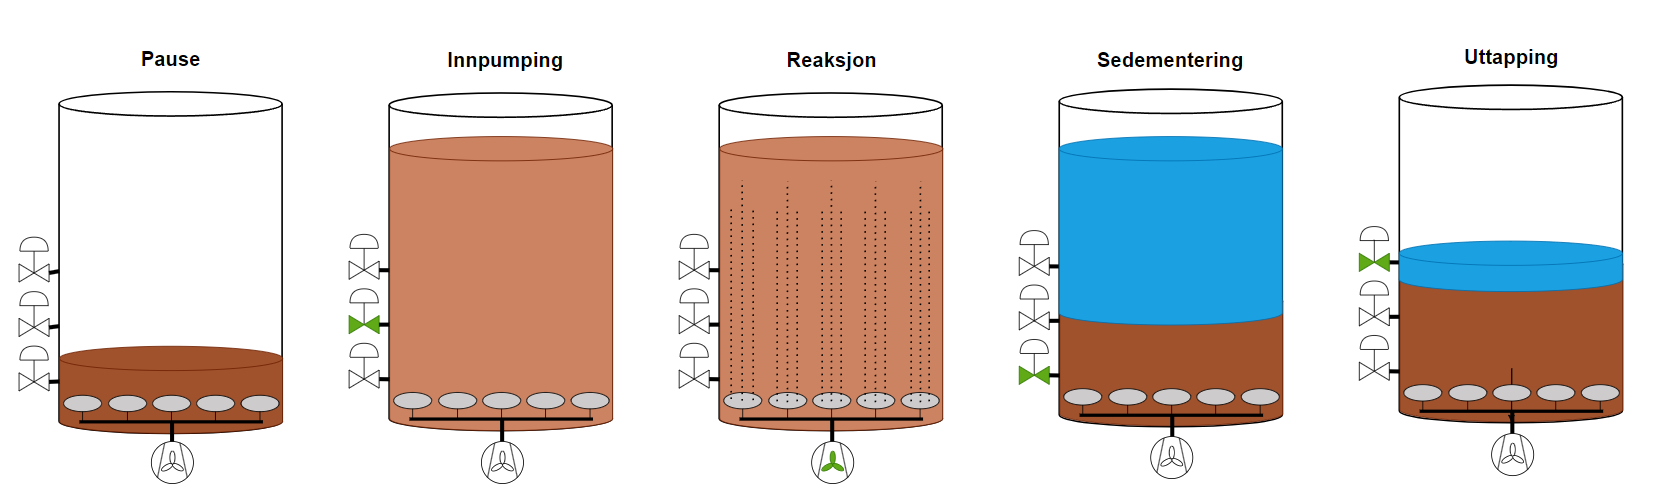
\includegraphics[width=1\textwidth]{Figurar/SBR-V2.png}
    \caption{\gls{SBR}-prosessen}\label{fig:SBR-Prosessen}
\end{figure}


\begin{enumerate}
    \item \textbf{\makebox[3cm][l]{Pause}:} Reaktor er klar og ventar.
    \item \textbf{\makebox[3cm][l]{Innpumping}:} Reaktor mottar avlaupsvatn, normalt frå ein utjamningstank.
    \item \textbf{\makebox[3cm][l]{Reaksjon}:} Reaktor luftast periodisk for å tilføre oksygen til mikroorganismane.
    \item \textbf{\makebox[3cm][l]{Sedimentering}:} Reaktor sedimenterer ved hjelp av gravitasjon. Overskuddslam fjernast.
    \item \textbf{\makebox[3cm][l]{Uttapping}:} Reaktor drenerar reinsavatn mot resipient.
\end{enumerate}

Meir detaljert informasjon om \gls{SBR} og anleggets teknolgiske prinsipp er tilgjengeleg, via vedlegg, i anleggets nye
funksjonsbeskrivelse. (Vedlegg A)


	\newpage
\section{Praktisk Verkemåte}
\thispagestyle{fancy}

Sande reinseanlegg består av 'primærreinsing' via grovrist, ein mottakstank 
som samlar varierande tilstrøymingar for å gi resten av anlegget homogene forhold og
'sekundær' og 'tærtierreinsing' ved to reaktorar som anvender \gls{SBR}-teknologi.

Avlaupsvatnet vil opphalde seg i eller på veg mot ein av desse fire hovuddelane medan det er i anlegget.
Ferdig behandle avlaupsvatn blir drenert ut til elva Gaula. 

\begin{figure}[htbp]
    \centering
    \includegraphics[width=1\textwidth]{Figurar/Sande verkemåte.png}
    \caption{RA200 flytskjema}\label{fig:HMI}
\end{figure}

\subsection{Grovrist}
Innløpet på anlegget renn først igjennom grovrista. Grovrista på reinseanlegget
er ein (Huber rotomat R09). Grovrista fungerer som ein liten tank og ein intern nivågivar startar
skruen ved innkommande avlaupsvatn. Skruen tek med uorganisk materiale og fjernar det til eigen avfallshandtering.
Dersom grovrist feiler vil vatnet renne vidare til mottakstanken via eit overløpsrøyr.

\begin{figure}[htbp]
    \centering
    \begin{subfigure}[b]{0.3\textwidth}
        \centering
        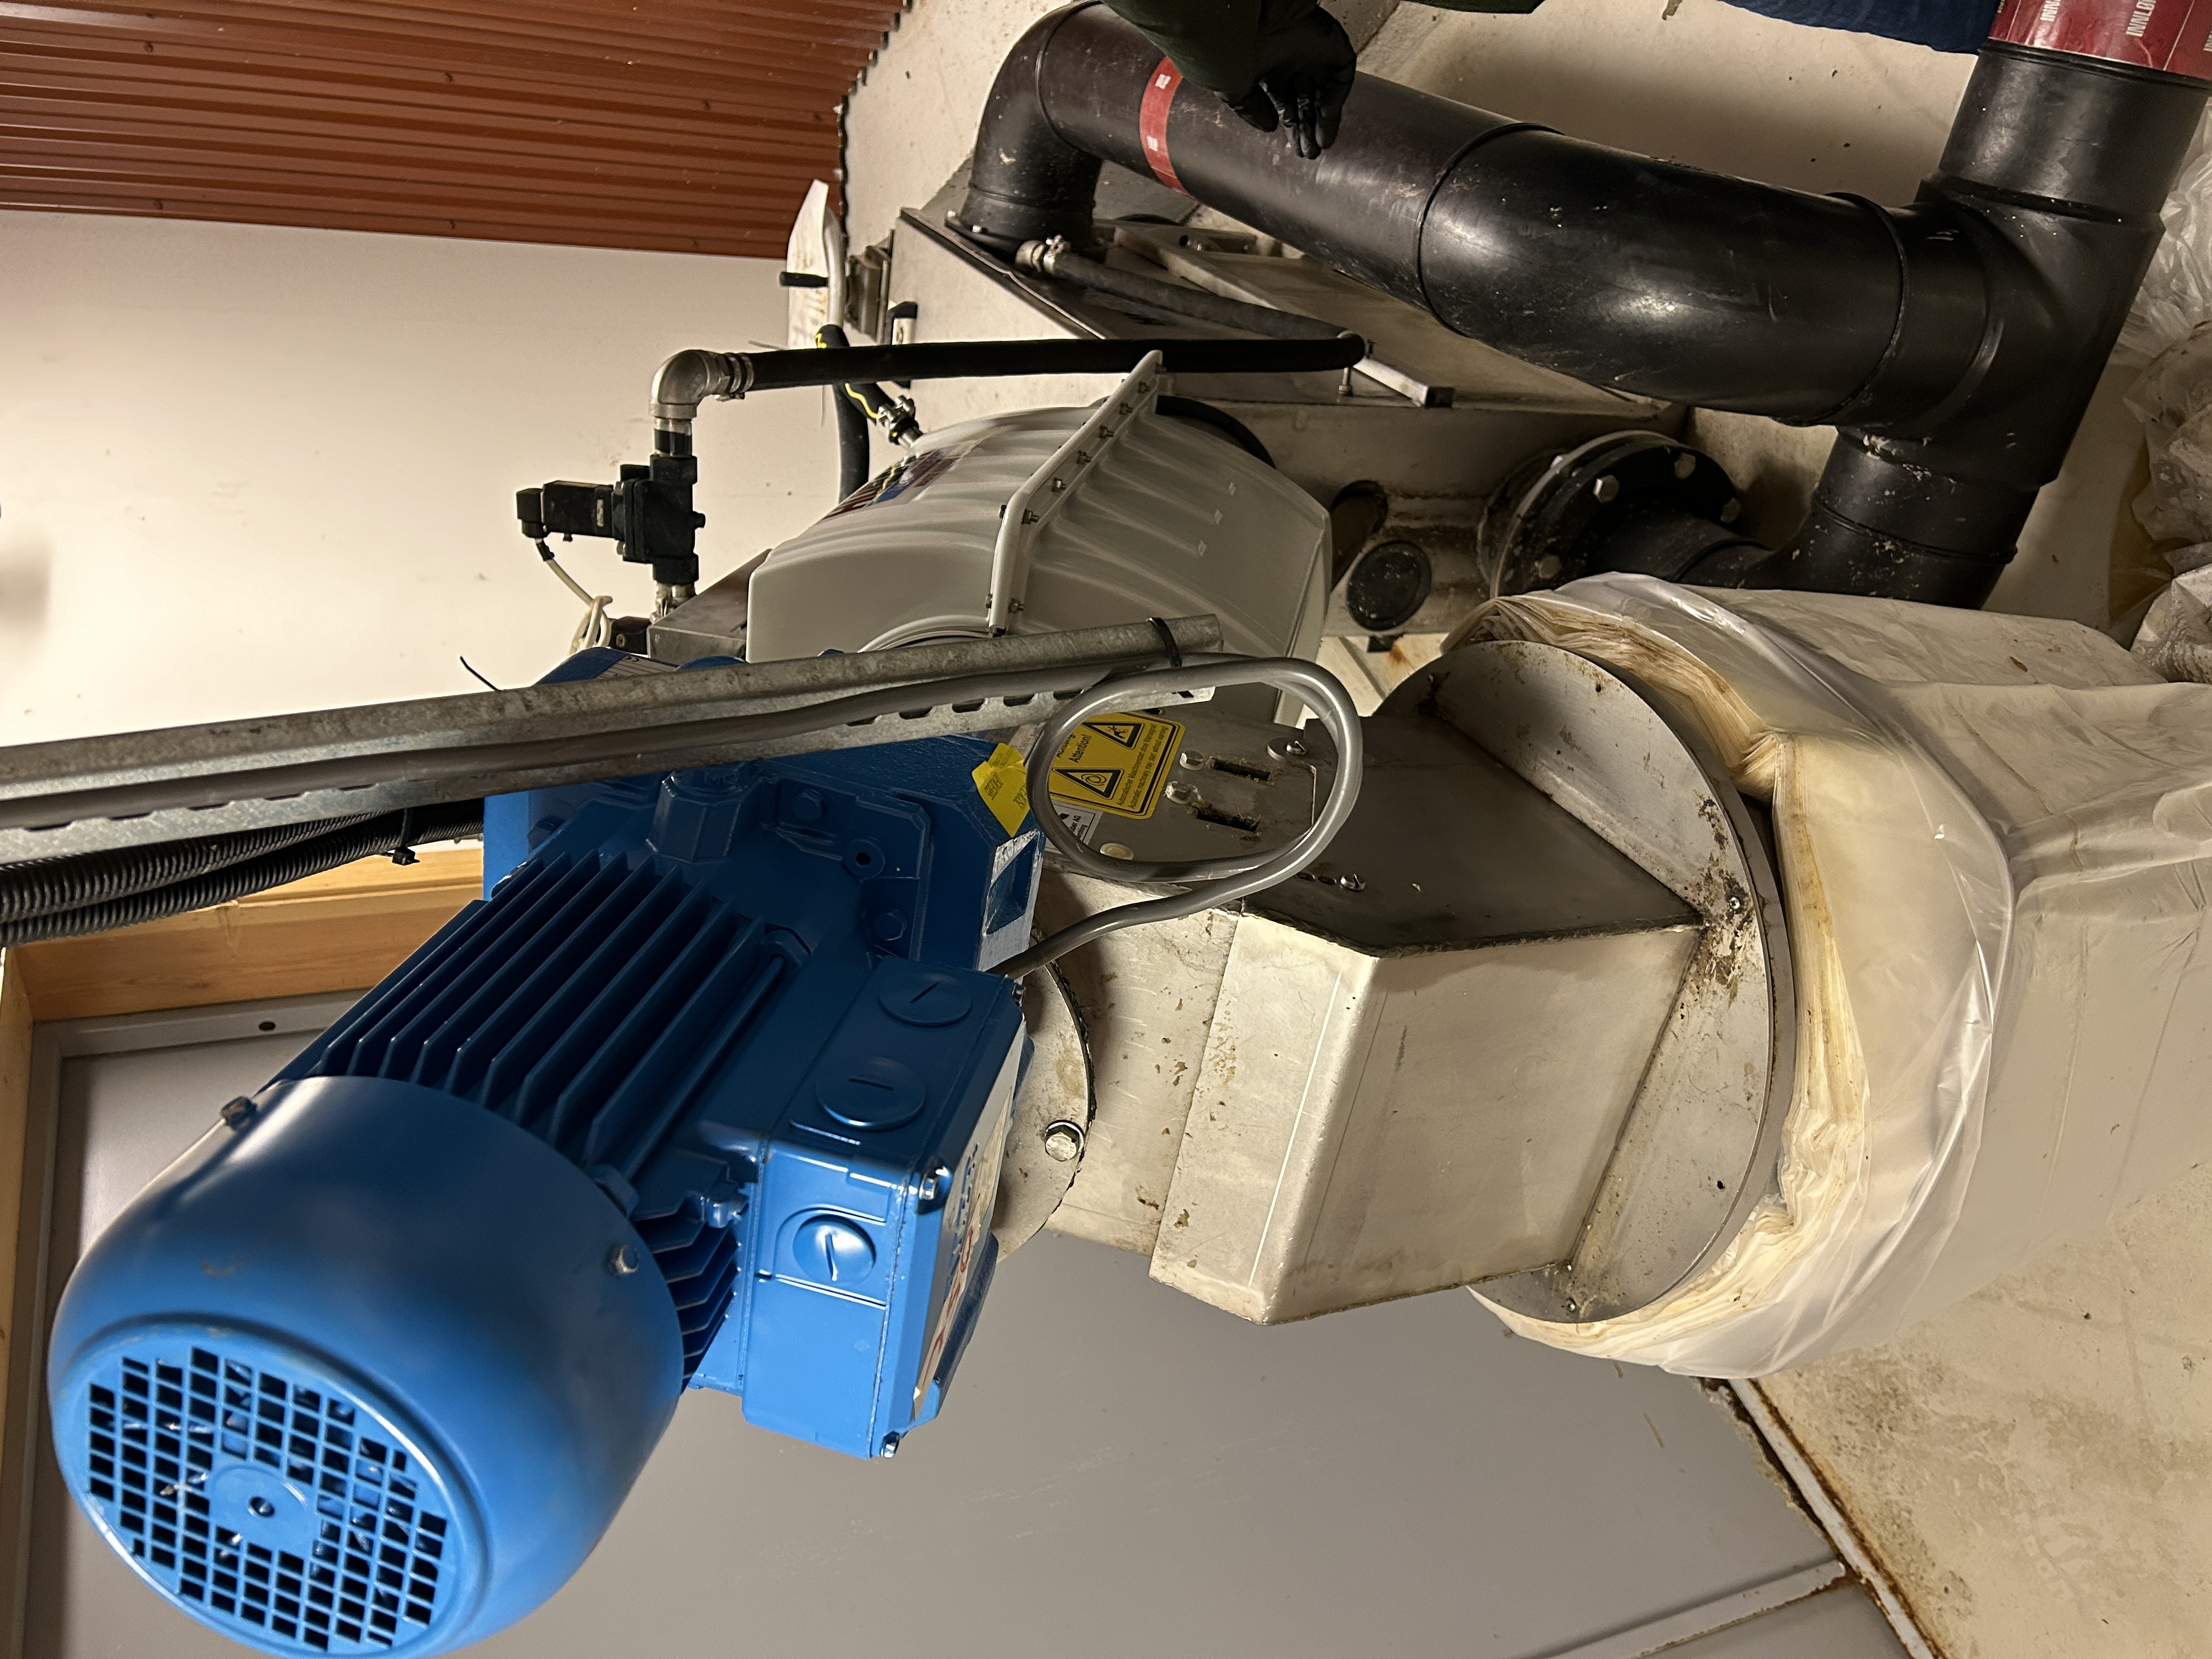
\includegraphics[angle=-90,width=1\textwidth]{Bilder/Huber.JPG}
        \caption{Motor og avfallshandtering}\label{fig:subfig1}
    \end{subfigure}
    \hfill
    \begin{subfigure}[b]{0.3\textwidth}
        \centering
        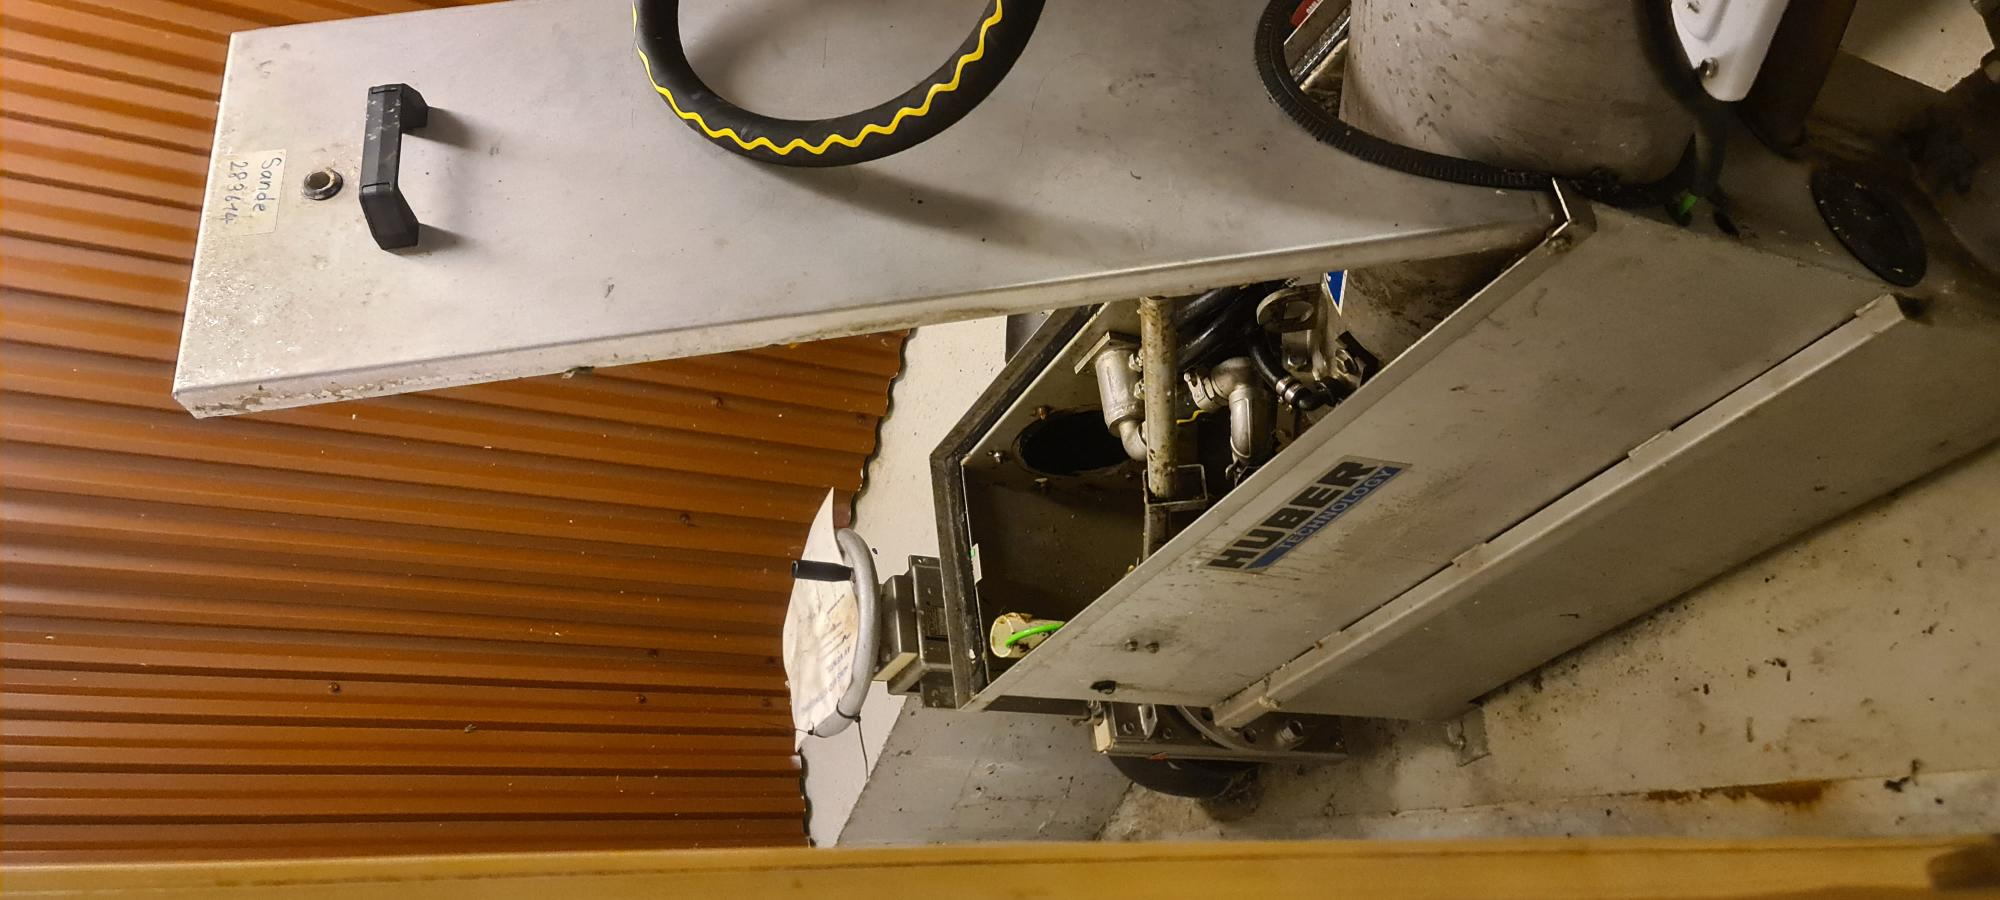
\includegraphics[angle=-90,width=0.6\textwidth]{Bilder/Huber2.JPG}
        \caption{Godts og skrue}\label{fig:subfig2}
    \end{subfigure}
    \caption{Bilete Huber grovrist}\label{fig:Illustrasjon-Diffuser}
\end{figure}

\newpage
\subsection{Mottakstank}
Frå grovrista renner vatnet med sjølvfall mot mottakstanken som ligger som lavaste punkt på anlegget.
Mottakstanken er 120 $m^3$ og er ein felles lagringsplass for vatnet før det går vidare mot reaktorane.
Mottakstanken har fire sensorar som heng ifrå taket.

\begin{itemize}
    \item Trykkgivar for nivå (PP00-LT01)
    \item Trykkgivar for overløp (PP00-LT02)
    \item Flottør-vippe lav (PP00-LS02)
    \item Flottør-vippe høg (PP00-LS01)  
\end{itemize}

Nivået i mottakstanken blir primært målt med trykkgivar LT01. For at vatnet skal pumpast vidare mot ein
reaktor i riktig sekvens må trykkgivar indikere at nivået er høgt nok. LS02 fungerar som backup.
I toppen av mottakstanken er det ei overløpskasse som drenerer mot resepient, her vil det
ved normale omstendigheter ikkje renne anna ein reinsavatn. Trykkgivar for overløp måler
dersom ureinsavatn renner i resepientrøyret.

%% Må endre på tegning fordi det eine navnet er feil. Ikkje reject frå sivbed.

\begin{figure}[htbp]
    \centering
    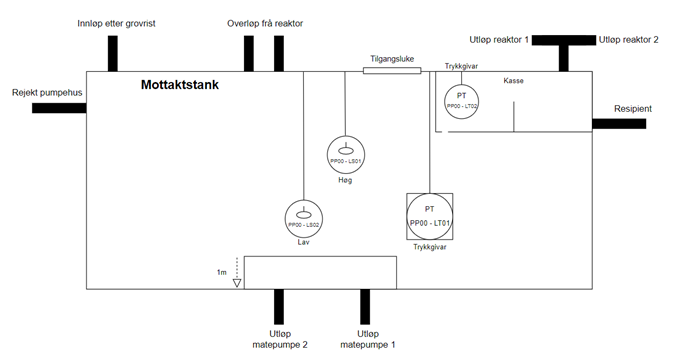
\includegraphics[width=1\textwidth]{Figurar/Mottakstank.png}
    \caption{P\&ID ottakstank}\label{fig:HMI}
\end{figure}

\begin{figure}[htbp]
    \centering
    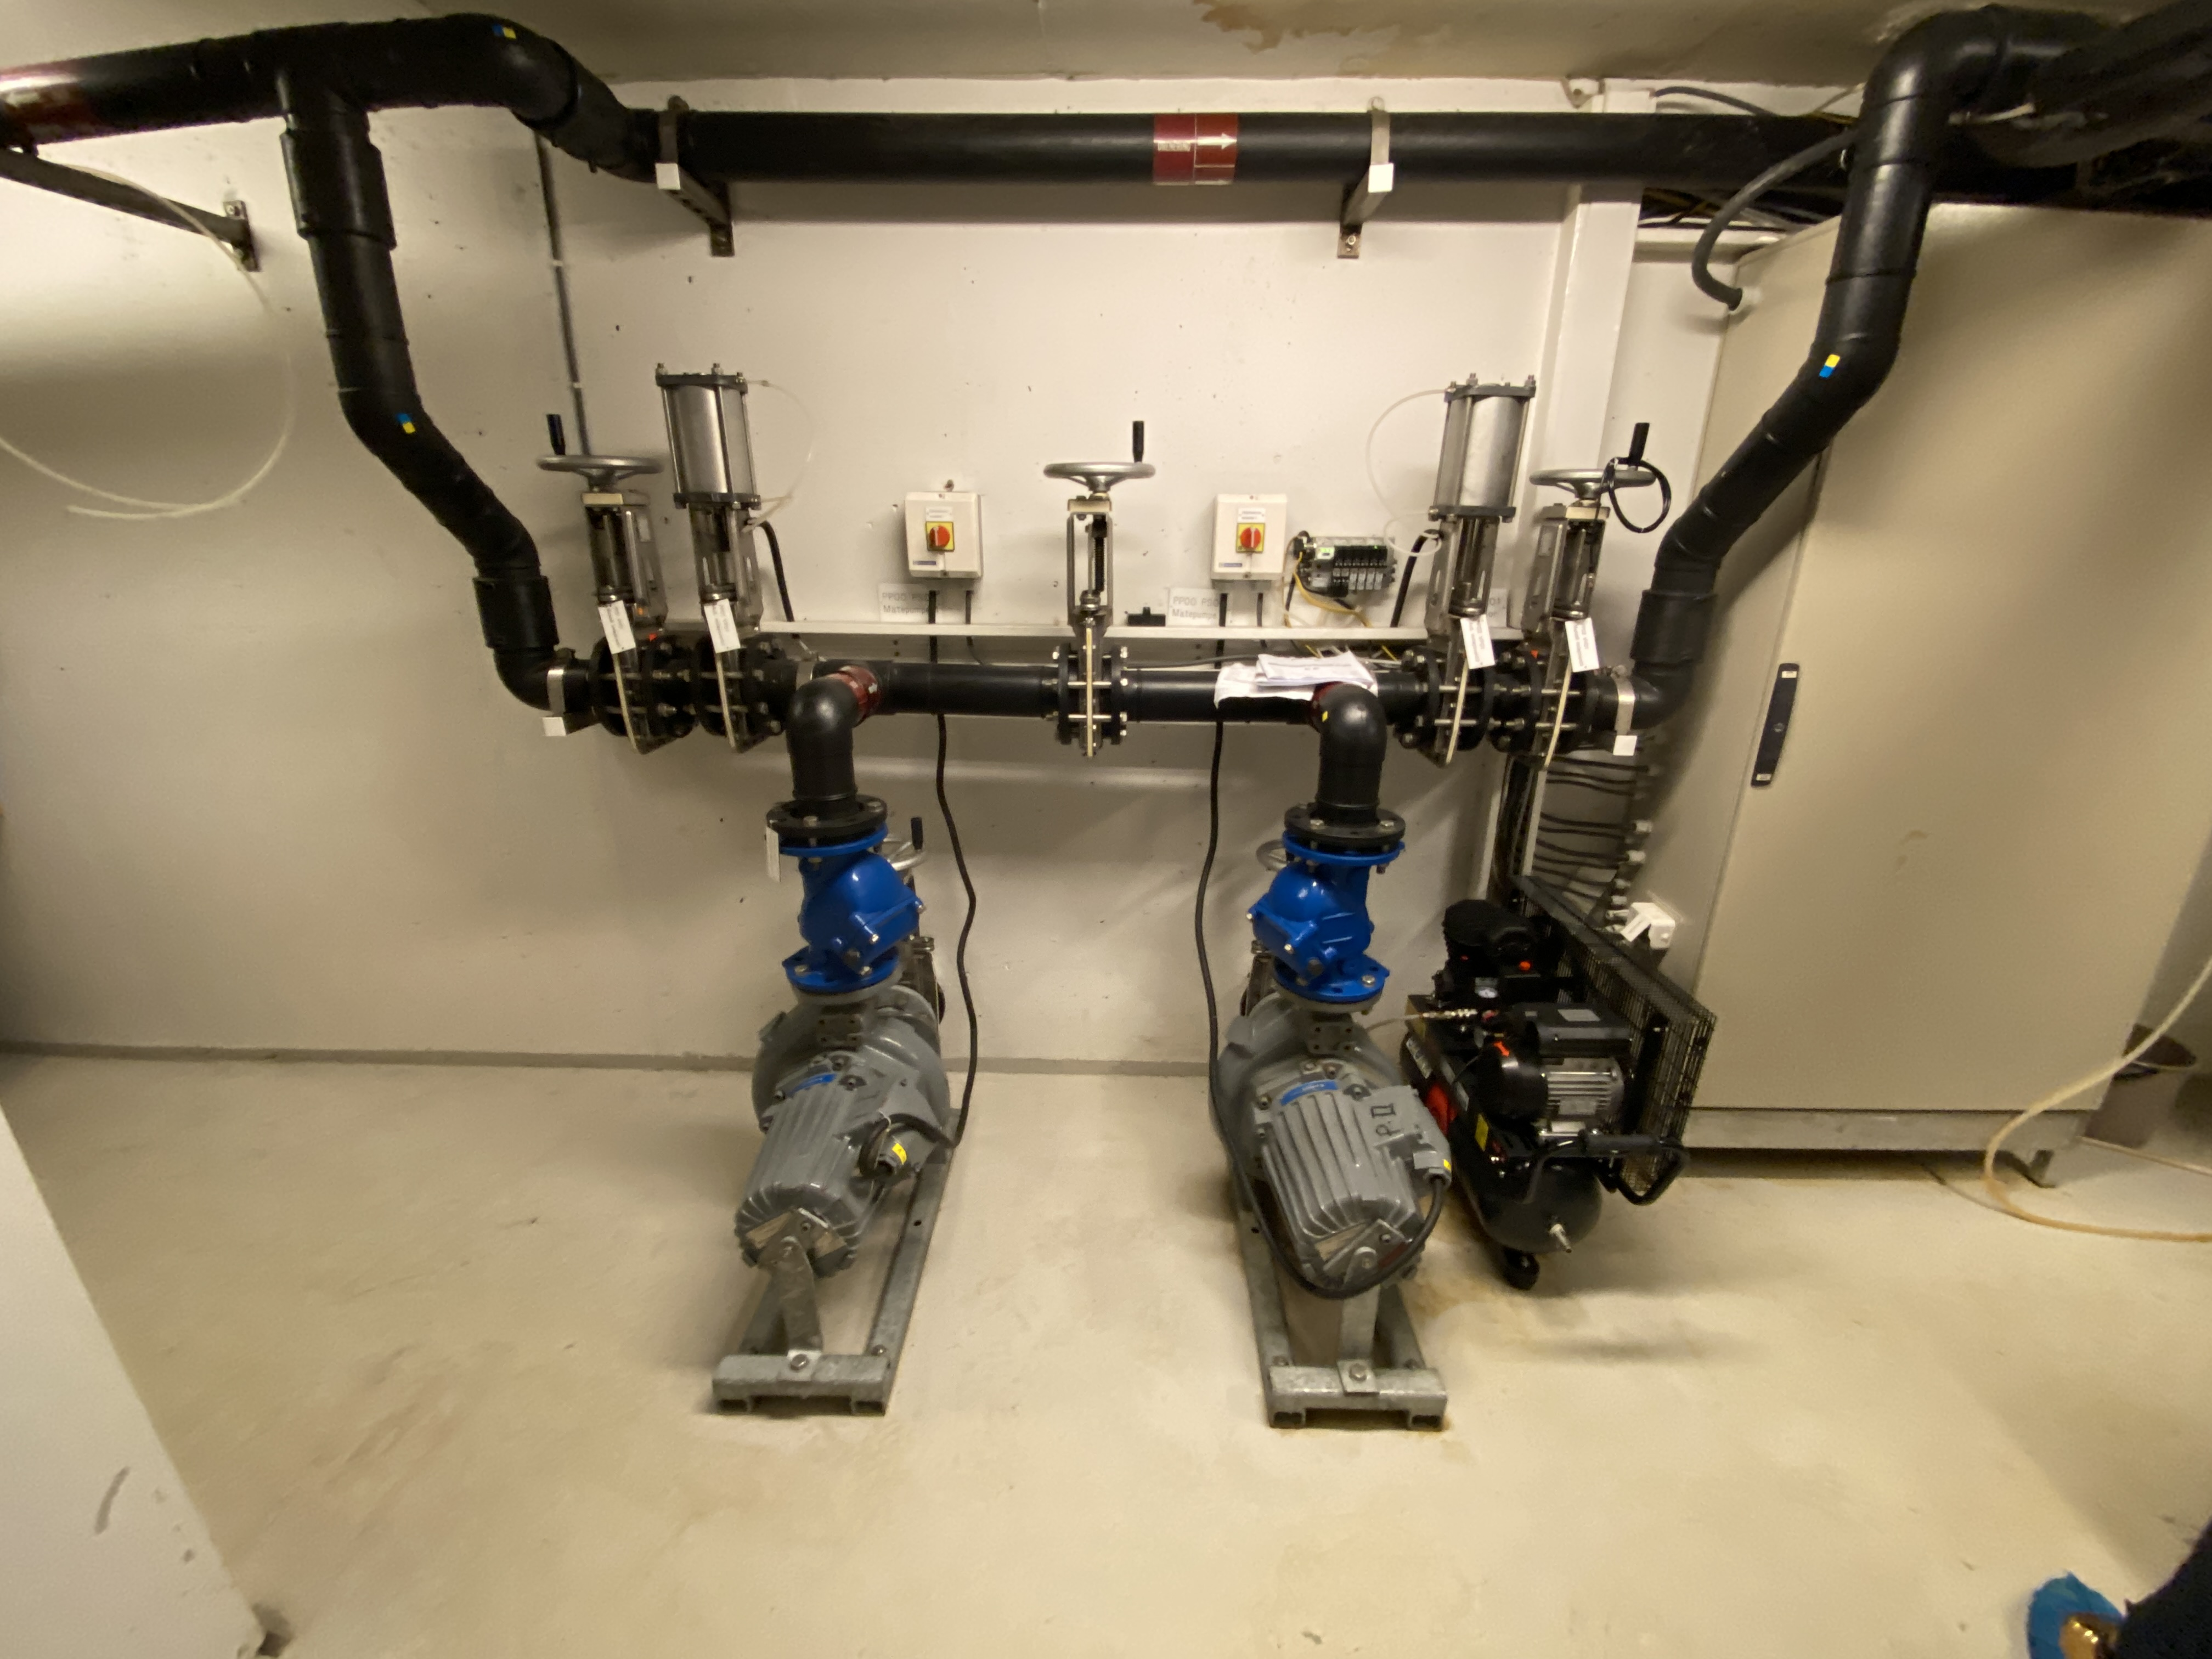
\includegraphics[width=1\textwidth]{Bilder/Bilde pumper.jpg}
    \caption{Matepumper}\label{fig:HMI}
\end{figure}

\newpage
\subsection{Reaktor}

Frå mottakstanken blir vatnet pumpa opp mot ein reaktor dersom den er i riktig sekvens.
Vatnet blir pumpa opp ved hjelp av to matepumper som rullerer, og kvar pumpe kan
levere til kvar reaktor. 
Reaktorane står på bakkenivå og strekker seg opp mot taket på bygget.
Reaktorane er utstyrt med nivåmåling via trykk. Trykksensoren står ca to meter over bunn av reaktor.

I reaksjonssekvensen blir reaktorane periodisk lufta. Dette er for å lage aerobe og anaerobe fasar
for mikroorganismane i reaktoraen som vidare gir betre reinsing.
For å for å best spreie oksygenet i den aerobe fasen
er det satt inn eit diffuser-oppsett i botn.
Diffurserane er laga av ein membran med små hull som dannar bobler når lufta kjem i 
kontakt med avlaupsvatnet.
Lufting av reaktoren gir også effektiv omrøring utan behov for ektra mekanisk inngrep.

\begin{figure}[htbp]
    \centering
    \begin{subfigure}[b]{0.3\textwidth}
        \centering
        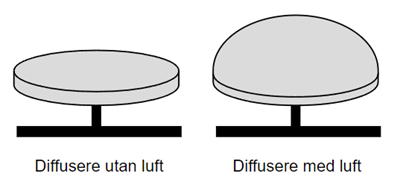
\includegraphics[width=1\textwidth]{Figurar/DiffusereMedOgUtanLuft.png}
        \caption{Illustrasjon diffuser}\label{fig:subfig1}
    \end{subfigure}
    \hfill
    \begin{subfigure}[b]{0.3\textwidth}
        \centering
        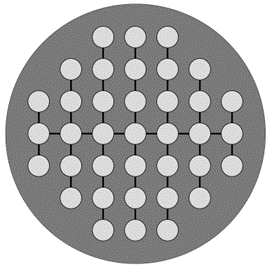
\includegraphics[width=1\textwidth]{Figurar/DiffuserFraTopp.png}
        \caption{Illustrasjon diffusere}\label{fig:subfig2}
    \end{subfigure}
    \caption{Illustrasjon oppsett av diffuser}\label{fig:Illustrasjon-Diffuser}
\end{figure}

På reiseanlegget er det ekstra krav for fjerning av fosfor. På grunn av desse ekstra krava
er det satt in eit tertiærreinse steg ved hjelp av simultanfelling.
Simultanfelling er ein fellesbetegnelse på kombinert biologisk og kjemisk reinsing.

I slutten på reaksjonsfasen tilsettest polyaluminium klorid, og kjemikaliet binder seg til
løyst fosfor og danner sedimenterbare partiklar. Desse sedimenterbare partiklane synker 
så i sedimenteringsfasen og utslippskravet på fosfor opprettholdast.

\begin{figure}[htbp]
    \centering
    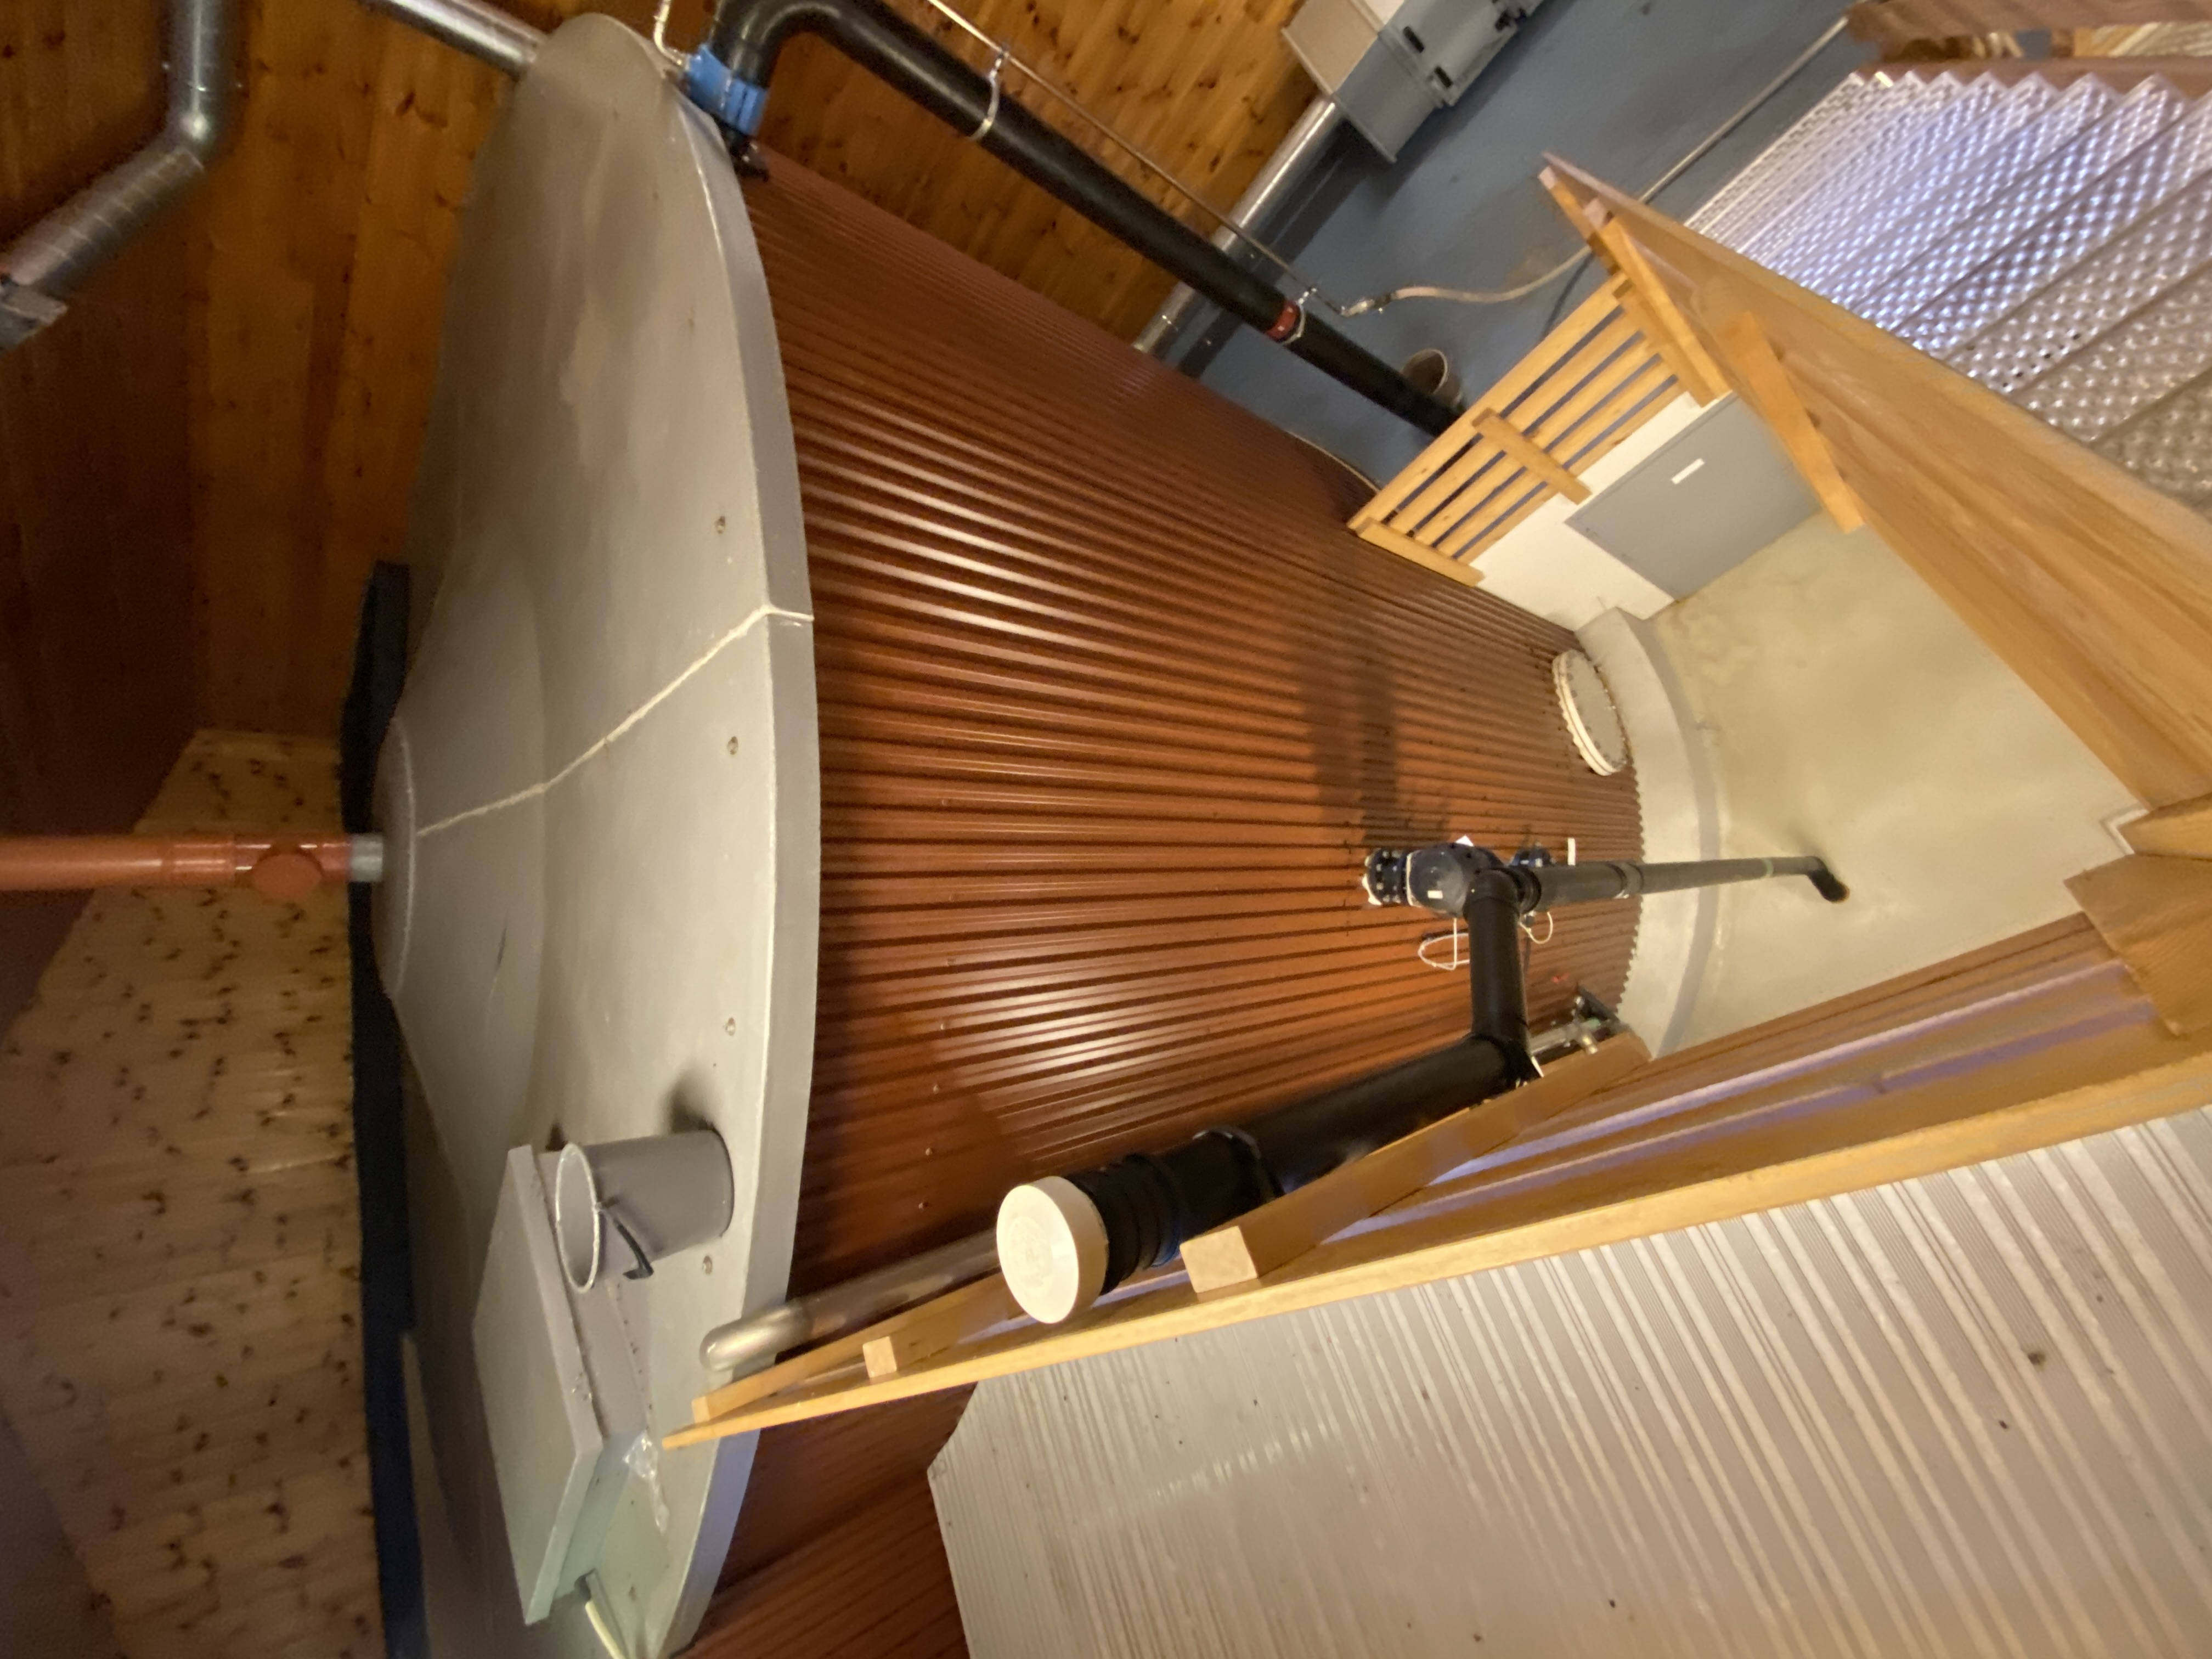
\includegraphics[angle=-90, width=1\textwidth]{Bilder/BildeReaktor.jpg}
    \caption{Reaktor}\label{fig:reaktorsoner}
\end{figure}

\newpage

Reaktorane er delt opp i tre forskjellige soner. Desse sonene er med på å skille
dei forskjellige medium når reaktoren er ferdig med ein syklus.
Alle SBR-reaktorar har lagra aktivert slam i botn. Det er her alle mikroorganismane akkumulerast
og gir grunnlag for god biologisk reinsing. Denne sona blir kalla slamsona.\newline
Alt over uttaksventilen er definert som bruksvolumet til reaktoren og det
er dette volumet som blir fylt og behandla kvar innpumpingsekvens.

Mellom dei to sonene eksisterer der ei sikkerheitssone.
Denne sona er til for å ta hand om varierande sedimenteringseigenskapar
og overskuddslam. \newline

\begin{figure}[htbp]
    \centering
    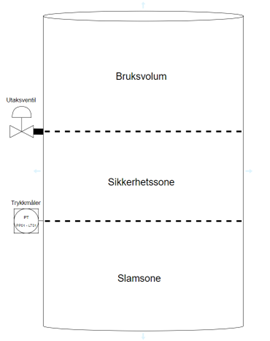
\includegraphics[width=0.5\textwidth]{Figurar/Reaktorsoner.png}
    \caption{Illustrasjon reaktorsoner}\label{fig:reaktorsoner}
\end{figure}

\subsection{P\&ID}

Det å setje seg inn i anleggets verkemåte skulle vise seg å være noko meir problematisk ein vi hadde forventa.
Hovudgrunnen til dette var at det ikkje fantest noko røyrgateskjema eller teknisk planteikning.
Vi ansåg det som naudvendig å etablere eit P\&ID diagram for å betre dokumentere og vise samanhengen til anlegget.

\begin{figure}[htbp]
    \centering
    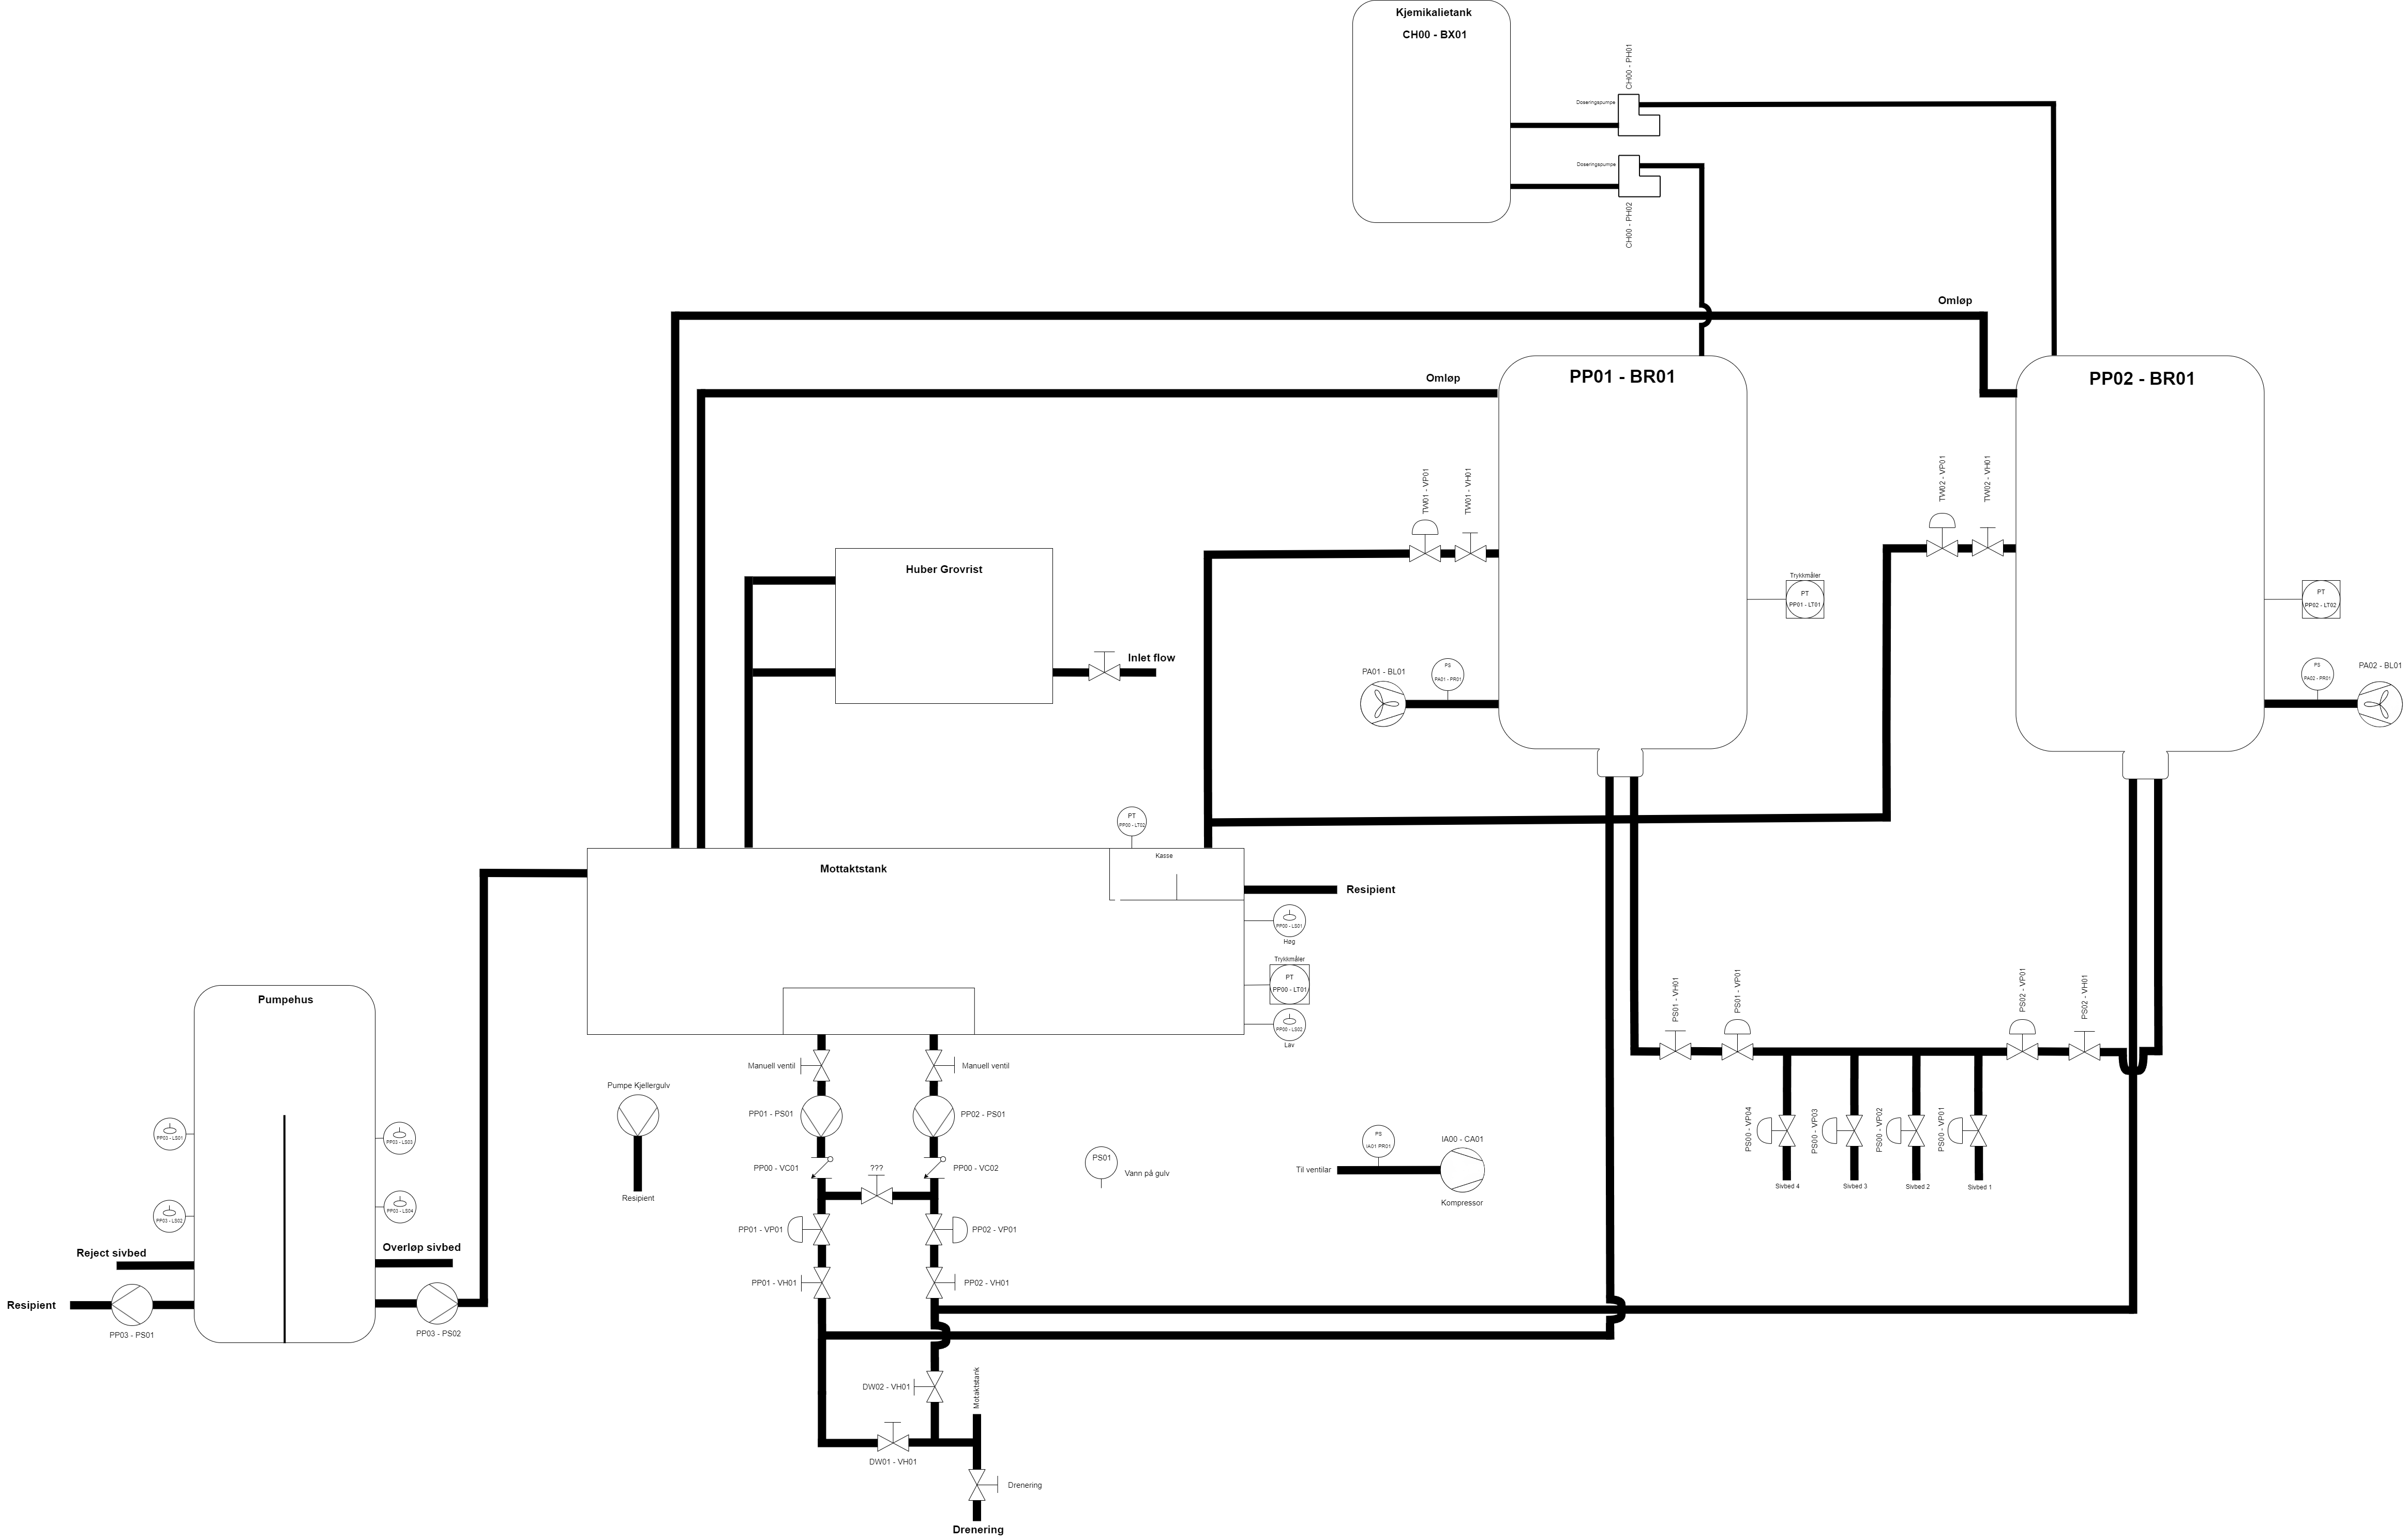
\includegraphics[angle=90,width=1\textwidth]{Figurar/PID.drawio.png}
    \caption{P\&ID}\label{fig:HMI}
\end{figure}
	\newpage
\section{Spesefikke anleggs forskjeller}
\thispagestyle{fancy}

Sjølv om Sande reiseanlegg anvender \gls{SBR}-teknologi så er det enkle spesefikke
punkter der dette reiseanlegget avviker ifrå normen. 
Sande reinseanlegg bruker eksempelvis ein spesiel form for slambehandling sett i norsk perspektiv.

Vanleg slambehandling i Noreg er oppsamling av slammet i tanker som handterast og tømmast av lokale etater.
På Sande blir ikkje slammet lagra, men jamnlig spreid ut over eit designert område. På dette området er
det planta siv som skal ta opp slammet og det resterande vatnet blir naturleg filtrert og drenert.
Desse områda kallast sivbed.

Sivbeda er konstruert med fleire dreneringslag som gjer at resterande vatn skiljast ut i designerte soner.
Her kan desse handterast vidare etter ønska behov. 
Grunna denne slambehandlingsmetoden er det på Sande reiseanlegg heller slamfjerning frå reaktor
i reaksjonsfasen. Dette blir gjort for å ha mindre konsentrert slam.

Sande reiseanlegg har fire sivbed og den kombinerte størrelsen er 676 kvadratmeter. Sivbeda er lokalisert på utsida av reiseanlegget.\newline
Videre har kvart sivbed sin eigen respektive ventil~\ref{fig:SivbedVentilar}, og under slambehandlinga vil kun ein ventil vere aktiv. 
 

\begin{figure}[htbp]
    \centering
    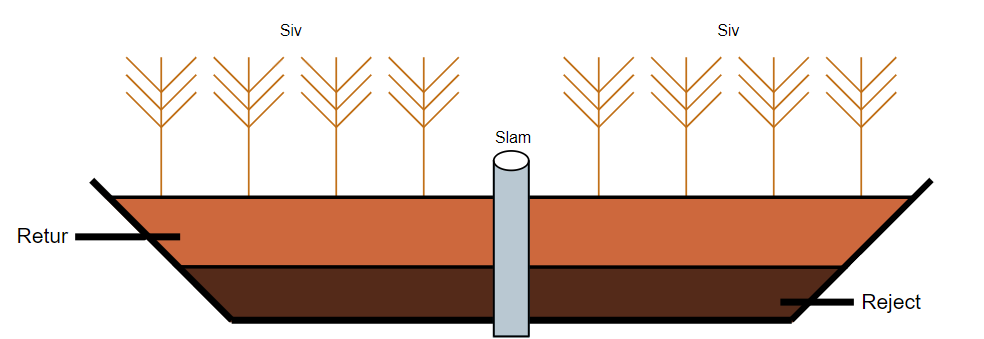
\includegraphics[width=1\textwidth]{Figurar/Sivbed.png}
    \caption{Illustrasjon sivbed}\label{fig:Sivbed}
\end{figure}

\newpage

Vatnet frå desse forskjellige dreneringslaga blir samla til eit pumpehus/komme.
Dette pumpehuset står ca femti meter ifrå sjølve reinseanlegget og er utstyrt med to pumper og nokre nivåbrytarar.
Pumpekommen er delt i to og skiller på vatnet som kjem ifrå dei forskjellige dreneringslaga.\newline
På Sande reiseanlegg er djupaste dreneringssona klassifisert som reinsa vatn (sivbed reject) og blir sendt ut til resepient.
Den øvre dreneringssona er forsatt klassifisert som skitten og blir returnert til mottakstanken. \newline \newline \newline \newline \newline

\begin{figure}[htbp]
    \centering
    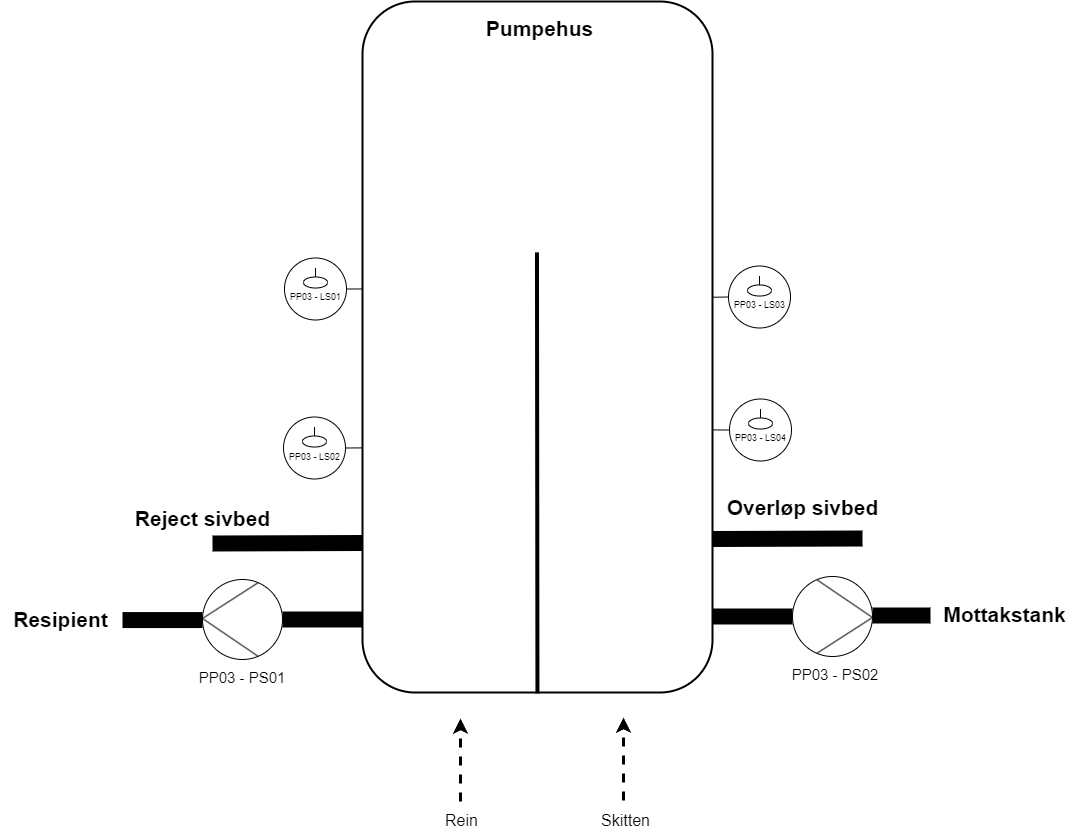
\includegraphics[width=1\textwidth]{Figurar/Pumpehus.drawio.png}
    \caption{P\&ID pumpehus}\label{fig:Pumpehus}
\end{figure}

\begin{figure}[htbp]
    \centering
    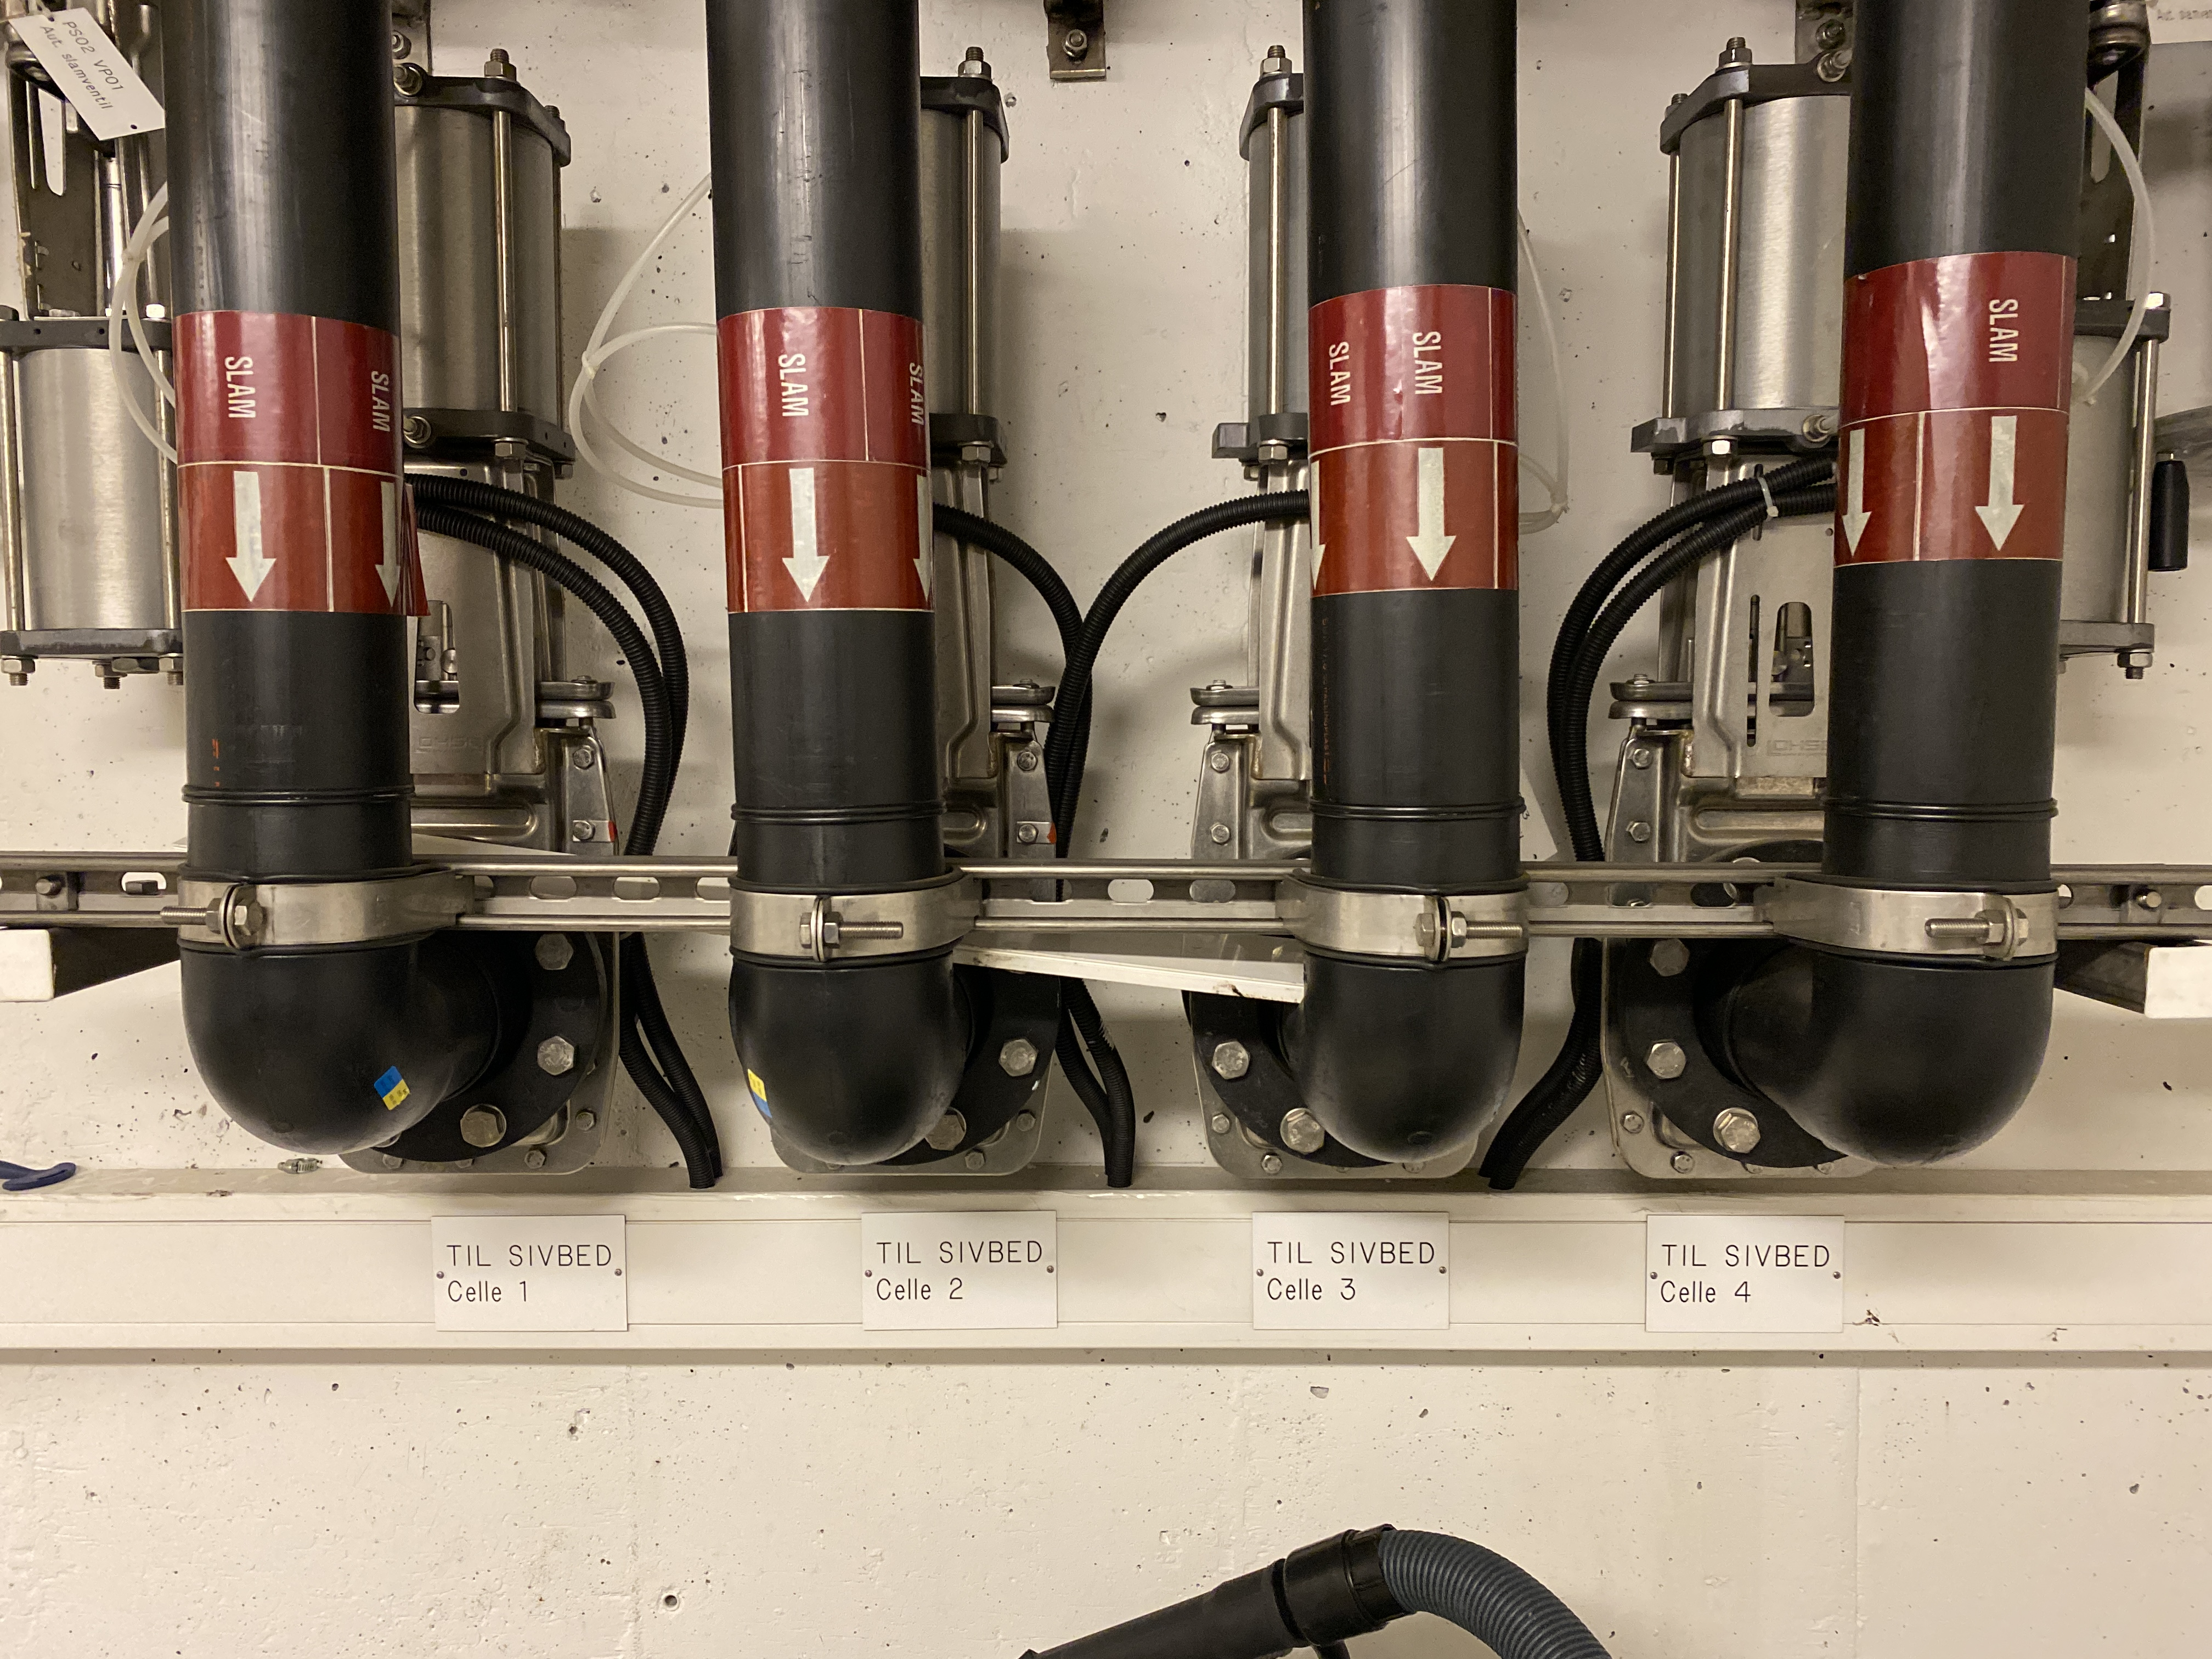
\includegraphics[width=1\textwidth]{Bilder/SivbedSande.jpg}
    \caption{Sivbed ventilar}\label{fig:SivbedVentilar}
\end{figure}

\newpage




	\newpage
\section{Dokumentasjon}
\thispagestyle{fancy}

Som tidlegare skildra i kapittel \ref{sec: 5} var ein stor del av oppgåva å dokumentere
verkemåten til anlegget. Vi bestemte oss for å gjere ei dokumentasjonsfornying
der vi henta inn alt det som var av tidlegare dokumentasjon og kombinerte det med vår nyerfarte kunnskap.

Vi oppretta ein funksjonsbeskrivelse som bygger vidare på driftsinstruksen (Vedlegg F) som var levert av 
Watercare i 2003. Dokumentet er tiltenkt ein slags bruksanvisning for heile anlegget,
der sikkerheit, prosess, verkemåte og styresystem er sentrale tema.

Funksjonsbeskrivelsen skal være forståeleg for alle intresserte parter og inneheld 
mange av våre nye figurar og avsnitt. Dokumentet innheld detaljert kvifor og korleis
ting heng saman og gir derfor ein forståelse av anlegget som ikkje var mogleg med den opphavlege dokumentasjonen.

Funksjonsbeskrivelsen inneheld alt om reinseanlegget på Sande men er delt opp i kapittel for å ikkje
overvelde lesar med unødvendig informasjon. Kompleksiteten auker gradvis gjennom dokumentet
og programmering av anlegget ligg under udjupa teknisk beskrivelse.

Dokumentet er delt opp i desse kapittela.

\begin{enumerate}
    \item Introduksjon
    \item Verkemåte
    \item Teknisk beskrivelse
    \item Drift og vedlikehald
    \item Feilsøking
    \item Utdjupa teknisk beskrivelse
    \item Teknisk underlag
\end{enumerate}

Alt som er nemnt her i kapittel 6 står meir detaljert under kapittel 3 i funksjonsbeskrivelsen og
er sentralt for å best forstå korleis anlegget fungerer.

Funksjonsbeskrivelsen ligg som vedlegg. (Vedlegg G)

	% Kapittel 7 - Tilrettelegging for programmering
	\chapter{Tillrettelegging for programmering}
\thispagestyle{fancy}
\label{sec:7} 

Som tidlegare beskrevet under kapittel \ref{sec: 5}, ynskte vi å bruke ei løysning som ikkje hadde høge lisenskostnadar for vår sluttkunde. 
Sunnfjord kommune var interessert å ikkje låse seg til ein fast leverandør, men heller ha moglegheita til å ha valet mellom fleire 
leverandørar innan \gls{PLS}. Dette ilag med moglegheiten til å utivde vår eigen kompetanse 
gjorde at vi såg vekk ifrå Siemens \gls{TIA}-portal \citep{Siemens}, som vi hadde lært igjennom \gls{PLS} emnet.
Programmet ynskte vi å skrive i strukturert tekst (\gls{ST}) men undersøkte også 
typar av grafiske diagrambaserte språk for å lettare vise samanhengar i programmet.

Det var også viktig at alle på gruppa kunne programmere samtidig og at ein felles programmeringsstandard skulle nyttast.
Det var viktig at parallelt arbeid ikkje skulle by på synkroniserings problem og at det fantest ei god løysning for dette.


	\section{IEC}
\thispagestyle{fancy}
\label{sec:5.2}


\gls{IEC} \citep{IEC} er ein internasjonal, ikkje statleg organisasjon som utviklar og publiserer tekniske standardar innan elektrofag. 
Norge er representert i \gls{IEC} ved Norsk Elektrotekniske Komité (\gls{NEK}) \citep{IEC-SNL}. 
\gls{IEC} har ein standard som dekker programmering av \gls{PLS} som går heilt tilbake til 1993\citep{Wiki-93}. 
Den nåverande standaren som omfamnar PLS er IEC 61131\citep{IEC-61131}. Dette er ein standard spesielt laga for programmerbare kontrollarar, og er delt opp i ti delar, der del tre tar for seg programmeringsspråk. 

Vårt program er i hovudsak tiltenkt programmert etter \gls{IEC} 61131-3 og \gls{IEC} \gls{PAS} 63131\citep{IEC-63131}. 
Der \gls{IEC} \gls{PAS} 63131 er ein standard utarbeida av \gls{IEC} som gir oss grunnlag for å lage \gls{SCD} samt å bruke forhandsdefinerte funksjonstemplater for funksjonsblokker. 
\gls{IEC} \gls{PAS} 63131 er laga med formål at leverandørindustrien og oljeselskap skal ha eit felles rammeverk for bruk på norsk sokkel, og er utarbeida etter NORSOK I-005:2013.
Ved å bruke desse standardane så gir det oss eit robust og fleksibelt rammeverk for å programmere anlegget. 
Ved bruk av dei forhandsdefinerte funksjonsblokkane har vi moglegheit til å enkelt knytte saman fleire delar av programmet vårt. 
Dette gir oss fleksibilitet ved å enkelt kunne endre og legge til funksjonar i programmet. 
Dette er noko vi har fokusert på, då vår oppdragsgivar har ytra eit ønskje om moglegheit for tilleggsfunksjonar i programmet. 
\newpage

	
	\section{Codesys}
\thispagestyle{fancy}
\gls{Codesys} \citep{Codesys} laga av \gls{Codesys} Group tilbyr ein open kjeldekodeløysning for prosjeket og har ingen lisenskostnadar. \citep{CodesysLisens}. 
I tillegg så kan prosjektfilane brukast på fleire typar PLS einingar \citep{CodesysPLS}. 
Dette gir vår oppdragsgivar fleksibilitet i korleis dei ønskjer å implementere vårt løysningsforslag til deira anlegg.

\gls{Codesys} nyttar programeringsspråkstandaren satt av \gls{IEC} 61131-3 som blant anna \gls{ST}, ``Sequential Function Chart'' (\gls{SFC}) og ``Ladder Diagram'' (\gls{LD}). 

\gls{Codesys} har nyleg fått støtte for integrering av \gls{github} i programvaren \citep{CodesysGIT}. 
Dette gjer det mykje enklare for oss å halde versjonskontroll
og enklare for gruppemedlem å programmere saman. 
\gls{github} har vi nytta på andre prosjekt og har vi god erfaring med.

Vidare så har \gls{Codesys} støtte for bibliotek igjennom \GLS{Codesys} Store \citep{CodesysStore}. 
Med å bruke kjende bibliotek så får vi tilgang til ei samling av gjenbrukbare kodeblokker, funksjonar og komponentar som vi kan nytte.
Dei biblioteka vi ønskjer å bruke er som følgjer:

\begin{itemize}
    \item \GLS{Codesys} Building Automation \citep{BuildingAutomation}
    \item SysTime \citep{DateAndTime}
    \item Util \citep{Util}
\end{itemize}


\newpage

	\section{SCD}
\thispagestyle{fancy}

Etter vi hadde valt dei blokkene vi ønskte var det naturleg å sette seg ned å planlegge korleis vi ønska å knytte desse blokkene opp i mot anlegget. 
Vi valte da å starte med å lage eit System Control Diagram (SCD) over anlegget. 
SCD er ein grafisk representasjon av anlegget, som visar komponentane i anlegget og deira funksjon, forbindelsar og struktur. 
IEC PAS 63131 standaren gir oss retningslinjene for utforming av diagrammet.


\begin{figure}[htbp]
    \centering
    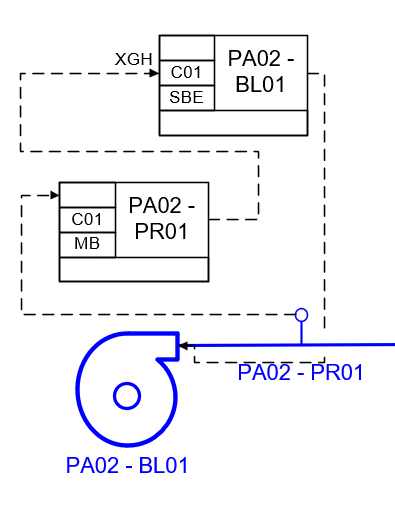
\includegraphics[width=0.35\textwidth]{Bilder/Visio_eksempel.png}
    \caption{Utsnitt frå SCD}\label{fig:SCD eksempel}    
\end{figure}


Første utkast av vårt SCD inneheldt koplingane frå komponentar til blokker og korleis forbindelsane imellom desse skulle fungere. 
Korleis dei forskjellige sekvensane skulle interagere med blokkene og komponentane våre var litt uklart for oss på detta stadiet,
så vi valde å gå vidare med å lage noko av programmet, slik at vi lettare kunne danne oss eit bilete av korleis vi ville løyse oppgåva.
Når skalet av programmet var laga, kunne vi fullføre SCD. Vi hadde da 



\newpage
	\section{Tilstandsmaskin}
\thispagestyle{fancy}

Vi identifiserte tidleg i prosessen at vi hadde eit ønskje om å lage ein tilstandsmaskin som hadde den 
overordna styringa over kvar reaktor. 
Sidan ein SBR tank er prinsipielt oppbygd av forskjellige sekvensar, virka det logisk å lage til ein 
tilstandsmaskin som gjekk igjennom dei forskjellige tilstandane basert på logikk som vart plassert i dei forskjellige tilstandane. 
Med erfaringane vi hadde danna oss om anleggets verkemåte 
kunne vi enkelt tenke oss ei tilstandsmaskin som vart intregert mot dei forskjellige sekvensane i anlegget. 
Tilstandsmaskina tar inn signal i frå dei forskjellige tilstandane i anlegget og avansera til neste 
sekvens når logikken i tilstanden gir signal om at den er ferdig. 


\begin{figure}[htbp]
    \centering
    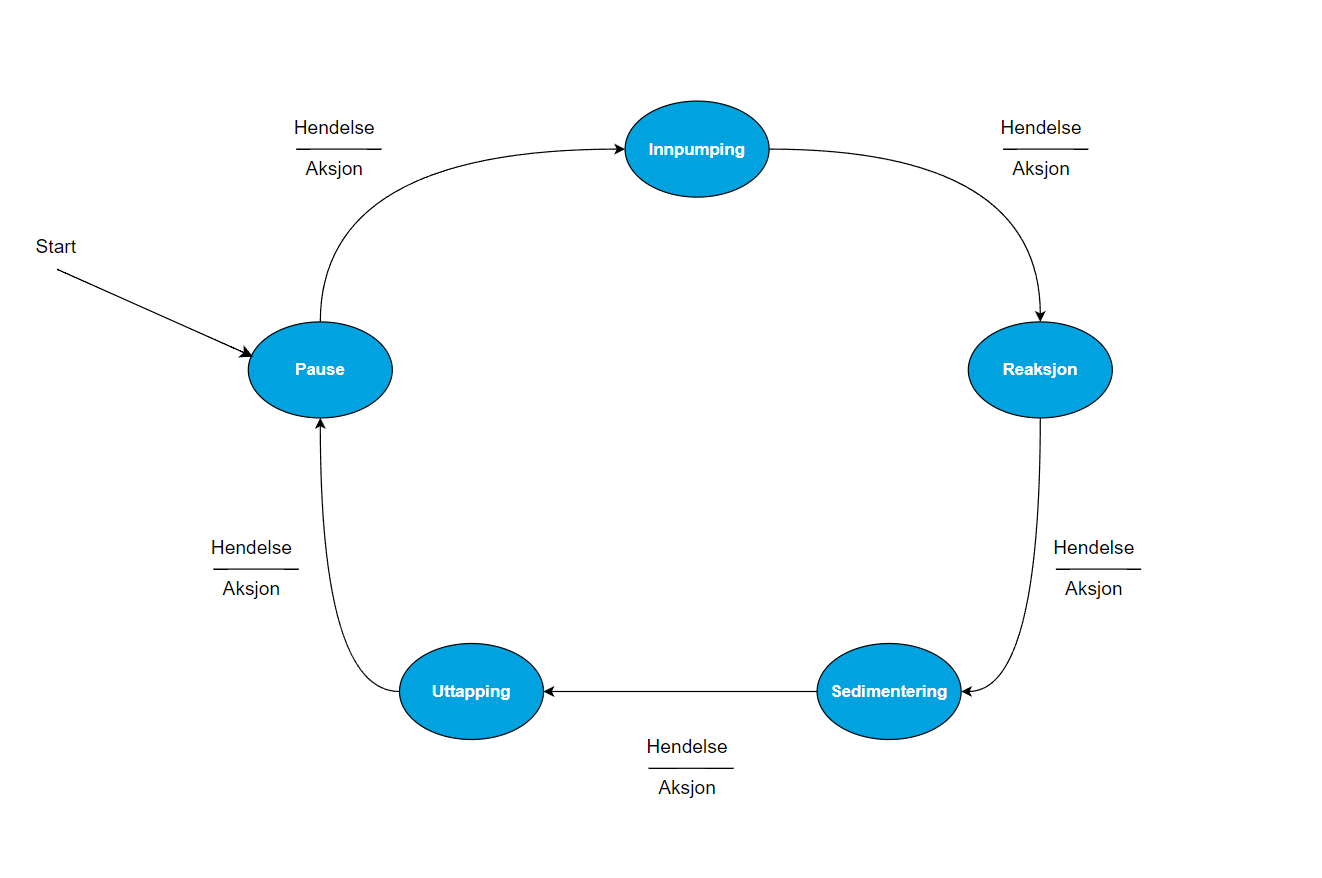
\includegraphics[width=1\textwidth]{Figurar/Tom tilstandsmaskin.png}
    \caption{Tilstandsmaskin prinsipp}\label{fig:Tilstandsmaskin prinsipp}    
\end{figure}

\newpage



	% Kapittel 8 - Programmering
	\chapter{Programmering}
\thispagestyle{fancy}
Etter å ha danna oss eit godt grunnlag og eit bilete av korleis vi ønska programmet i kapittel \ref{sec:5} 
begynte vi med programmeringa med eit tomt prosjekt i \gls{Codesys}. Første steget i var å 
settje oss inn i, og programmere \gls{IEC} blokkene som vi valgte i kapittel \ref{sec:5.2}

%% CODESYS is a software platform for industrial automation technology. 
%%The core of the platform is the IEC-61131-3 programming tool "CODESYS Development System".


	\section{IEC funksjonsblokker} \label{IEC Seksjon}
\thispagestyle{fancy}

Vi gjorde eit utval av moglege funksjonsblokktemplat basert på dei komponentane vi identifiserte i reinseanlegget.
For å lage eit robust program valde vi å fokusere på to inngangsfunksjonar, \gls{MA}, \gls{MB}, og to utgangsfunksjonar \gls{SBE}, \gls{SBV},
som måtte programmerast frå grunn. 

Funksjonsblokktemplata inneholdt avanasert funksjonalitet som vi visste ville ta lang til å programmere.
Sjølv om ikkje all denne funksjonaliteten var naudsynt for reinseanlegget,
valde vi likevell å programmere alt, ettersom blokkene gir potensiell meirverdi i mogleg utvidning og eventuell bruk i andre styresystem.
Det gav oss også ein tydleg retning å arbeide mot og vi visste at blokka ville dekke alle aktuelle behov.

\gls{IEC} har sentrale begrep som vi ønskjer å utdjupe nærmare. Grunna mangel på gode norske begrep
og for å forhindre forvirring vel vi å beskrive begrepa slik dei er skildra i normen \citep{IECGlossery}

\begin{itemize}
    \item \textbf{Lock:} Action overruling any other signal while being true
    \item \textbf{Force:} Action overruling any other signal                        
    \item \textbf{Disable transition:} Transition high/low function not avaliable  
    \item \textbf{Blocking:} Prevention of certain functions or operations          
    \item \textbf{Suppression:} Disable alarm annunciation as well as any associated automatic actions
\end{itemize}
Det er også andre genrelle forkortingar som er viktige i skildring av desse blokkene.
\begin{figure}[htbp]
    \centering
    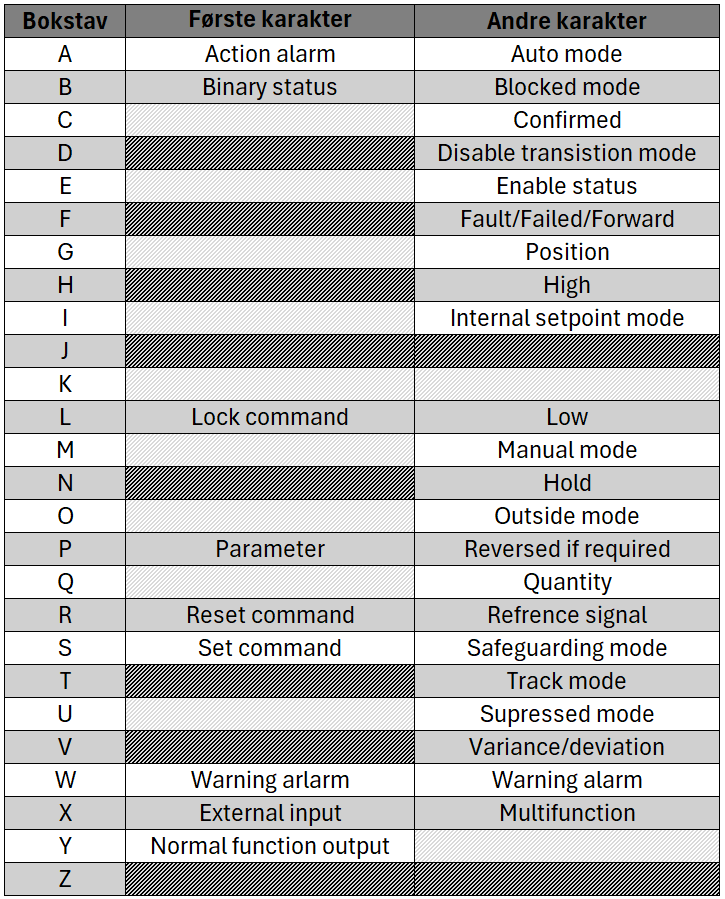
\includegraphics[scale=0.33]{Figurar/IEC bokstavmatrise.png}
    \caption{Bokstavmatrise basert på Table A.1 i \gls{IEC} \gls{PAS} 63131:2017 \citep{A1}}\label{fig:SBE tilstandsmaskin}
\end{figure}

\newpage

\subsection{Monitor Binary}
Inngangsfunksjon \gls{MB} blir nytta til automatisk overvaking, alarmhandtering, framvising og låsing av binære prosessvariablar \citep{IEC-63131}.
Funksjonsblokka er nytta i programmet for å overvake alle digitale inngangar t.d. pressostat og nivåvipper.

\gls{MB} mottar binær verdi på X og returnerer verdi på Y. \newline
Denne utgangsverdien har moglegheit for tidsforseinking, invertering, låsning, ``blocking'' og ``suppression'' via ``force'' inngangsvariablar og parameter.

Blokka har tre statusvariablar som indikerer modus og område (BU, BB, BX), ein utgang for indikasjon av feil (YF) med moglegheit for ``suppression''
og ein inngang (RX) for reset av eventuell låst verdi. \newline 

\begin{figure}[htbp]
    \centering
    \begin{subfigure}[b]{1\textwidth}
        \centering
        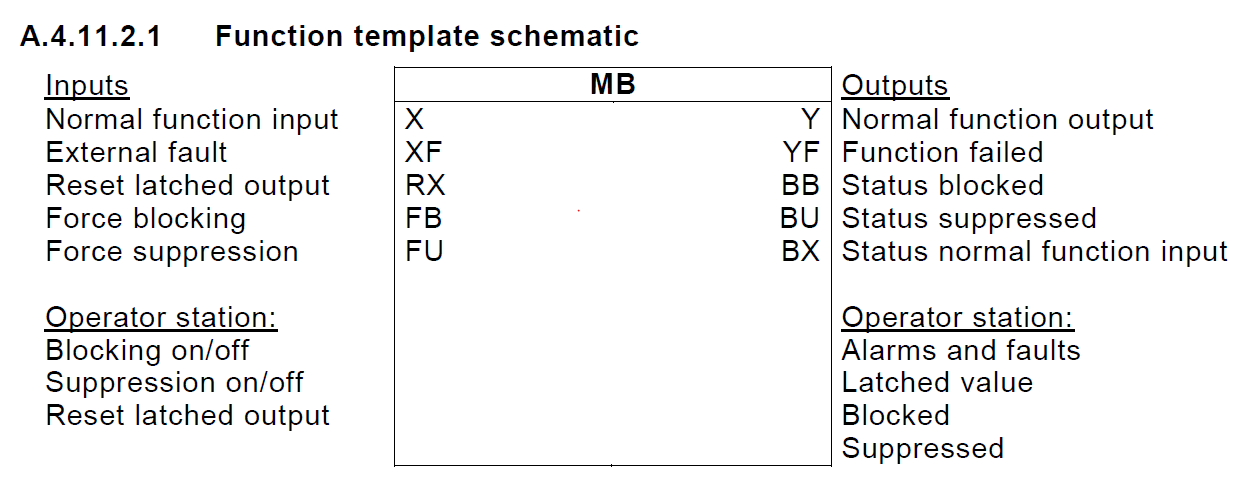
\includegraphics[width=0.7\textwidth]{Bilder/MBBlokkIEC.png}
        \caption{\gls{IEC} \gls{PAS} 63131:2017 \citep{MB}}\label{fig:Monitor Binary blokk IEC}
    \end{subfigure}
    \hfill
    \begin{subfigure}[b]{1\textwidth}
        \centering
        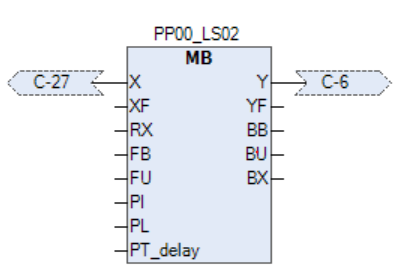
\includegraphics[width=0.5\textwidth]{Bilder/MBBlokkIProgrammet.png}
        \caption{MB nytta i programmet}\label{fig:Monitor Binary blokk i programmet}
    \end{subfigure}
    \caption{Monitor Binary}\label{fig:Monitor Binary}
\end{figure}

Meir informasjon om blokka, inngangar, utgangar, og parameter er tilgjengeleg i vedlegg. (Vedlegg C.1)

\newpage

\subsection{Monitor Analogue}
Inngangsfunksjon \gls{MA} er nytta for skalering, visning, overvaking og alarmhandtering av
analoge prosess og kontrollvariablar \citep{IEC-63131}.
Funksjonsblokka er nytta for å overvake analoge trykknivågivarar, 
og å skalere og vise desse som ein fyllingsgrad i prosent.

\gls{MA} hentar rå analog verdi på X og returnerer verdi på Y.
Denne utgangsverdien blir skalert basert på parameter og har hysterese og dødband tilgjengeleg.

Hysterese og dødband definerer områder rundt eit gitt setpunkt der systemet 
ikkje endrar tilstand eller reagerer på små variasjonar.
Dette gjer at systemet unngår hyppige vekslingar og unødvendige justeringar.

Funksjonsblokka har to forvarsel (WH og WL) og to handlingar med alarm (AHH og ALL).
Det er moglegheit for tidsforsinking, ``blocking'' og ``suppression'' av desse via ``force'' inngangsvariablar og parameter.

Blokka har fem statusvariablar som indikerer modus og område (BU, BB, BHH, BLL, BBLL, BBHH), ein utgang for indikasjon av feil (YF)
og fire hendingar (BXHH, BXH, BXLL, BXL) utan ``blocking'' og ``suppression'' som nyttast for styring.

Grenser på varsling og hendigar er justerbare via parameter.

\begin{figure}[htbp]
    \centering
    \begin{subfigure}[b]{0.49\textwidth}
        \centering
        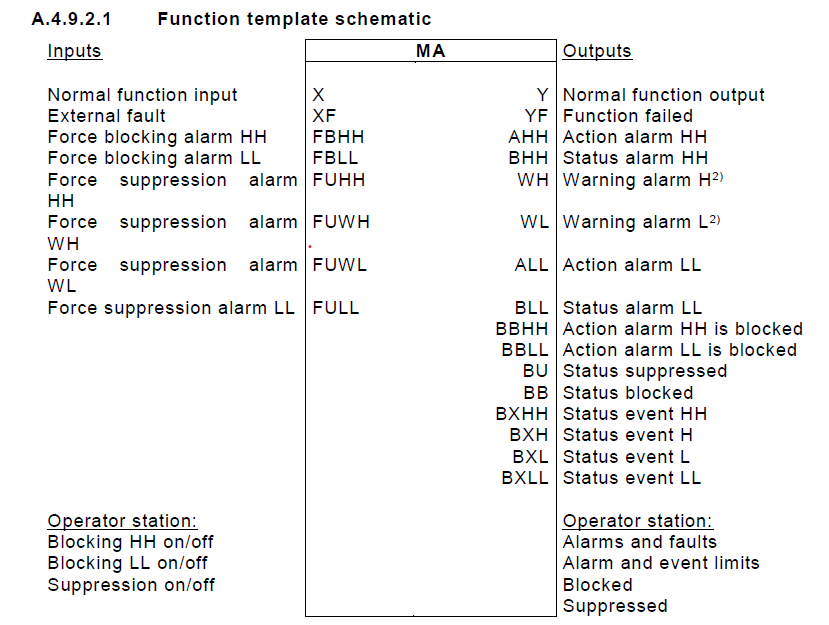
\includegraphics[width=1\textwidth]{Bilder/MABlokkIEC.png}
        \caption{\gls{IEC} \gls{PAS} 63131:2017 \citep{MA}}\label{fig:Monitor Analogue blokk IEC}
    \end{subfigure}
    \hfill
    \begin{subfigure}[b]{0.49\textwidth}
        \centering
        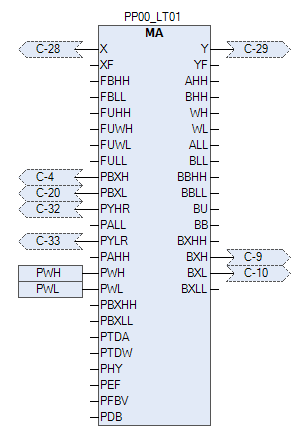
\includegraphics[width=0.7\textwidth]{Bilder/MABlokkIProgrammet.png}
        \caption{MA nytta i programmet}\label{fig:Monitor Analogue blokk i programmet}
    \end{subfigure}
    \caption{Monitor Analogue}\label{fig:Monitor Analogue}
\end{figure}

Meir informasjon om blokka, inngangar, utgangar, og parameter er tilgjengeleg i vedlegg. (Vedlegg C.2)

\newpage

\subsection{Switch Binary Electrical} 

Utgangsfunksjon \gls{SBE} blir nytta for binærkontroll (av/på) av strøymingselement for elektrisitet, varme eller væske. 
Den kontrollerte komponenten kan vere t.d. motor, pumpe, varmeelement, vifte \citep{IEC-63131}. \newline
Funksjonsblokka er nytta til å styre motorar, pumper og blåserar. (Vedlegg C.3)

Funksjonsblokka har tre modus, auto, manuell og lokal. Lokal betyr lokal HMI eller direktekøyring.
\gls{SBE} hentar start/stopp signal på
\begin{enumerate}
    \item \textbf{Auto:}        XH og XL  
    \item \textbf{Manuell:}     HMI
    \item \textbf{Lokal:}       XOH og XOL
\end{enumerate}
Aktiveringssignal er tilgjengeleg via inngang XE. \newline
Blokka sender køyrsignal på Y og via pulsmodulerte utgangar YH og YL.

\gls{SBE} inneheld ei tilstandsmaskin med fire funksjonstilstandar. 
\begin{enumerate}
    \item \textbf{Høg:}                 Komponent køyrer
    \item \textbf{Lav:}                 Komponent stoppa
    \item \textbf{Transisjon mot lav:}  Fått stoppsignal
    \item \textbf{Transisjon mot høg:}  Fått køyrsignal.
\end{enumerate}

I transisjonstilstand ventar blokka på eksternt tilbakemelding (XGH) 
og sett tilstanden til høg/lav etter at korrekt tilbakemelding er mottatt.
Dette vises også via to statusvariablar (BCL, BCH)

Blokka har sju andre statusvariablar som indikerer modus og område (BA, BO, BS, BB, BU, BXH, BXL) og
ein utgang for indikasjon av feil (YF) med tilhøyrande heiltallsverdi (YFI) som indikerer feiltype. \newline
Feilstatus har moglegheit for ``suppression''.

Blokka har fire signal for høg/lav tvangskøyring, der ``lock'' endrar modus til maneull (LSH, LSL) og ``force'' gjer ikkje (FSL, FSH)
og to signal for høg/ lav ``force disable transition'' (FDH, FDL).
Desse signala har moglegheit for ``blocking''.

\newpage

\begin{figure}[htbp]
    \centering
    \begin{subfigure}[b]{0.46\textwidth}
        \centering
        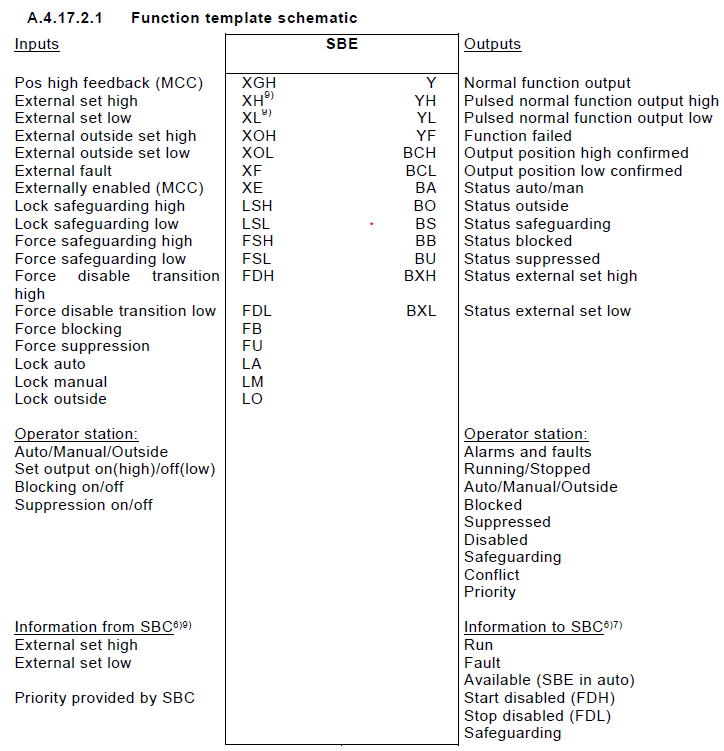
\includegraphics[width=1\textwidth]{Bilder/SBEBlokkIEC.png}
        \caption{\gls{IEC} \gls{PAS} 63131:2017 \citep{SBE}}\label{fig:Switch Binary Electrical blokk IEC}
    \end{subfigure}
    \hfill
    \begin{subfigure}[b]{0.46\textwidth}
        \centering
        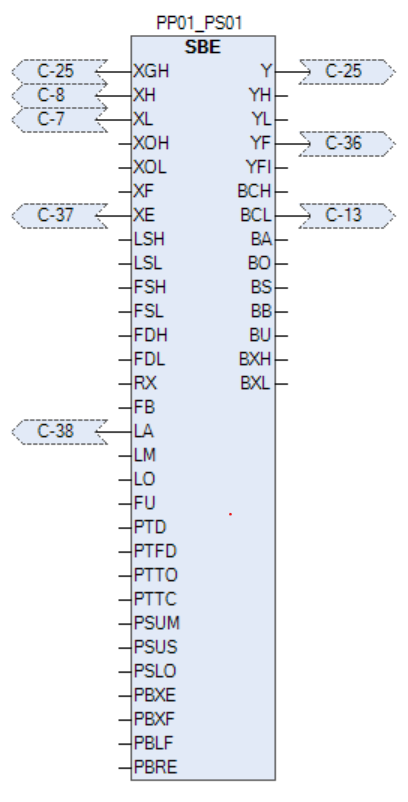
\includegraphics[width=0.5\textwidth]{Bilder/SBEBlokkIProgrammet.png}
        \caption{SBE nytta i programmet}\label{fig:Switch Binary Electrical blokk i programmet}
    \end{subfigure}
    \caption{Switch Binary Electrical}\label{fig:Switch Binary Electrical}
\end{figure} 
\begin{figure}[htbp]
    \centering
    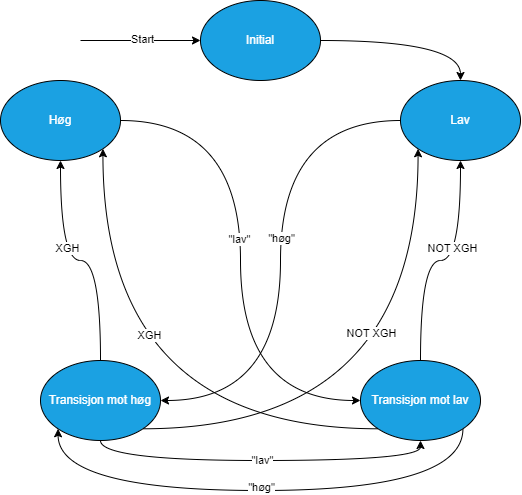
\includegraphics[scale=0.45]{Figurar/SBE.drawio.png}
    \caption{Prinsippskisse SBE tilstandsmaskin standard parameteroppsett}\label{fig:SBE tilstandsmaskin}
\end{figure}
Meir informasjon om blokka, inngangar, utgangar, og parameter er tilgjengeleg i vedlegg. (Vedlegg C.3)
\newpage
\subsection{Switch Binary Valve}

Utgangsfunksjon \gls{SBV} skal nyttast til binær (av/på) kontroll av eit strøymingselement ved å endre strøymen av medium (varme eller væske). 
Typisk komponentar som styrast er bl.a. ventilar og spjeld \citep{IEC-63131}.
Funksjonsblokka er i nytta til å styre ventilar.

Samanlikna med \gls{SBE} har \gls{SBV} har tre modus, auto, manuell og lokal som nyttar inngagnar med same namn.
\gls{SBV} hentar opne/stenge signal på
\begin{enumerate}
    \item \textbf{Auto:}        XH og XL  
    \item \textbf{Manuell:}     HMI
    \item \textbf{Lokal:}       XOH og XOL
\end{enumerate}
Blokka sender signal på Y og via pulsmodulerte utgangar YH og YL.

\gls{SBV} inneheld ei tilstandsmaskin med fire funksjonstilstandar. 
\begin{enumerate}
    \item \textbf{Høg:}                 Komponent open
    \item \textbf{Lav:}                 Komponent stengd
    \item \textbf{Transisjon mot lav:}  Fått stengesignal
    \item \textbf{Transisjon mot høg:}  Fått opnesignal.
\end{enumerate}

I transisjonstilstand ventar blokka på eksternt tilbakemelding (XGH, XGL) 
og sett tilstanden til høg/lav etter at korrekt tilbakemelding er mottatt.
Dette vises også via to statusvariablar (BCL, BCH)

Blokka har fem andre statusvariablar som indikerer modus og område (BA, BO, BS, BB, BU) og
ein utgang for indikasjon av feil (YF) med tilhøyrande heiltallsverdi (YFI) som indikerer feiltype. \newline
Feilstatus har moglegheit for ``suppression''.

Blokka har fire signal for høg/lav tvangskøyring, der ``lock'' endrar modus til manuell (LSH, LSL) og ``force'' gjer ikkje (FSL, FSH)
og to signal for høg/ lav ``force disable transition'' (FDH, FDL).
Desse signala har moglegheit for ``blocking''.

\newpage

\begin{figure}[htbp]
    \centering
    \begin{subfigure}[b]{0.45\textwidth}
        \centering
        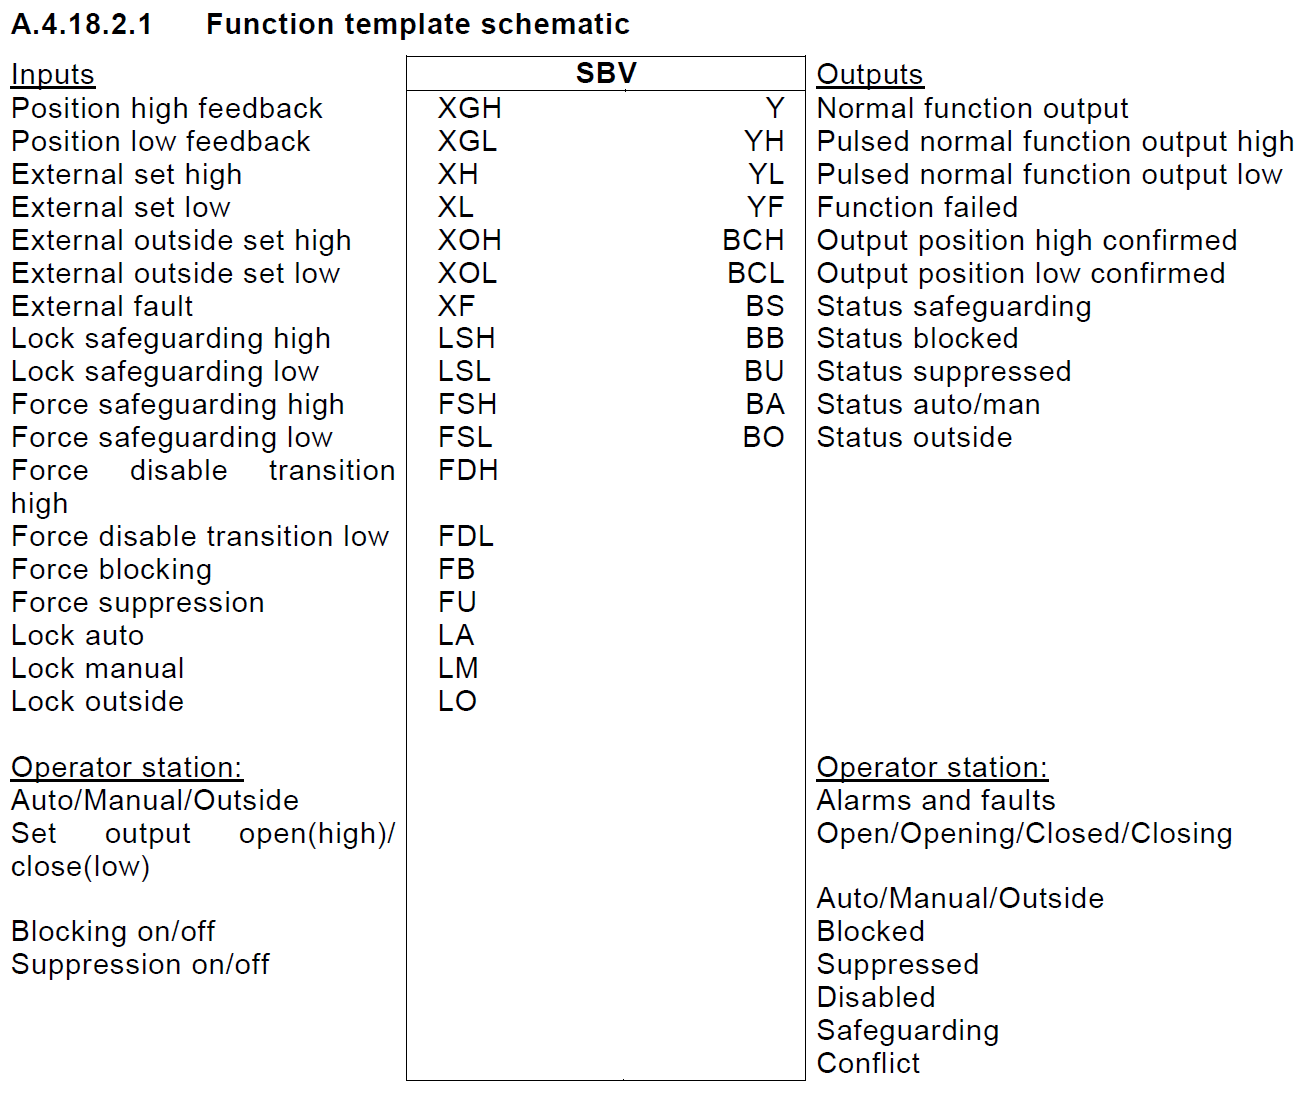
\includegraphics[width=1\textwidth]{Bilder/SBVBlokkIEC.png}
        \caption{\gls{IEC} \gls{PAS} 63131:2017 \citep{SBV}}\label{fig:Switch Binary Valve blokk IEC}
    \end{subfigure}
    \hfill
    \begin{subfigure}[b]{0.45\textwidth}
        \centering
        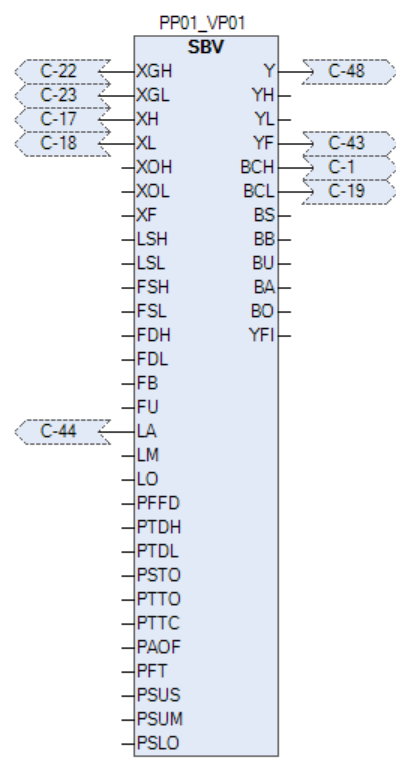
\includegraphics[width=0.5\textwidth]{Bilder/SBVBlokkIProgrammet.png}
        \caption{SBV nytta i programmet}\label{fig:Switch Binary Valve blokk i programmet}
    \end{subfigure}
    \caption{Switch Binary Valve}\label{fig:Switch Binary Valve}
\end{figure}
\begin{figure}[htbp]
    \centering
    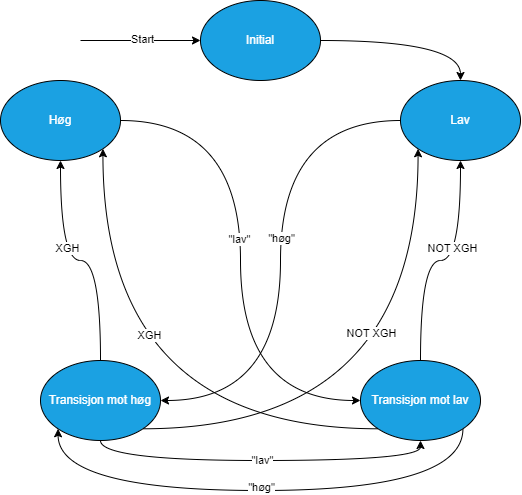
\includegraphics[scale=0.47]{Figurar/SBE.drawio.png}
    \caption{Prinsippskisse SBV tilstandsmaskin standard parameteroppsett}\label{fig:SBV tilstandsmaskin}
\end{figure}


Meir informasjon om blokka, inngangar, utgangar, og parameter er tilgjengeleg i vedlegg. (Vedlegg C.4)

\newpage


%\begin{figure}[htbp]
%    \centering
%    \begin{subfigure}[b]{0.45\textwidth}
%        \centering
%        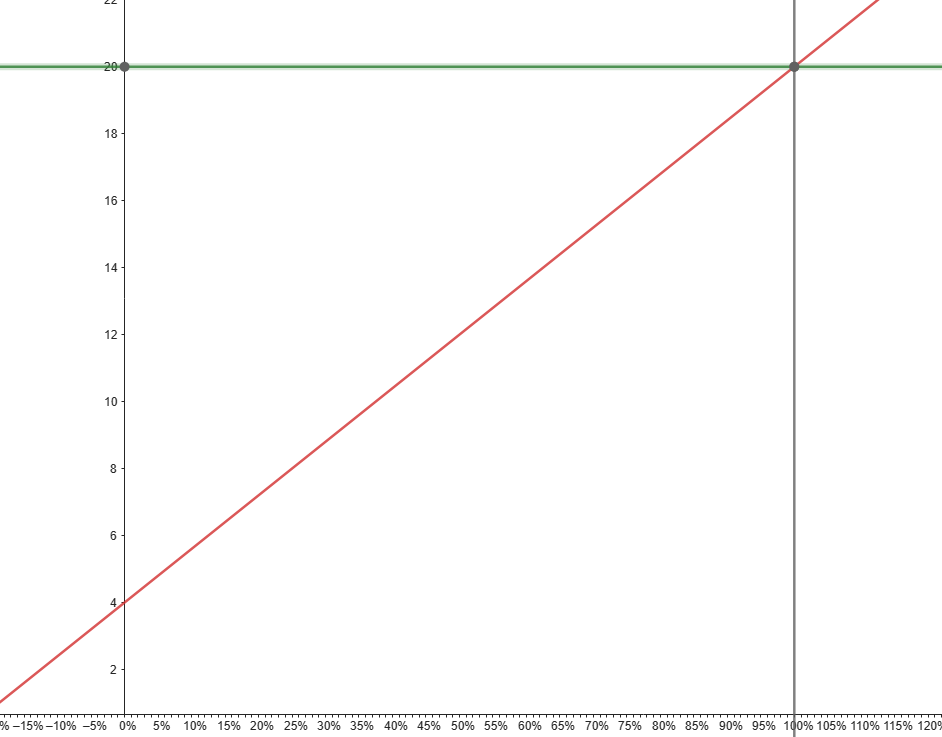
\includegraphics[width=1\textwidth]{Bilder/4_20mA_Scaling.png}
%        \caption{Skalering av mA mot prosent}\label{fig:Skalering av mA mot prosent}
%    \end{subfigure}
%    \hfill
%    \begin{subfigure}[b]{0.45\textwidth}
%        \centering
%        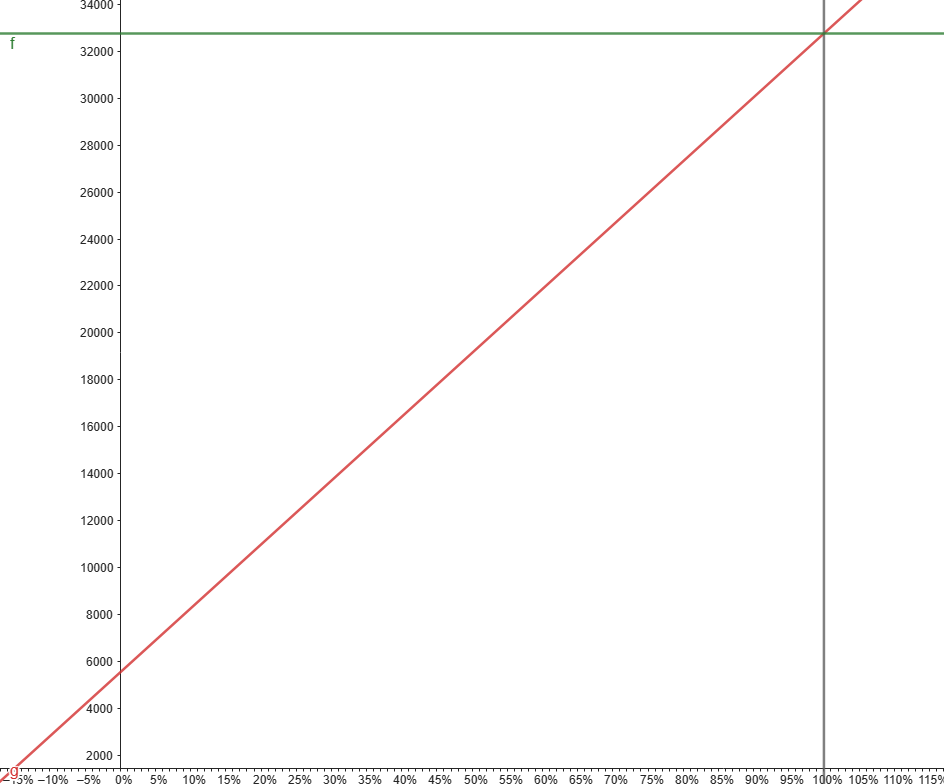
\includegraphics[width=0.95\textwidth]{Bilder/27327_prosent_Scaling.png}
%        \caption{Skalering av prosent til verdi}\label{fig:Skalering av prosent til verdi}
%    \end{subfigure}
%    \caption{Dei forskjellige skaleringane av inngangssignal}\label{fig:Skalering av prosent til verdi}
%\end{figure}



	\section{Generelle funksjonsblokker}
\thispagestyle{fancy}

% Legge inn forklaring av "felleskoden", utrekningar', sivebedrotasjon', dataprossesing', Høgbelastningsprogram', ProvessedWater.
% Alt under her er er ikkje skrevet i stein.

Undervegs i programmeringa av \gls{IEC} blokkene såg me også nødvendigheita av nokon generelle funksjonsblokker
som kunne gjenbrukast fleire gonger i programmet. Dette er då hensiktsmessigt sidan ein då slepp og skrive lik 
funksjonalitet fleire gonger, men heller kallar ei \gls{FB} som kann gjere denne same jobben.

\subsection{fbTimer}
Timer (Sjå appendix xXx) \gls{FB} kan brukast om ein treng ein tids forseinking i programmet.
Her kan ein nytta tidsforsinka inn, tidsforsinka ut eller ein kombinasjon av begge.

\subsection{fbAnalougeAlarm}
Analogue alarm (sjå appendix xXx) \gls{FB} brukast til å overvåke, tidsforsinke, behandle grenser, 
gje alarmar og legge på hystereser på ferdig skalerte analoge inngangsverdiar.

\subsection{fbDigitalAlarm}
Digital alarm (Sjå appendix xXx) \gls{FB} kan overvåke, tidsforsinke og gje alarmer. Det er valbart om blokka skal trigge på høg eller låg
inngang basert på ein parameter.

\subsection{fbSwap}
Swap \gls{FB} (sjå appendiksar) får ein inngangsverdi og sekvensielt bytter på og bruke to utgangsverdiar. Det vil sei at blokka hugsar på kva utgang som vart brukt sist,
og vil bruke den andre utgangen ved neste kall. Blokka har også moglegheit for feilhandtering.

\subsection{fbCalculations}
Calculations \gls{FB} (Sjå appendiks xXx) gjer nokre rekneoppgåver som ligger i bakgrunnen og køyrer kontinuerleg. 
Det er i hovudsak utrekningar av volum i reaktor, mottakstank og drenert volum i frå reaktortank.

\subsection{fbTimeMeter}
Time meter \gls{FB} (Sjå appendiks xXx) er ei blokk som teller tid så lenge den blir kalla på og lagrar desse verdien i forskjellige tidsformater.
Denne er brukt i programmet til å telle gangtid for forskjellige eletriske komponentar.

\subsection{fbHighLoad}
High Load \gls{FB} (Sjå appendiks xXx) lokka blir brukt til og overvåke antatt innstraumning i mottakstanken basert på nivå endringa i tanken. 
Blokka kalkulerar gjennomsnittleg tilstraumning ved å sample tank nivået kvart minutt over totalt 30 minutt.
Denne kalkuleringa blir samanlikna med eit parameter PXR 'setpunkt' for å sette annlegget i høgsbelastningsmodus.
Blokka gjer også antatt tilstrøymning per time.

\subsection{fbSivbedRotation}
Anlegget har fire ventilar til sivebedet som det er viktig å oppretthalde rotasjon imellom. Anlegget tappar frå ein reaktor om gongen, 
og \gls{FB} Sivbedrotation vel kva ventil som skal aktiverast.
Rotasjon blir angitt av ein parameter som fastset kor mange syklusar kvar ventil skal nyttast. 
Det er også mogleg å ta ein ventil ut av rotasjonen, slik at den ikkje blir inkludert i syklusen.

\subsection{fbDataprocessing}
fbDataprocessing (Sjå appendiks xXx) blir brukt i samband med innsamling av driftsdata. 
Når nokon av objekta som er tiltenkt å ha driftsdata køyrer eller er aktive, blir desse sendt til fbDataprocessing, og derifrå kallar den opp fbTimeMeter som lagrar og teller driftsdata for objektet.

\subsection{fbProcessedWater}
fbProcessedWater (Sjå appendiks xXx)
Det er laga ei eiga blokk for å halde oversikt over driftsdata som omhandlar behandla vann for anlegget. 
Denne blokka gir informasjon for totalt behandla vann, nåverande år, nåverande månad, nåverande veke, nåverande dag, førre år, færre månad, færre veke og førre dag.
	\section{Tilstandsmaskin}
\thispagestyle{fancy}

Etter at \gls{IEC} blokkene var ferdige, byrja vi på tilstandsmaskina som skulle styre sjølve \gls{SBR}-prosessen. 
Vi hadde allereie danna oss eit bilete, men kunne no byrja å bruke kunnskapen frå verkemåten til anlegget
til å grovt fylle inn dei hendelsane og aksjonane som foregikk mellom tilstandsendringar. 
Tilstandsmaskina er bygd opp av dei fem reaktortilstandane som eksisterar i eit \gls{SBR}-anlegg.

Dette er ein enkel modell av korleis tilstandsmaskina er programmert men gir eit godt innblikk i systemet.

\begin{figure}[htbp]
    \centering
    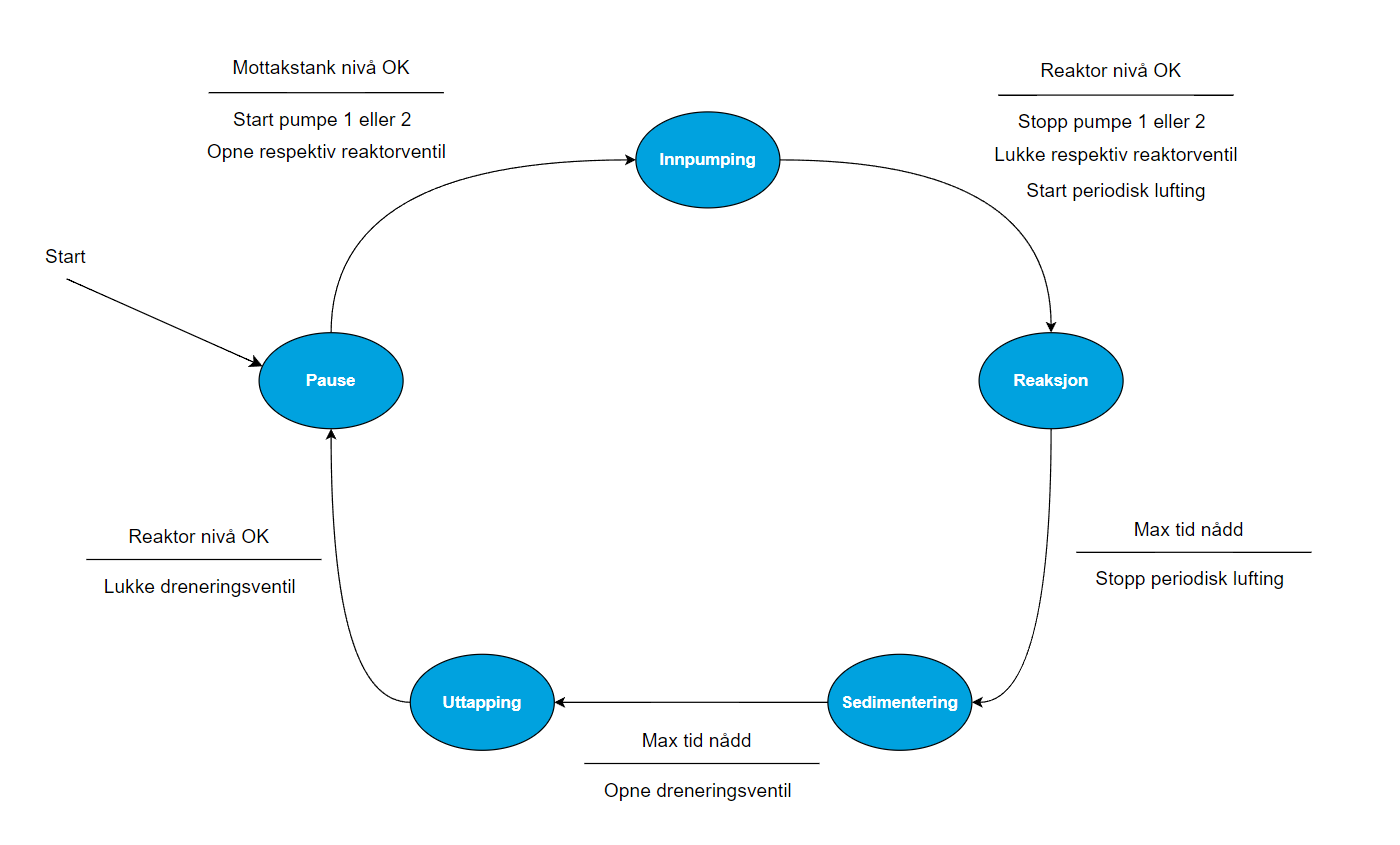
\includegraphics[width=1\textwidth]{Figurar/Simpel tilstandsmaskin.png}
    \caption{Enkel model av tilstandsmaskin}\label{fig:SimpelTilstandsmaskin}
\end{figure}

Utifrå det vi allereie hadde lært om anlegget visste vi kva inngangssignal og logikk som ville gi
``Mottakstank nivå OK'' og la tilstandsmaskina avansere ifrå pause til innpumping. Denne jobben utførte vi ved å lage ei
funksjonsblokk for kvar tilstand (tilstandslogikk) der aktuell inngang, utgang og logikk skulle samlast.

\newpage

I sjølve programmeringa av tilstandsmaskina blei den oppretta som ei eiga funksjonsblokk, noko som gav oss moglegheita å bruke den for begge reaktorane.
Tilstandsmaskina er laga med fem inngangar og seks utgangar, og baserer seg på ``switch/case'' logikk.

Tilstandsmaskina sender ut høg på den respektive utgangen som samsvarer med reaktortilstanden den er i. Dersom tilstandsmaskina får tilbake
OK signal på den respektive tilstandsinngangen avanserer tilstandsmaskina.
Det er også mogleg å hente ut kva aktiv tilstand ved hjelp av ein integer verdi (1-5)

\begin{figure}[htbp]
    \centering
    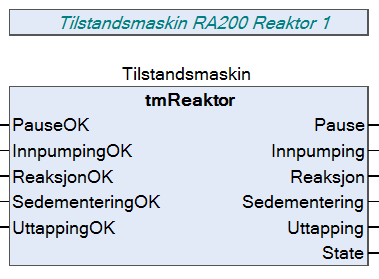
\includegraphics[width=0.4\textwidth]{Bilder/Tilstandsmaskin.png}
    \caption{Tilstandsmaskin implementert i programmet}\label{fig:TilstandsmaskinIProgram}
\end{figure}



	\newpage
\section{Tilstandslogikk}
\thispagestyle{fancy}

Styring og logikk som skulle skje i kvar tilstand valgte vi å samle i ei funksjonsblokk som vi kaller tilstandslogikk og som fikk navn etter tilstanden
den skulle styre. Desse funksjonsblokkene er skrevet og løyst spesefikt for deira arbeidsoppgåver i programet og kvar
tilstand har eigen funksjonsblokk med tilstandslogikk. \newline
Kvar tilstandslogikk får inn XE (external enable) ifrå tilstandsmaskina som startar tilstandslogikken. Når sekvensen er ferdig sender
funksjonsblokka høg på utgang Y som returerast til tilstandsmaskina som avanserer til neste tilstand og tilstandslogikk.

Det er tilstandslogikken som har ansvar for å samarbeide med IEC-blokkene som vidare
leser inngangssignal, startar og stoppar elektrisk utstyr, kontrollerer feedback, feilmeldingar og skriv akutelle parameter.

\begin{figure}[htbp]
    \centering
    \begin{subfigure}[b]{0.3\textwidth}
        \centering
        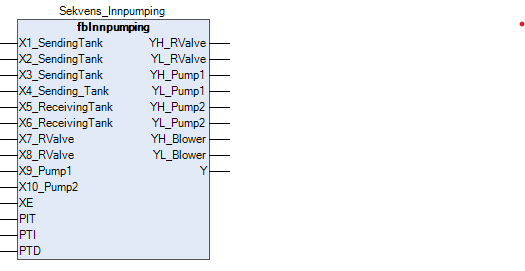
\includegraphics[width=1\textwidth]{Bilder/fbInnpumping.png}
        \caption{Innpumping}\label{fig:fbInnpumping}
    \end{subfigure}
    \hfill
    \begin{subfigure}[b]{0.3\textwidth}
        \centering
        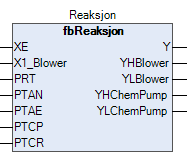
\includegraphics[width=1\textwidth]{Bilder/fbReaksjon.png}
        \caption{Reaksjon}\label{fig:fbReaksjon}
    \end{subfigure}
    \caption{Utklipp av tilstandslogikk}\label{fig:ReaksjonsFasen}
\end{figure}




	\newpage
\section{Oppbygging av programmet}
\thispagestyle{fancy}

\subsection{Programmeringsmetode}
For å sette saman alle funksjonsblokkene vi hadde programmert i \gls{ST}, valde vi å nytte \gls{Codesys} ``Continuous Function Chart'' (\gls{CFC}).
\gls{CFC} er eit grafisk programmeringsspråk som nyttar symbol og koplingar for å gjere programmet meir visuelt.

Alle samankoplingar av blokker valde vi å gjere i \gls{CFC}. Ved å nytte ein grafisk metode sikra vi oss god lesbarheit og
visuell forståelse av programmet. 

Alle inngangar og utgangar er leselege og enkle og forstå. \gls{CFC} i lag med god dokumentasjon vil kunne gi personar utan programmeringsbakgrunn
god forståelse av korleis programmet er oppbygd, utan å måtte lese kodelinjer.
\gls{CFC} gir eit godt grunnlag for feilsøking og analyse, dette bygger vidare på filosofien med eit enkelt og fleksibelt program.

Dersom antall koplingar og linjer gjorde programmet vanskeleg å lese var det også
mogleg å opprette ``source'' og ``links'' som oppretta ein trådlaus forbindelse gjennom ein unik ID.

\begin{figure}[htbp]
    \centering
    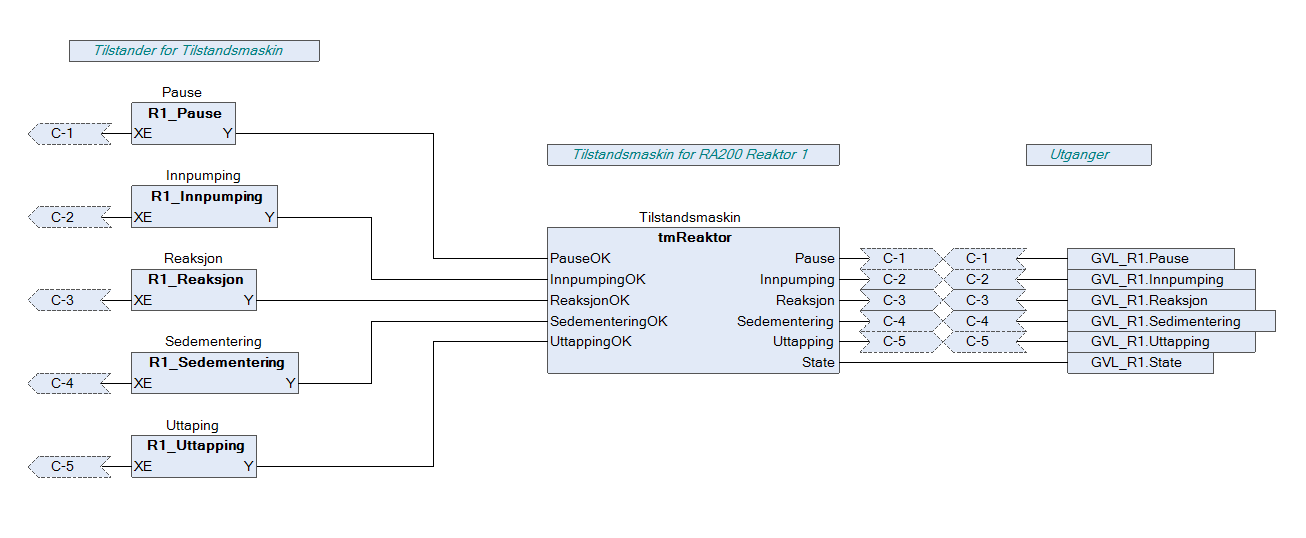
\includegraphics[width=1\textwidth]{Bilder/ReaktorPRG.png}
    \caption{Eksempel \gls{CFC} - Styring reaktor 1}\label{fig:CFCReaktor}
\end{figure}

\newpage

\subsection{Hovuddel}

Programmet er delt opp i tre hovuddelar, ei tilstandsmaskin for kvar reaktor og ein del for samling av felles reaktorfunksjonar.
Alle delane blir utført kvar \gls{PLS} syklus. 
Tilstandsmaskina har det overordna ansvaret og passar på kva tilstandslogikkblokk som nyttast.

Fellesfunksjonar er ei samling av funksjonsblokker og utrekningar som er felles for reaktorane, og er uavhengig av tilstandsmaskinene.
Driftsovervaking er ein sentral del av fellesfunksjonar, der gangtider og mengde prosessert vatn er døme utførte berekningar.

I nokre tilfelle, som ved rullering av sivbed, var vi avhengig at begge tilstandsmaskinene hadde same informasjon.
Dette løyste vi ved å lage ei funksjonsblokk ``fbSivbedRotation'', i felles funksjonar, som hentar inn og behandlar antall slamuttak for å rotere sivbed når ei gitt grense er nådd.
Denne informasjonen blir deretter sendt til kvar tilstandsmaskin som sørger for at begge reaktorane har same aktive sivbed.

\begin{figure}[htbp]
    \centering
    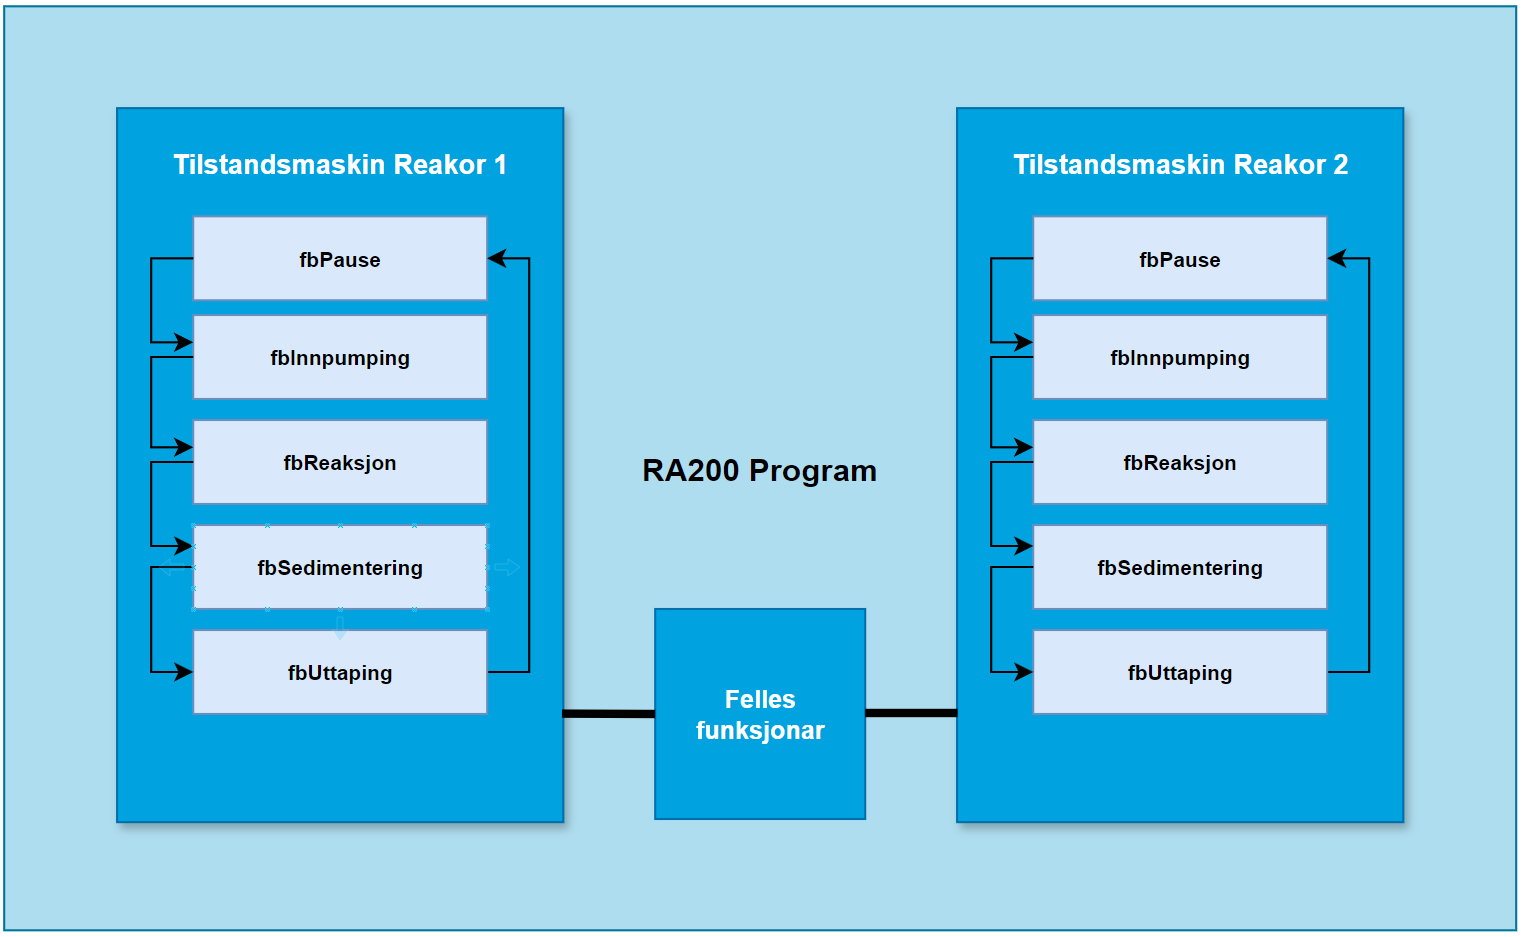
\includegraphics[width=1\textwidth]{Figurar/Oppbygging_Program.png}
    \caption{Illustrasjon oppbygging program}\label{fig:OppbyggingProgram}
\end{figure}

\newpage

\subsection{Styring tilstandslogikk}

Som tidlegare skildra er det tilstandslogikken som samarbeider med \gls{IEC} blokkene. Dette samarbeidet valde vi også å gjere i eit
\gls{CFC} vindu som gjorde kall og koplingar meir visuelt. \gls{CFC} vindauget fikk namn etter kva sekvens i \gls{SBR}-prosessen
den hadde ansvar for å styre. 

Oppbygginga av desse sekvensstyringane er gjort med inngangsblokker (\gls{MA} og \gls{MB}) øvst og utgangsblokker (\gls{SBE} og \gls{SBV}) i botn.
Mellom desse kjem tilstandslogikkblokka som inneheld styringslogikk.

\begin{figure}[htbp]
    \centering
    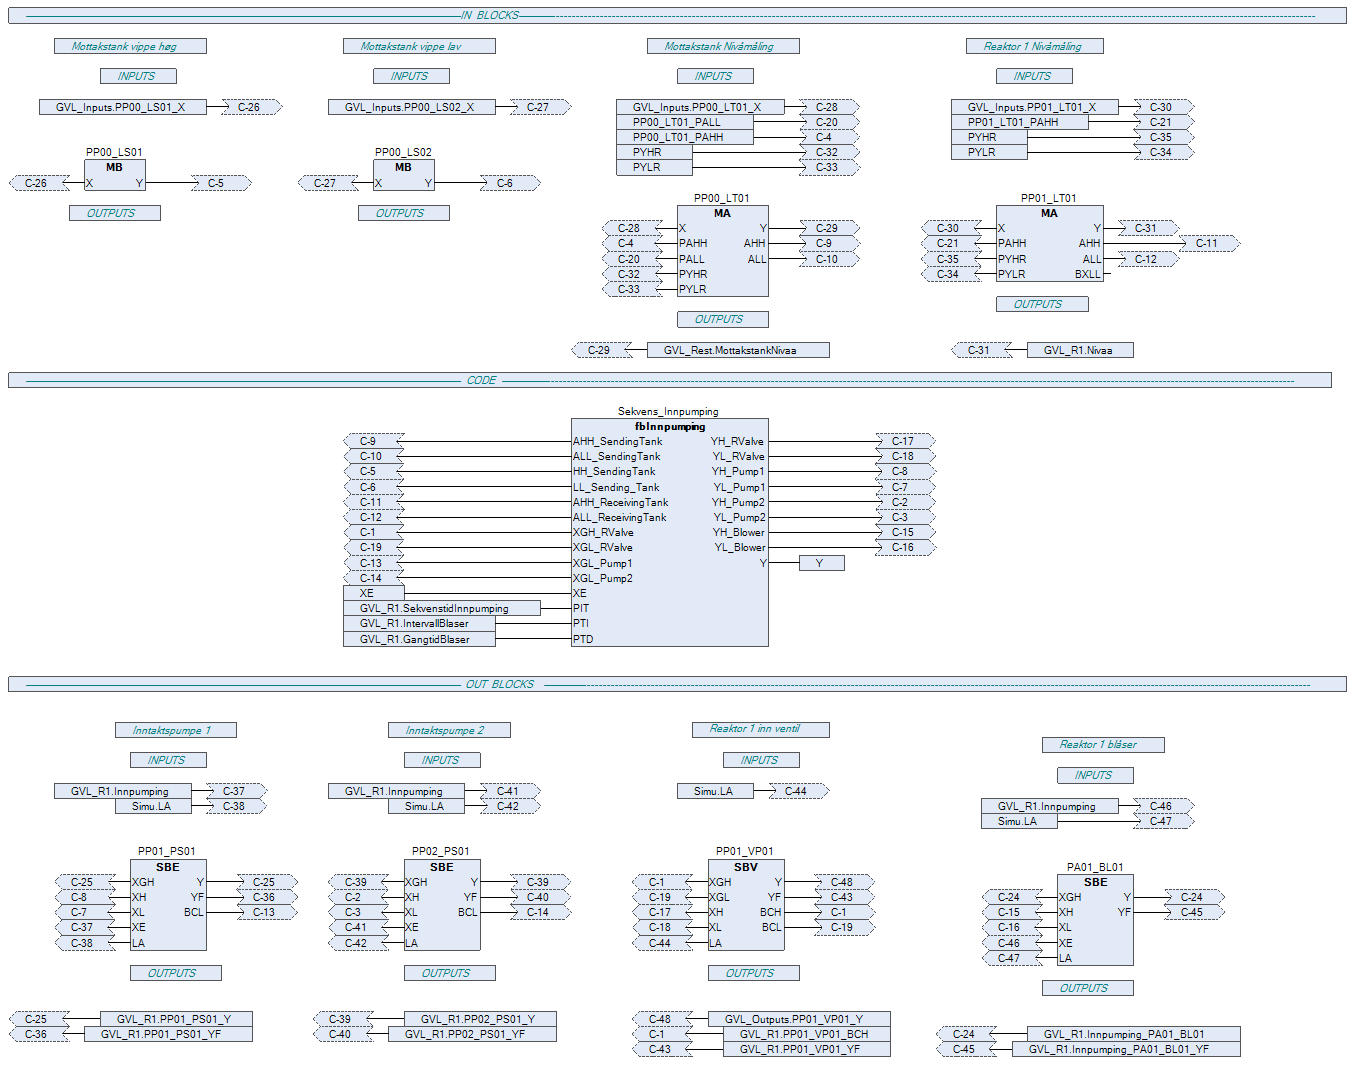
\includegraphics[width=1\textwidth]{Bilder/Heile_innpump.png}
    \caption{Eksempel \gls{CFC} - styring innpumping}\label{fig:CFCInnpumping}
\end{figure}

I denne figuren er ekstra inngangar, parameterinngangar og utgangar fjerna for å betre kunne visualisere koplingane og samarbeidet mellom
\gls{IEC} blokkene og tilstandslogikk.

\newpage


	\newpage
\section{Alarm og feilhandtering}
\thispagestyle{fancy}

% Skriver litt om introduksjon om alarm og feilhandtering
Alarm og feilhandtering utgjer ein sentral del av eit velfungerande styresystem. Det er avgjerande
at anlegget effektivt handterer og varslar om uønskte hendingar, slik at 
driftspersonalet blir varsla og nødvendige tiltak kan raskt setjast i verk.


% Skrive litt om codesys alarmhantering
For å varsle om alarm og feil i vårt program, har vi nytta oss av \gls{Codesys} sine
innebygde alarmhandteringsfunksjonar \citep{CodesysAlarm}. Desse funksjonane gir oss høve til å 
kontrollere, gruppere og prioritere alarmar, samt å sende informative tekstar til driftspersonalet.

% Skriver om alarmar både gamle og nye.
\gls{IEC}-blokkene som vi har utvikla, gir oss moglegheita til å detektere ulike typar hendingar
som feil, alarmar og forvarsel.
Dei forkjellige blokkene har ein variert mengde med feil som skal kunne detekterast og varslast.
Forløpet er slik at feil blir detektert og ein boolsk variabel \gls{YF} blir sett til sann, 
samt at ein heiltalsverdi \gls{YFI} indikerar kva type feil som har inntruffe.\newline
Alle desse moglege typane varslingar, som er omtala i vedlegg E, 
er samla i programmet vårt saman 
med dei aktive varslingane som er i bruk på Sande reinseanlegg i dag.

Vi har valgt å dele opp alle varslingane i fire forskjellige grupper:

\begin{itemize}
    \item \textbf{Feil}          (Der systemet ikkje fungerar, t.d. sensorfeil og blokkfeil)
    \item \textbf{Alarmar}       (Kritiske prosessparameterar, t.d straumbrudd og veldig høge nivå)
    \item \textbf{Forvarsel}     (prosessparameterar som nærmar seg kritisk nivå)
    \item \textbf{Informasjon}   (Prosessinformasjon med nytteverdi)
\end{itemize}

Ved å kategorisere varslingar i fire ulike grupper med forskjellige prioriteringsnivå,
vil systemet og driftspersonalet enklare kunne forstå samanhengen og alvoret i varslingane. \newline
Korleis dei ulike alarmane blir definert og prioriterte må evaluerast i samråd med \gls{Sunnfjord Kommune}.

\newpage

	\section{Utfordringar}
\thispagestyle{fancy}

\subsection{Utgangsblokker med signalkonflikt}
Nokre komponentar skulle nyttast i fleire tilstandar og vi opplevde 
utfordringar med å ha fleire utgangsblokker for ein komponent.
Orginalt var dette løyst med fleire kall av ei utgangsblokk i forskjellige \gls{CFC} vindauge.
Kalla av dei ulike blokkene skreiv forskjellige signal til komponenten, og
sendte høg signal blei kontinuerleg overskreve.

Vi møtte denne utfordringa fleire plassar, t.d. i pumpestyringa,
der kvar reaktor skulle kunne styre den same pumpa.
Dette løyste vi ved å nytte ein unik utgangsvariabel for kvar blokk, 
og deretter skrive til ei blokk som samla signala til komponenten og satt utgangen til riktig verdi.

\subsection{Mangel på sensorikk}

Anlegget har begrensa mengde sensorikk. 
Dette har ført til at vi må berekne, estimere og programmere rundt denne mangelen.

Som døme har anlegget ein funksjon for å aktivere
høgbelastningsmodus ved høg tilstrøyming, 
men anlegget har ingen form for strøymningsmålar.\newline
Grunna dette har vi vore nøydd til å kalkulere ein teoretisk tilstrøyming basert på endringa av volumet i mottakstanken.

Sjølv om slike løysningar kan fungere, er det ikkje optimalt for anleggets drift.
Estimering av prosessverdiar vil redusere nøyaktigheit i styresystemet og
unødvendig prosessorkraft vil bli nytta på berekningar som enkelt kunne vore erstatta av ein sensor.\newline
Det det også krevd ekstra tid å programmere desse funksjonane.




	% Kapittel 9 Dokumentasjon
	\chapter{Dokumentasjon}
\thispagestyle{fancy}

I dette kapittelet tar vi for oss og samlar dokumentasjonen av programmet som er utarbeidd.
	\section{Dokumentasjon av funksjonsblokker}
\thispagestyle{fancy}

Alle funskjonar og blokker som er utarbeida i programmet har eit eigen dokumentasjonsdokument. \newline
I dokumentet er bruk, funksjonalitet, inngangar, utgangar og parameterer er beskreve i djupare detalje.
Dokumentet inneheld versjonshistorikk som oppdatterast ved aktuelle endringar, liste over omgrep og forkortingar samt
ei liste på aktuelle programmeringsbiblioteker som trengs for å ta blokka i bruk.
Dokumentet er utvikla etter ein eigen mal og er standarisert for alle blokkene som er brukt i programmet.

Dokumentasjon til alle funksjonar og funksjonsblokker er tilgjengeleg via appendix (Appendix xXx)
	\section{Forrigling}
\thispagestyle{fancy}

For å unngå utilsikta situasjonar har vi implementert forriglingar.
Desse forriglingane er inkludert i tilstandslogikkblokkene.\newline
\gls{IEC} blokkene tilbyr også funksjonalitet som gjer det mogleg å handheve forriglingar mellom komponentar.

Det ligg forrigling på styring av matepumpene til reaktorane. Det skal ikkje være mogleg at begge pumpene går samtidig
og beskyttelse for dette er handtert i funksjonsblokka ``fbSwap''(\ref{sec:1}).

Det skal heller ikkje førekomme at begge reaktorane er i tilstand innpumping samstundes.
Sidan tilstandsmaskinene som styrer kvar reaktor er uavhengige av kvarandre, måtte vi løyse dette med ein
\gls{Globalvariabel}. Denne variabelen blokkerer overgangen frå pause til innpumping dersom ein reaktor allereie er i innpumping.

Programmet har overordna kontroll med at tilstandsmaskinene gir signal til XE, 
slik at komponentane som ikkje er i bruk ikkje er tilgjengeleg.

\newpage







	\section{Tilstandsovergangsbetingelsar}
\thispagestyle{fancy}

For at tilstandsmaskina skal få lov til å endre tilstand, må nokre spesefikke betingelsar vere oppfylt.
Fleire av betingelsane er tidsstyrte, og alle desse tidene er justerbare via parameter.\newline
For å kunne gi ei klarare framstilling av logikken har vi valt å presentere betingelsane grafisk.
Vi har utarbeidd eit skjema som dokumenterer alle overgangsbetingelsane i tilstandsmaskina.\newline \newline

\begin{figure}[htbp]
    \centering
    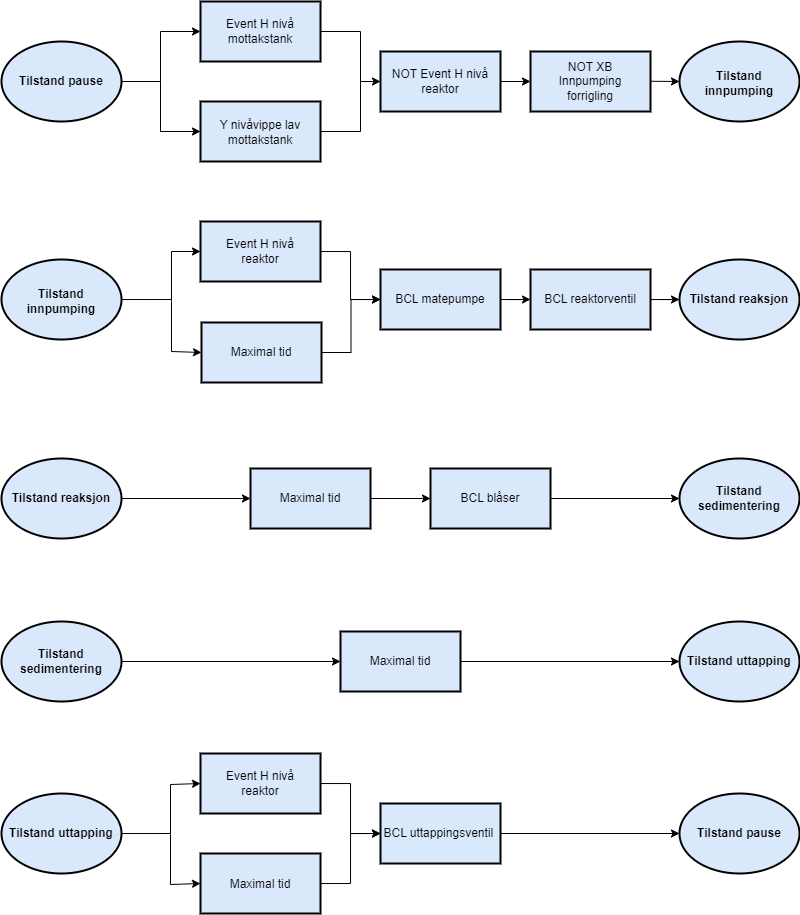
\includegraphics[scale=0.5]{Figurar/Tilstandsovergang.drawio.png}
    \caption{Grafisk presentasjon av overgangsbetingelsar}\label{fig:Tilstandsovergangsbetingelsar}
\end{figure}

\newpage		
	\section{IO-liste}
\thispagestyle{fancy}

Når det gjeld \gls{IO}-liste, har vi tatt utgangspunkt i den eksisterande IO frå styresystemet på Sande.\newline Sida vår løysning baserar seg på ei teoretisk løysing,
har vi nytta dei eksisterande sensorane i programmet vårt. Vi har ikkje konstruert løysinga mot ein eksisterande \gls{PLS}, sidan vi 
ikkje har ein fysisk \gls{PLS} å planleggje  mot. \gls{IO}-liste er lagt ved som (vedlegg J)

%Når det gjelder \gls{IO} liste, så har vi ikkje noko konkret å visa til, enn den gamle lista sidan våra løysningsforslag baserer seg på ein teoretisk løysning.
%Vi har difor tatt utgangspunkt i ein minimum I/O som allereie ligger til stades i frå det tidlegare anlegget (Vedlegg J) 
%(Vi har den gamle IO, men den nye er ikkje konstruet da vi ikkje har ein fysisk pls å planlegge mot.)

%\includepdf[pages=1, scale=1, pagecommand={\thispagestyle{empty}}]{Appendix/IOliste.pdf}
%\includepdf[pages=2, scale=1, pagecommand={\thispagestyle{empty}}]{Appendix/IOliste.pdf}



%I tillegg så har vi laget til moglegheit for fleire inngangar basert på ønsket tilleggsmål gitt av arbeidsgivar. 
%Dette er tilrettelagt for til dømes tilbakemelding av ventilar, flowmåler og temperaturgivera.
%Dette er funksjonalitet som er veldig enkle å legge til i ettertid, da programmet er bygget opp med dette i tankane.


	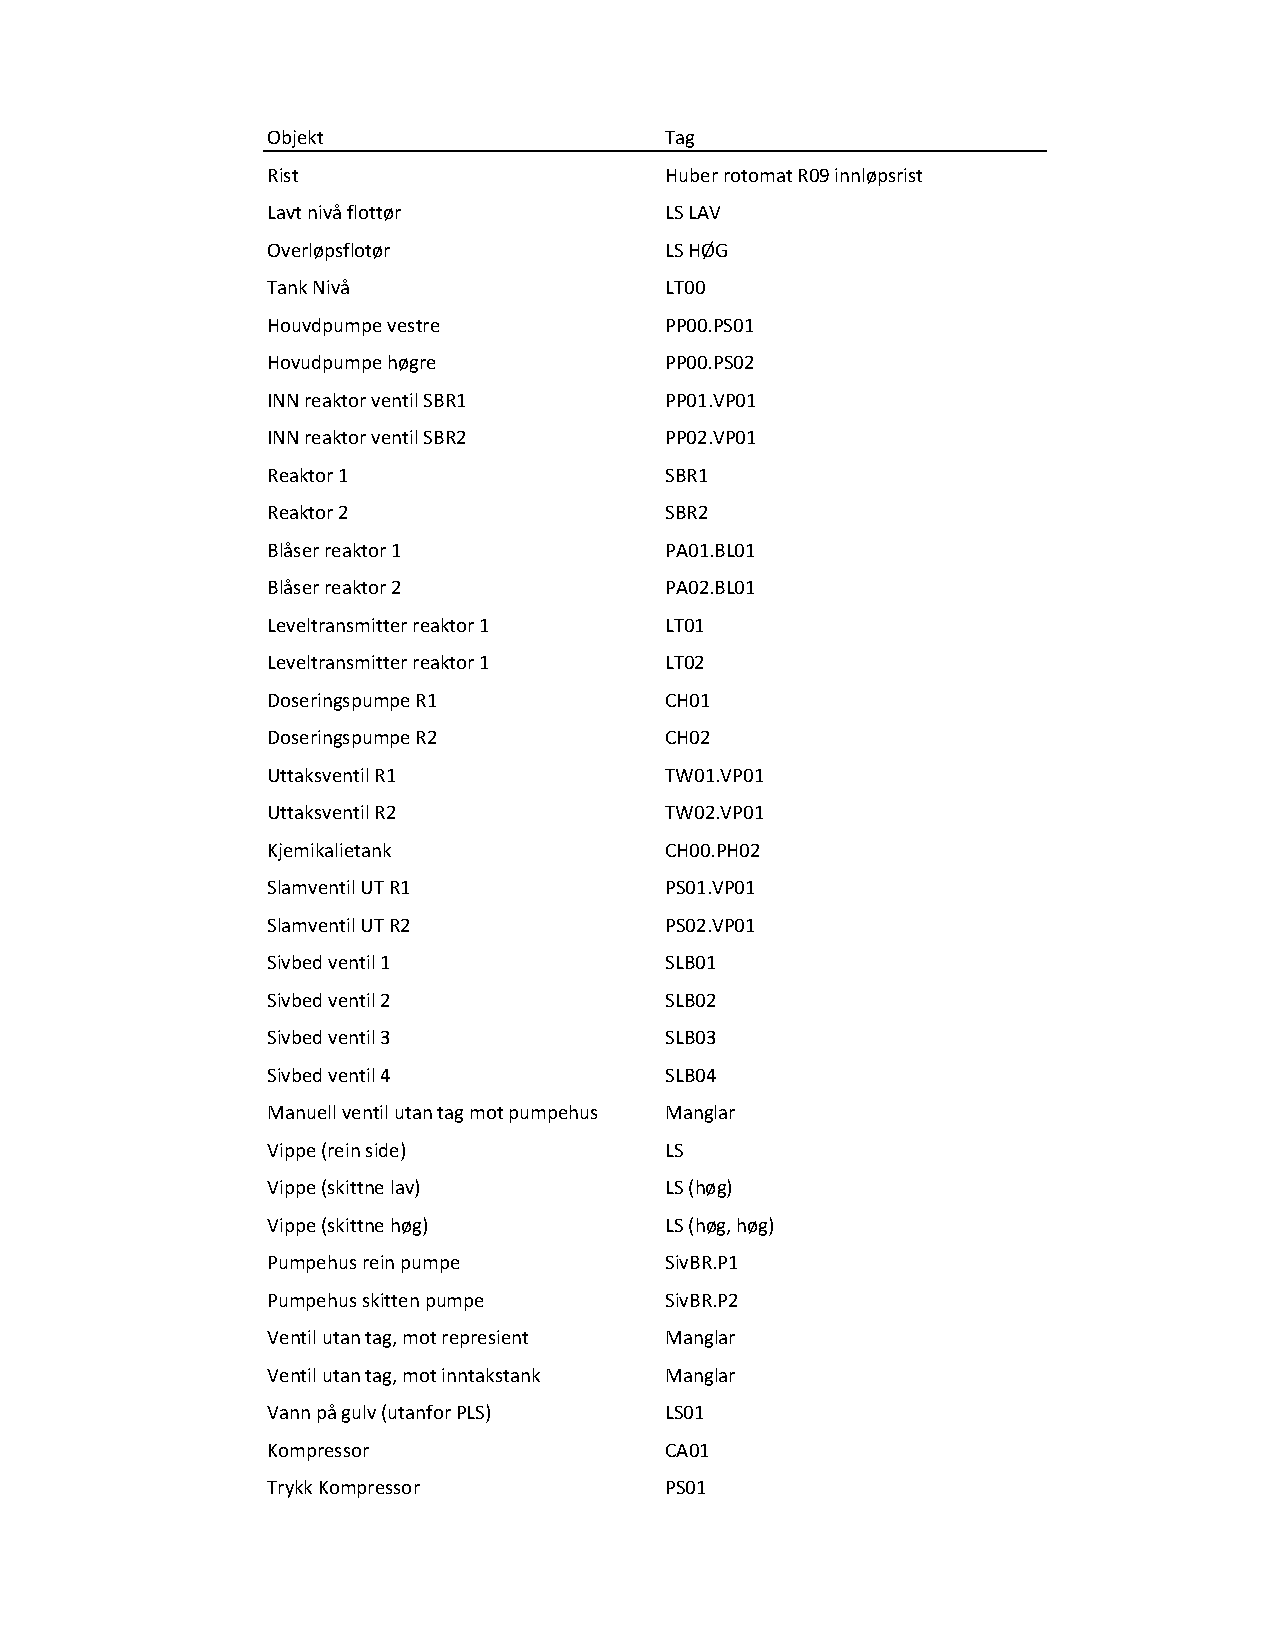
\includepdf[pages=1, scale=0.75, pagecommand={\section{Objektliste}\thispagestyle{empty}}]{Appendix/Objektliste_midlertidig.pdf}

\newpage

	\newpage
\section{SCD}
\thispagestyle{fancy}

\gls{SCD} utgjer grunnlaget for det meste av programmeringsdokumentasjonen i oppgåva.
Diagrammet er delt opp sidevegs og sekvensvis og viser styring mellom program og komponentar i kvar enkelt sekvens,
samt ei side for resterande felles styring.

Prosessen i \gls{SCD}en (blå linjer) er basert på \gls{PID} som blei laga etter gjennomgangen av anlegget i kapittel \ref{sec:6}.
\gls{SCD} tar omsyn til programmerbart utstyr og har derfor ikkje med manuelle ventilar, tilbakeslagsventilar eller liknande.

For å representere eigne funksjonsblokker var vi nøydd å legge dei inn i \gls{SCD}en.
\gls{SCD} verktøyet hadde moglegheit for å legge til eigendefinerte blokker med respektive inngangar og utgangar.

Funksjonsblokker og \gls{IEC} funksjonstemplata nytta i \gls{SCD} er dei same som vi har laga og brukt i programmeringsdelen. 
Dei stipla linjene viser koplingar mellom blokker og komponentar. \newline
I enkelte diagram førte antal linjer til at diagrammet vart vanskeleg å lese. 
Vi har derfor nytta koplingar med unik ID, liknande som i CFC vindauget.

Tilstanslogikkblokker har fått eigne forkortingar i \gls{SCD}en.
Dette er dei relevante forkortingane for å forstå blokkene og diagrammet.

\begin{itemize}
    \item \textbf{SM}:   Tilstandsmaskin
    \item \textbf{FBP}:  Funksjonsblokk pause
    \item \textbf{FBI}:  Funksjonsblokk innpumping
    \item \textbf{FBR}:  Funksjonsblokk reaksjon
    \item \textbf{FBS}:  Funksjonsblokk sedimentering
    \item \textbf{FBU}:  Funksjonsblokk uttapping
    \item \textbf{FBPH}: Funksjonsblokk pumpehus
\end{itemize}

Heile \gls{SCD} er tilgjengelig i vedlegg. (Vedlegg H). \newline
\newpage

\begin{tikzpicture}[remember picture, overlay]
    % Include the PDF page rotated, positioned at the center of the page
    \node[inner sep=0pt] at (current page.center) {
        \includegraphics[page=2,angle=90, scale=1, keepaspectratio]{Bilder/SCD.pdf}
    };

    % Place the caption at the bottom of the page
    \node[anchor=south, yshift=10mm] at (current page.south) { % Adjust yshift to position the caption
        \begin{minipage}{\textwidth}
            \centering
            \captionof{figure}{SCD av innpumpingssekvens}
            \label{fig:SCD}
        \end{minipage}
    };
\end{tikzpicture}


	% Kapittel 10 Simulering og verifisering
	\chapter{Simulering og verifisering}
\thispagestyle{fancy}

Simulering er ein sentral del når ein utviklar eit nytt styresystem
og gir oss moglegheiten å validere at at programmet møter designspesifkasjon og har ønska effekt.
Testing og simulering vil redusere risiko, forbetre kvalitet og auke pålitlegheit.

-Stikkord vegard
- Mange parametera må vere riktig

	\section{Kontinuerlig simulering}
\thispagestyle{fancy}

Undervegs i programmeringa har vi utført kontinuerlege testar og simuleringar av blokkene vi har utvikla, noko
som har våre ein viktig del av arbeidsmetodane vi har brukt i oppgåva. 

Kontinuerleg simulering er små testar som blir utførte medan ein programmerar.
Det er ikkje ein isolert testfase med klare start- og stoppunkt, men heller små kontinuerlege testar og verifiseringar som gir oss ein indikasjon
på om arbeidet følgjer spesifikasjon.

I denne oppgåva nytta vi kontinuerleg simulering i programmeringsfasen av \gls{IEC} blokkene.
Desse blokkene hadde mange funksjonar som ikkje nødvendigvis var avhengige av kvarandre,
som gjorde det mogleg å gjennomføra små, enkle testar på dei ulike områda utan at heile blokka var ferdigstilt.\newline
Som eit døme, skal \gls{RX} resette ein utgang \gls{Y}. Dette blir implementert og deretter testa ved hjelp av simulering.
Kva som til slutt skal sette utgangen \gls{Y} høg er ikkje relevant i dette tilfellet. Vi har likevel implementert 
og testa at ein reset vil fungere.


\begin{figure}[htbp]
    \centering
    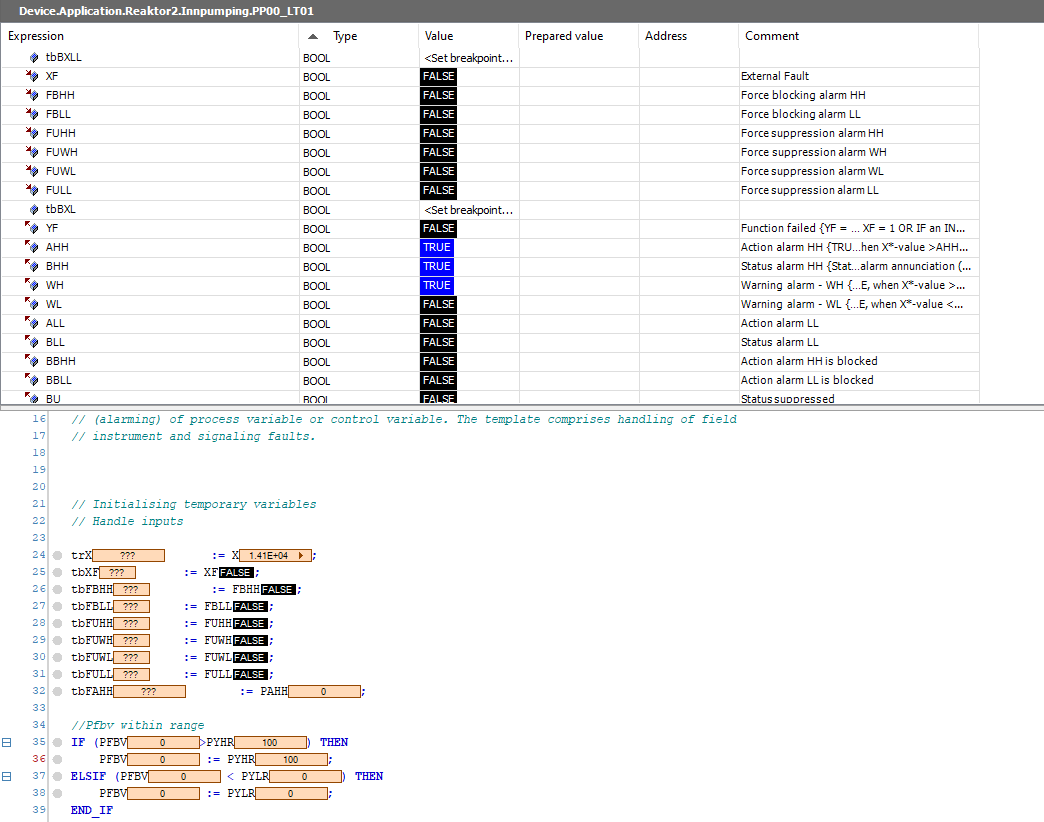
\includegraphics[width=0.8\textwidth]{Bilder/kontinuerligSimulering.png}
    \caption{Kontinuerleg testing ved manipulasjon av verdiar}\label{fig:KontinuerlegSimulering}
\end{figure}


\newpage

	\section{Simuleringsblokker}
\thispagestyle{fancy}

For å skape eit realistisk miljø for testing, lagde vi nokre simuleringsblokker.
Desse blokkene etterliknar driftssituasjonar og gjer simulering enklare og meir effektivt.
Vi lagde hovudsakleg to slike blokker, ei simulerer fylling av tank
og ei for tilbakemelding frå ventilar.

Blokk for tanksimulering er enkel og programmert spesifikt reinseanlegget, 
som har ein mottakstank og to reaktorar.
Det er lite truleg at desse simuleringsblokkene vil bli nytta vidare, men dei gav
oss den realismen vi trengte.

Desse blokkene forenkla også sjølve arbeidet med simuleringa.
Før vi utvikla blokka for tilbakemelding på ventilar, 
gav vi manuelt kvar ventil XGH eller XGL basert på den tiltenkte stillinga (open/stengd). \newline
Dette fungerer greitt dersom ein testar ei ventilblokk, men
når simuleringa omfattar større delar av programmet blir denne jobben tidkrevjande.

På desse blokkene har vi tatt oss meir friheit i namngiving og feilhandtering, sidan blokkene ikkje skal nyttast når programmet er ferdigstilt.


\begin{figure}[htbp]
    \centering
    \begin{subfigure}[b]{0.3\textwidth}
        \centering
        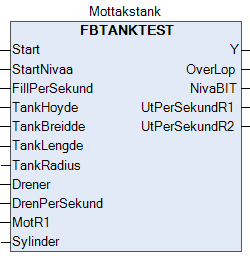
\includegraphics[width=0.9\textwidth]{Figurar/TankSim.png}
        \caption{Tank}\label{fig:TankSim}
    \end{subfigure}
    \hfill
    \begin{subfigure}[b]{0.3\textwidth}
        \centering
        \includegraphics[width=0.9\textwidth]{Figurar/ValveSim.png}
        \caption{Ventil}\label{fig:ValveSim}
    \end{subfigure}
    \caption{Simuleringsblokker}\label{fig:SimuleringsBlokker}
\end{figure}

\newpage
	\section{Simuleringsvindu}
\thispagestyle{fancy}

Når ein tester og simulerer eit prosjekt kan det bli mange variablar og komponentar
og halde styr på. Derfor er det viktig at ein sorterer og behalder den informasjonen ein
ønsker og klarer å representere denne på ein god måte.

Codesys Visualization er eit grafisk verktøy der ein kan representere informasjon
ved hjelp av grafiske elementer. Dette gav oss mulighet til presentere tankar, ventilar og pumper
ved hjelp av bilder og lys. 
Dette gjorde det mykje lettare for oss og oppdage eventuelle feil eller fastslå at ting fungerte.

Vi brukte visualiseringsverktøyet til å lage eit fullskala simuleringsvindu der kvar komponent
var knytt til sitt spesefikke grafiske symbol. Dette vinduet brukte vi ilag med simuleringa
av programmet og knytta dei relevante inngangssignala mot knapper. 
Dette gjorde at vi til slutt hadde eit grensesnitt mot programmet og enkelt kunne simulere
forskjellige driftssitasjonar og enkelt konkludere med resultat.

Simuleringsvinduet er ikkje tiltenkt å være noko 
HMI og tar ikkje hensys til aktuelle normer og krav

\begin{figure}[htbp]
    \centering
    \includegraphics[width=0.8\textwidth]{Bilder/Codesys symbol.png}
    \caption{Eksempel Codesys visualisering}\label{fig:reaktorsoner}
\end{figure}

\newpage

	\section{Fullskala simulering}
\subsection{Oppsett}
Med simuleringsblokkene klare og eit simuleringsvindauge til å vise resultata, var vi
no klare til å starte simuleringa av reinseanlegget.
Vi implementerte ventil-simuleringsblokka på alle ventilane i programmet og oppretta eit
nytt \gls{CFC} vindauge som kopla tanksimuleringa av mottakstanken og reaktorane i saman med resten av
programmet. Vi valde å starte med fleire små simuleringar før vi gjekk over til å simulere heile reinseanlegget med full funksjonalitet.

Simuleringa er satt opp slik at tilstrøyminga til anlegget kan justerast av ein glidebrytar.
Dersom ein av reaktorane er i innpumpingssekvens, simulerer vi flytting av avlaupsvatn
basert på pumpekurver og løftehøgder.

Reaktortilstand er presentert med ein tekstvariabel, og
dei aktuelle tidsparameterane, som t.d. tid for reaksjonssekvensar,
er reduserte for å akselerere simuleringa.

Vi har også laga ein alarmlogg for alle moglege alarmar anlegget kan generere, 
uavhengig om dei er relevante for sluttprogrammet eller ikkje.
Dette gir oss ein verdifull innsikt i eventuelle feil som kan oppstå og korleis programmet fungera i sin heilheit.

\thispagestyle{fancy}
\begin{figure}[htbp]
    \centering
    \includegraphics[scale=0.45]{Bilder/Simuleringsbilde.png}
    \caption{Oppsett av simuleringsvindauge}\label{fig:Simulering}
\end{figure}

\newpage

\subsection{Resultat}

Som forventa dukka det opp avvik og ``bugs'' når vi starta med simuleringa.
Nokre av desse var av mindre betydning og blei utbetra undervegs i prosessen, som t.d. den tiltenkte
reaktorforriglinga som ikkje fungerte på overgangen frå pause til innpumpingssekvens. \newline
Andre avvik krevde meir inngåande arbeid og tilbakevending til programmeringa, der problema som oftast låg i skrivefeil, gløymde logiske operasjonar,
\gls{CFC} koplingar som var plassert feil eller konfigurasjonsfeil.

Simuleringa av programmet var svært vellykka og vi fekk samla masse verdifull informasjon frå anlegget i simulert drift. 
Den visuelle representasjonen var oversiktleg, der ein kunne sjå programmet i drift, og det var enkelt å sjå kva programmet gjorde og oppdage feil. 

Vi verifiserte at programmet i hovudsak fungerer som planlagt og vi er no klare til å gjennomføre ei større simulering,
der vi implementerer dei resterande funksjonsblokkene og siktar mot ein fullskala test.







	% Kapittel 11 Diskusjon
	\chapter{Diskusjon}
\thispagestyle{fancy}
DISKUTERE
I slutten av april avslutta vi programeringsfasen våra, og starta rapportfasen.

KRAV OG MÅLOPPNÅING
DELMÅL

1. fsd 
2. Programmering (Skriv at vi kunne sikkert ha brukt meir av IEC blokk funksjonane)
3. Verifisering og simuering.

Tillegsmål!
Skrive om HMI og mangelen på denne er fordi oppdragsgivar ikkje har noko plan for korleis
dei skal løyse HMI-planen for anlegget. 

	\section{Vegen videre for anlegget}
\thispagestyle{fancy}

\subsection{Ombygging}

Dersom den teoretiske bacheloroppgåva vår skal realiserast i praksis trenger anlegget fysiske oppgraderingar.
Reinseanlegget idag tilfredsstiller ikkje fleire relevante lover og forskrifter rundt industri og offentleg infrastruktur.
Mykje av denne delen er utanfor vårt fokusområde men reinseanlegget har foreksempel ingen handtering eller moglegheitar for naudstopp.
Vi anser det som viktig at koden og programmet ikkje settast i drift dersom anlegget ikkje gjennomgår ein grundig sikkerheitsanalyse.
Vi forventer då ein større ombygging i eit slikt tilfelle der fleire aspekter av anlegget kan oppgraderast

\newpage

\subsection{Anbefalingar sensorikk}

For å betre anlegget og styresystemet ytterlegare vil det være nyttig å få inn meir instrumentering. 
Auka sensorikk vil forbetre styresystemet ved å samle meir og nøyaktig data om tilstanden og ytelsen til systemet. 
Med meir data vil styresystemet bli meir automatisk og vil kunne tilpassast varierande forhold meir effektivt. 
Systemet vil og ha moglegheita til å oppdage avvik og agere tidlegare utan manuelle inngrep, noko som igjen aukar automasjonsevna.

Basert på vår nyerfarte kunnskap av annlegget og styresystemet presenterer vi ein
anbefaling på oppgradering av instrumentering som ville forbetre reinseanlegget. 
Sjølv om all sensorikk vil være verdifull, har vi vurdert kost-nytte og anbefaler kun sensorikk som vil gi tilstrekkeleg verdi.

\begin{itemize}
    \item \textbf{Strøymingsmålar} \newline
        Strøymingmålar i anlegget vil gi nøyaktige tall på mengder vatn som er i anlegget.
        Dette vil gi bedre kontroll på aktivering av høgbelastningsmodus og kontroll og rapportering av driftsdata.
        Fleire strøymningsmålarar er moglege men minimumsanbefaling er vatn inn og ut av anlegget.
    \item \textbf{Energimåling} \newline
        Måling av energi vil gi moglegeit å analyse energiforbruket for å redusere kostnadar og effektivisere prosessar.
        Komponentspesefikk energimåling kan også brukast til overvåking av utstyr for å oppdage slitasje og feil.
    \item \textbf{Reaktormålingar} \newline
        Oksygen, PH og temperatur er alle kritiske verdiar for å oppnå god biologisk reinsing i reaktorane. \newline
        Ved å ha kontroll på desse parameterane vil reaktoren kunne finjusterast for å effektivitere den biologiske reinseprosessen.
    \item \textbf{Tilbakemeldingar} \newline
        Anlegget har begrensa tilbakemeldingar på utstyr, spesielt ingen innan ventilstyring.
        Tilbakemelding er essensielt for prosesstyring, feiloppdagelse og sikkerheit.
        Utan tilbakemeldingar er reinseanlegget meir sårbar for feil som ikkje blir oppdaga før det er for seint 
        og slike situasjonar vil kunne resultere i nedetid, overlaup og andre utilsikta hendelser.
    \item \textbf{Forbetra nivåmåling} \newline
        Ei forbetring av dei akutelle nivåmålingane i anlegget vil gi meir nøyaktige mål på slammengde og slamnivå i reaktorane.
        Det vil då være mogleg å finne det eksakte skilljet mellom slam og reinsa vatn etter ein sedimenteringssekvens som igjen
        gir bedre oversikt over tilstanden til den biologiske reinseprosessen.
    \item \textbf{Oppløysning} \newline
        Oppløysning på analoge målingar er idag kunn 0-1000 bit på 4-20mA.(Sjå datablad appendix xXx) \newline
        Oppgradering av måleoppløysning vil gjere kvar eksisterande og nye analoge målingar
        meir nøyaktig som igjen gir moglegheit for betre styring og regulering.
\end{itemize}
\newpage


	\section{Vegen vidare for programmet}
\thispagestyle{fancy}

Programmeringsarbeidet hadde eit så stort omfang at vi ikkje klarte å ferdigstille programmet.
Etter å ha innsett at vi ikkje ville nå målet, måtte vi gjere nokre val angåande prioriteringa av ressursane våre. 
Vi valde å fokusere på å gjennomføre ei god samla simulering av programmet i staden for å arbeide vidare med ferdigstilling av funksjonar.

\subsection{Programmering}

Vegen vidare for programmet er først og fremst ferdigstilling av funksjonane som ikkje er komplette, og 
implementering av funksjonar som er laga til men ikkje tatt i bruk. 
Det står også at arbeid på feilhandtering og korleis anlegget skal agere på spesifikke feilsituasjonar.

Følgande kjem punkter vi ynskjer å arbeide vidare med.

\begin{itemize}
    \item Styring av pumpehuset er forberedt men ikkje programmert. 
    \item Ferdigstilling av høgbelastningsmodus.
    \item Generell feilhandtering
    \item Automatisk prøvetaking er ikkje blitt programmert.
    %\item Implementere beskyttelse av parametere.
\end{itemize}


% Begge desse er vel forsåvidt berre MB blokker inn, så må det skje ting i spesefikk feilhantering istaden
%\item Sensor for vann på golv er ikkje programmert.
%\item Tilbakemelding frå pressostat på kompressor er ikkje programmert.

\subsection{Simulering}

Det står framleis at mykje simulering og testing av programmet før ein kan anse det som ferdig verifisert.
Til dømes er funksjonsblokkene for slamuttapping og sivebedrotasjon testa separat, men ikkje simulert i sin heilskap saman med
tilstandsmaskinene og resterande program.

Under testing av eit slikt program som dette bør ein aktivt leite og prøve å identifisere feil og manglar for å gjere programmet best mogleg.
For blokkparameterer manglar eksempelvis fleire beskyttelsar mot ulovlege parameterverdiar, noko som vil bli oppdaga gjennom meir omfattande simulering.

Ved å investere meir tid i vidare simuleringsfase sikrar vi at programmet oppfyller forventningane til \gls{Sunnfjord Kommune} og at ein eventuell
praktisk innkøyringsfase går effektivt. \newline
Programmet er no satt opp i simuleringsmodus, og det må tilbakestillast til original tilstand før det kan brukast. 
Simuleringsmodus har endra fleire parameterverdiar og er kopla opp i mot simuleringsblokker.  



\newpage
	\section{Måloppnåing}
\thispagestyle{fancy}

\newpage
	\section{Lærdom og forbetringspotensial}
\thispagestyle{fancy}

Oppgåva har bydd på eit bratt lærekurve og når vi ser tilbake på arbeidet som er utført
ser vi fleire moglegheitar for forbetring.

Etter læring og dokumenteringa av anlegget var vi ivrige på å byrje med kodinga.
Vi valgte å starte fortløpade og så lære litt undervegs.
Dette gjorde at vi på fleire plasser var nødt til å ta ting oppigjen grunna at vi hadde missforstått standarar og enkelte gangar missforstått kvarande.
I etterklokspaenslys skulle vi gjerne ha lest litt meir om IEC blokkene og tatt litt betre tid før vi byrja å programmere dei.

Vi kan også sjå i etterkant av programmeringa at vi kunne ha nytta funksjonalitetane til IEC blokkene betre.
Med ordentleg bruk av alle dei funksjonalitetane som vi programerte kunne ein kanskje ha redusert all tilstandslogikk
til eit par logiske setningar og kanskje fjerna den i sin heilheit.

Navngiving på inngangar, utgangar og parameter har også moglegheit for forbetring.
I starten var vi flinke og satt av den nødvendige tida for å få navn korrekt, men ettersom tida blei knappare utover i oppgåva
blei namngivinga dårlegare. Dette gjorde at vi var nøyd å ta alle desse namna igjen. \newline
Vi skulle også satt oss ned på forkant av programmering å blitt enige om kva språk kommentarar, navn og forklaringar skulle komme på.
Her var vi ikkje konsekvente på, og programmet endte opp med litt bokmål, litt nynorsk og ein del engelsk.

Vi ser også at vi gikk litt for detaljert i reinseanleggets virkemåte.
Sjølv om denne delen av oppgåva var vesentlig ser vi no at noko av arbeidet vi brukte tid på kanskje ikkje var naudvendig.


Igjennom denne bacheloroppgåva har vi henta inn mykje ny kunnskap og erfaring.
Oppgåva har gitt oss utfordringar og læringskurver vi før ikkje trudde var moglege.
Vi har blandt anna lært og utdjupa oss innan:

\begin{itemize}
    \item Offentleg infrastruktur
    \item Kunde kommunikasjon
    \item Programmering av større styresystemer i PLS
    \item Programmering av PLS i Codesys
    \item IEC 61131-3 og IEC PAS 63131
    \item Github intergrering
    \item Rapportskriving i Latex
\end{itemize}



	
	% Kapittel 12 Konklusjon
	\chapter{Konklusjon}
\thispagestyle{fancy}


Dette låg under diskusjon.
1. fsd 
2. Programmering (Skriv at vi kunne sikkert ha brukt meir av IEC blokk funksjonane)
3. Verifisering og simuering.

Tillegsmål!
Skrive om HMI og mangelen på denne er fordi oppdragsgivar ikkje har noko plan for korleis
dei skal løyse HMI-planen for anlegget. 


Må skrivast i fortid, Konklusjon vs Avslutting?

Fra chatgpt
Oppsummer hovedfunnene: Gjennomgå kort de viktigste funnene og resultatene av studien din.

Relater til problemstillingen: Diskuter hvordan funnene svarer på problemstillingen eller forskningsspørsmålene 
som ble presentert i innledningen.

Diskuter implikasjoner: Vurder hvilke implikasjoner dine funn kan ha for fagfeltet ditt eller relevante praksisområder. 
Hvordan kan resultatene påvirke fremtidig forskning eller handling?

Styrker og svakheter: Reflekter over styrker og begrensninger ved studien din. 
Hvilke faktorer kan ha påvirket resultatene,
----

sokogskriv.no - tips
Pek på nye problemstillinger som du har kommet over gjennom arbeidet
Ta fatt i ubesvarte spørsmål fra ditt eget prosjekt, og pek på mulig oppfølging og nye, potensielle prosjekter
Konklusjonen følger av det som er sagt
Oppgaven «biter seg selv i halen»

https://www.superprof.no/blog/bachelor-konklusjon/

	\cleardoublepage
	\pagestyle{fancy}
	\renewcommand{\glossaryname}{Ordliste} % Denne er med for å kunne endre navn på ordlista
	\thispagestyle{fancy} 
	\printglossaries %Printer ut alle ord som er brukt frå ordlista







	%Referanseliste (Berre for test, citep må flyttast inn i teksten)
	%\clearpage
	%\chapter{Referansar} % sjekk om det skal være slik, for å få den opp i innhaldslista.
	\clearpage
	
	\bibliography{Referansar} % Dette er ein referanse til Referansar.bib
	\addcontentsline{toc}{chapter}{Referansar}  % Adds the unnumbered chapter to the table of contents
	\thispagestyle{fancy} % Må vere her for å sette pages tyle
	

	% Create a partial table of contents for appendices
	% Generate the list of appendices
	% Start of appendices, capture contents for appendices list
	%\begin{appendices}
		% This command initializes the recording of contents for appendices
%		\startcontents[appendices]
%		\phantomsection
%		\addcontentsline{toc}{chapter}{Liste av Vedlegg} % Her kan ein endre navn for appendix lista
%		\thispagestyle{fancy}

% Define a command to left-align section titles
\newcommand{\leftalignedsection}[1]{%
  \titleformat{\section}[hang]{\raggedright\normalfont\Large\bfseries}{\thesection.}{1em}{}%
  \section{#1}%
}

% -------------------------------------------------------------------


% GANT
% Include only the first page
\includepdf[pages=1, angle=90,scale=0.8, pagecommand={\chapter{Gant}\thispagestyle{fancy}},fitpaper=true]{Vedlegg/Gant2.pdf}

% ------------ Nytt Kapittel

\thispagestyle{fancy}

% Sekvens Blokker 
% FB Pause
\includepdf[pages=1, scale=0.7, pagecommand={\chapter{Funksjons Blokker}, \section{FB Pause Sekvens}\thispagestyle{fancy}}, fitpaper=true ]{Vedlegg/Funksjons Blokker/fbPause.pdf}
\includepdf[pages=2-,scale=0.8, pagecommand={\thispagestyle{fancy}},fitpaper=true]{Vedlegg/Funksjons Blokker/fbPause.pdf}
% FB Innpumping
\includepdf[pages=1, scale=0.8, pagecommand={\section{FB Innpumpings Sekvens}\thispagestyle{fancy}}, fitpaper=true ]{Vedlegg/Funksjons Blokker/fbInnpumping.pdf}
\includepdf[pages=2-,scale=0.8, pagecommand={\thispagestyle{fancy}},fitpaper=true]{Vedlegg/Funksjons Blokker/fbInnpumping.pdf}
% FB Reaksjon
\includepdf[pages=1, scale=0.8, pagecommand={\section{FB Reaksjon Sekvens}\thispagestyle{fancy}}, fitpaper=true ]{Vedlegg/Funksjons Blokker/fbReaksjon Dokumentasjon.pdf}
\includepdf[pages=2-,scale=0.8, pagecommand={\thispagestyle{fancy}},fitpaper=true]{Vedlegg/Funksjons Blokker/fbReaksjon Dokumentasjon.pdf}
% FB Sedimentering
\includepdf[pages=1, scale=0.8, pagecommand={\section{FB Sedimentering Sekvens}\thispagestyle{fancy}}, fitpaper=true ]{Vedlegg/Funksjons Blokker/fbSedementering Dokumentasjon.pdf}
\includepdf[pages=2-,scale=0.8, pagecommand={\thispagestyle{fancy}},fitpaper=true]{Vedlegg/Funksjons Blokker/fbSedementering Dokumentasjon.pdf}
% FB Uttapping
\includepdf[pages=1, scale=0.8, pagecommand={\section{FB Uttapping Sekvens}\thispagestyle{fancy}}, fitpaper=true ]{Vedlegg/Funksjons Blokker/fbUttaping Dokumentasjon.pdf}
\includepdf[pages=2-,scale=0.8, pagecommand={\thispagestyle{fancy}},fitpaper=true]{Vedlegg/Funksjons Blokker/fbUttaping Dokumentasjon.pdf}
% FB Slammuttak
\includepdf[pages=1, scale=0.8, pagecommand={\section{FB Slammuttak}\thispagestyle{fancy}}, fitpaper=true ]{Vedlegg/Funksjons Blokker/fbSlamuttak Dokumentasjon.pdf}
\includepdf[pages=2-,scale=0.8, pagecommand={\thispagestyle{fancy}},fitpaper=true]{Vedlegg/Funksjons Blokker/fbSlamuttak Dokumentasjon.pdf}
% 
% Analog Alarm
\includepdf[pages=1, scale=0.8, pagecommand={\section{FB Analog alarm}\thispagestyle{fancy}}, fitpaper=true ]{Vedlegg/Funksjons Blokker/fbAnalogueAlarm Dokumentasjon.pdf}
\includepdf[pages=2-,scale=0.8, pagecommand={\thispagestyle{fancy}},fitpaper=true]{Vedlegg/Funksjons Blokker/fbAnalogueAlarm Dokumentasjon.pdf}
% Digital Alarm
\includepdf[pages=1, scale=0.8, pagecommand={\section{FB Digital alarm}\thispagestyle{fancy}}, fitpaper=true ]{Vedlegg/Funksjons Blokker/fbDigitalAlarm.pdf}
\includepdf[pages=2-,scale=0.8, pagecommand={\thispagestyle{fancy}},fitpaper=true]{Vedlegg/Funksjons Blokker/fbDigitalAlarm.pdf}
% Calculations
\includepdf[pages=1, scale=0.8, pagecommand={\section{FB Kalkuleringer}\thispagestyle{fancy}}, fitpaper=true ]{Vedlegg/Funksjons Blokker/fbCalculations.pdf}
\includepdf[pages=2-,scale=0.8, pagecommand={\thispagestyle{fancy}},fitpaper=true]{Vedlegg/Funksjons Blokker/fbCalculations.pdf}
% Data Processing
\includepdf[pages=1, scale=0.8, pagecommand={\section{FB Data Prossesering}\thispagestyle{fancy}}, fitpaper=true ]{Vedlegg/Funksjons Blokker/fbDataProcessing.pdf}
\includepdf[pages=2-,scale=0.8, pagecommand={\thispagestyle{fancy}},fitpaper=true]{Vedlegg/Funksjons Blokker/fbDataProcessing.pdf}
% Høgbelastningsmodus
\includepdf[pages=1, scale=0.8, pagecommand={\section{FB High Load}\thispagestyle{fancy}}, fitpaper=true ]{Vedlegg/Funksjons Blokker/fbHighLoad.pdf}
\includepdf[pages=2-,scale=0.8, pagecommand={\thispagestyle{fancy}},fitpaper=true]{Vedlegg/Funksjons Blokker/fbHighLoad.pdf}
% Processed Water
\includepdf[pages=1, scale=0.8, pagecommand={\section{FB Processed Water}\thispagestyle{fancy}}, fitpaper=true ]{Vedlegg/Funksjons Blokker/fbProcessedWater Dokumentasjon.pdf}
\includepdf[pages=2-,scale=0.8, pagecommand={\thispagestyle{fancy}},fitpaper=true]{Vedlegg/Funksjons Blokker/fbProcessedWater Dokumentasjon.pdf}
% fbPumpInterlock
\includepdf[pages=1, scale=0.8, pagecommand={\section{FB Pump Interlock}\thispagestyle{fancy}}, fitpaper=true ]{Vedlegg/Funksjons Blokker/fbPumpInterlock.pdf}
\includepdf[pages=2-,scale=0.8, pagecommand={\thispagestyle{fancy}},fitpaper=true]{Vedlegg/Funksjons Blokker/fbPumpInterlock.pdf}
% Sivbed Rotation
\includepdf[pages=1, scale=0.8, pagecommand={\section{FB Sivbed Rotation}\thispagestyle{fancy}}, fitpaper=true ]{Vedlegg/Funksjons Blokker/fbSivbed Rotation Dokumentasjon.pdf}
\includepdf[pages=2-,scale=0.8, pagecommand={\thispagestyle{fancy}},fitpaper=true]{Vedlegg/Funksjons Blokker/fbSivbed Rotation Dokumentasjon.pdf}
% Swap
\includepdf[pages=1, scale=0.8, pagecommand={\section{FB Swap}\thispagestyle{fancy}}, fitpaper=true ]{Vedlegg/Funksjons Blokker/fbSwap Dokumentasjon.pdf}
\includepdf[pages=2-,scale=0.8, pagecommand={\thispagestyle{fancy}},fitpaper=true]{Vedlegg/Funksjons Blokker/fbSwap Dokumentasjon.pdf}
% Time Meter
\includepdf[pages=1, scale=0.8, pagecommand={\section{FB Time Meter}\thispagestyle{fancy}}, fitpaper=true ]{Vedlegg/Funksjons Blokker/fbTimeMeter Dokumentasjon.pdf}
\includepdf[pages=2-,scale=0.8, pagecommand={\thispagestyle{fancy}},fitpaper=true]{Vedlegg/Funksjons Blokker/fbTimeMeter Dokumentasjon.pdf}
% Timer
\includepdf[pages=1, scale=0.8, pagecommand={\section{FB Timer}\thispagestyle{fancy}}, fitpaper=true ]{Vedlegg/Funksjons Blokker/fbTimer.pdf}
\includepdf[pages=2-,scale=0.8, pagecommand={\thispagestyle{fancy}},fitpaper=true]{Vedlegg/Funksjons Blokker/fbTimer.pdf}


\chapter{IEC Blokker}
% MB Blokk
% Include only the first page
\includepdf[pages=1,scale=0.8, pagecommand={\section{Montor binary}\thispagestyle{fancy}},fitpaper=true]{Vedlegg/IEC Blokker/MB Dokumentasjon.pdf}
% Include the rest of the pages, Starts from the second page to the last, Keep the same scale for all pages
\includepdf[pages=2-, scale=0.8, pagecommand={\thispagestyle{fancy}}, fitpaper=true]{Vedlegg/IEC Blokker/MB Dokumentasjon.pdf}

% MA Blokk
\includepdf[pages=1, scale=0.8, pagecommand={\section{Monitor Analogue}\thispagestyle{fancy}}, fitpaper=true ]{Vedlegg/IEC Blokker/MA Dokumentasjon.pdf}
\includepdf[pages=2-,scale=0.8, pagecommand={\thispagestyle{fancy}},fitpaper=true]{Vedlegg/IEC Blokker/MA Dokumentasjon.pdf}

% SBE Blokk
\includepdf[pages=1, scale=0.8, pagecommand={\section{Switch Binary Eletrical}\thispagestyle{fancy}}, fitpaper=true ]{Vedlegg/IEC Blokker/SBE Dokumentasjon.pdf}
\includepdf[pages=2-,scale=0.8, pagecommand={\thispagestyle{fancy}},fitpaper=true]{Vedlegg/IEC Blokker/SBE Dokumentasjon.pdf}

% SBV Blokk
\includepdf[pages=1, scale=0.8, pagecommand={\section{Switch Binary Valve}\thispagestyle{fancy}}, fitpaper=true ]{Vedlegg/IEC Blokker/SBV Dokumentasjon.pdf}
\includepdf[pages=2-,scale=0.8, pagecommand={\thispagestyle{fancy}},fitpaper=true]{Vedlegg/IEC Blokker/SBV Dokumentasjon.pdf}


% ----------- Nytt Kapittel
\chapter{Funksjoner}
% Volume Rektangel
\includepdf[pages=1, scale=0.8, pagecommand={\section{FC Volum rektangel}\thispagestyle{fancy}}, fitpaper=true ]{Vedlegg/Funksjoner/Volume_Rectangle.pdf}
\includepdf[pages=2-,scale=0.8, pagecommand={\thispagestyle{fancy}},fitpaper=true]{Vedlegg/Funksjoner/Volume_Rectangle.pdf}
% Volume Sylinder
\includepdf[pages=1, scale=0.8, pagecommand={\section{FC Volum Sylinder}\thispagestyle{fancy}}, fitpaper=true ]{Vedlegg/Funksjoner/Volume_Cylinder.pdf}
\includepdf[pages=2-,scale=0.8, pagecommand={\thispagestyle{fancy}},fitpaper=true]{Vedlegg/Funksjoner/Volume_Cylinder.pdf}

% ----------- Nytt Kapittel
\chapter{Alarmlister}

\includepdf[pages=1, scale=0.8, pagecommand={\section{Alarm liste}\thispagestyle{fancy}}, fitpaper=true ]{Vedlegg/AlarmLister/AlarmListe.pdf}

\includepdf[pages=1, scale=0.8, pagecommand={\section{Error liste}\thispagestyle{fancy}}, fitpaper=true ]{Vedlegg/AlarmLister/ErrorListe.pdf}
\includepdf[pages=2-,scale=0.8, pagecommand={\thispagestyle{fancy}},fitpaper=true]{Vedlegg/AlarmLister/ErrorListe.pdf}

% ----------- Nytt Kapittel
% Driftsinstruks Sande

\includepdf[pages=1, scale=0.8, pagecommand={\chapter{Driftsinstruks Orginal}\thispagestyle{fancy}}, fitpaper=true ]{Vedlegg/Driftsinstruks_Sande_RA_Orginal.pdf}
\includepdf[pages=2-,scale=0.8, pagecommand={\thispagestyle{fancy}},fitpaper=true]{Vedlegg/Driftsinstruks_Sande_RA_Orginal.pdf}

% ----------- Nytt Kapittel
% Funksjonsbeskrivelse Sande
\includepdf[pages=1, scale=0.8, pagecommand={\chapter{Funksjonsbeskrivelse}\thispagestyle{fancy}}, fitpaper=true ]{Vedlegg/Funksjonsbeskrivelse.pdf}
\includepdf[pages=2-,scale=0.8, pagecommand={\thispagestyle{fancy}},fitpaper=true]{Vedlegg/Funksjonsbeskrivelse.pdf}

% ----------- Nytt Kapittel
% SCD Diagrammer

{\raggedright
\chapter{Sekvensar}\par
}
%\includepdf[pages=1, angle=90, pagecommand={\section{Tilstand Pause}\thispagestyle{fancy}}, fitpaper=true]{Vedlegg/SCD.pdf}
%\includepdf[pages=2, angle=90, pagecommand={\section{Tilstand Innpumping}\thispagestyle{fancy}}, fitpaper=true]{Vedlegg/SCD.pdf}
%\includepdf[pages=3, angle=90, pagecommand={\section{Tilstand Reaksjon}\thispagestyle{fancy}}, fitpaper=true]{Vedlegg/SCD.pdf}
%\includepdf[pages=4, angle=90, pagecommand={\section{Tilstand Sedimentering}\thispagestyle{fancy}}, fitpaper=true]{Vedlegg/SCD.pdf}
%\includepdf[pages=5, angle=90, pagecommand={\section{Tilstand Uttapping}\thispagestyle{fancy}}, fitpaper=true]{Vedlegg/SCD.pdf}
%\includepdf[pages=6, angle=90, pagecommand={\section{Tilstand Felles Styring}\thispagestyle{fancy}}, fitpaper=true]{Vedlegg/SCD.pdf}

%\section{Tilstand Pause1}
\thispagestyle{plain}
{
\raggedright
\section{Tilstand Pause}\par
}
\thispagestyle{fancy}
%\leftalignedsection{Tilstand Pause}
\begin{adjustwidth}{-3cm}{-3cm}
\begin{tikzpicture}[remember picture, overlay]
    % Include the PDF page rotated, positioned at the center of the page
    % Gammel scale for alle SCD var scale=0.36 for fullpage scale
    \node[inner sep=0pt] at (current page.center) {
        \includegraphics[page=1,angle=90, scale=0.92, keepaspectratio]{Vedlegg/SCD_OppdatertAHH-Gate.pdf}
    };
\end{tikzpicture}
\end{adjustwidth}
\newpage
\section{Tilstand Innpumping}
\begin{tikzpicture}[remember picture, overlay]
    % Include the PDF page rotated, positioned at the center of the page
    \node[inner sep=0pt] at (current page.center) {
        \includegraphics[page=2,angle=90, scale=0.92, keepaspectratio]{Vedlegg/SCD_OppdatertAHH-Gate.pdf}
    };
\end{tikzpicture}
\newpage
\section{Tilstand Reaksjon}
\begin{tikzpicture}[remember picture, overlay]
    % Include the PDF page rotated, positioned at the center of the page
    \node[inner sep=0pt] at (current page.center) {
        \includegraphics[page=3,angle=90, scale=0.92, keepaspectratio]{Vedlegg/SCD_OppdatertAHH-Gate.pdf}
    };
\end{tikzpicture}
\newpage
\section{Tilstand Sedimentering}
\begin{tikzpicture}[remember picture, overlay]
    % Include the PDF page rotated, positioned at the center of the page
    \node[inner sep=0pt] at (current page.center) {
        \includegraphics[page=4,angle=90, scale=0.92, keepaspectratio]{Vedlegg/SCD_OppdatertAHH-Gate.pdf}
    };
\end{tikzpicture}
\newpage
\section{Tilstand Uttapping}
\begin{tikzpicture}[remember picture, overlay]
    % Include the PDF page rotated, positioned at the center of the page
    \node[inner sep=0pt] at (current page.center) {
        \includegraphics[page=5,angle=90, scale=0.90, keepaspectratio]{Vedlegg/SCD_OppdatertAHH-Gate.pdf}
    };
\end{tikzpicture}
\newpage
\section{Tilstand Felles Styring}
\begin{tikzpicture}[remember picture, overlay]
    % Include the PDF page rotated, positioned at the center of the page
    \node[inner sep=0pt] at (current page.center) {
        \includegraphics[page=6,angle=90, scale=0.92, keepaspectratio]{Vedlegg/SCD_OppdatertAHH-Gate.pdf}
    };
\end{tikzpicture}

% ----------- Nytt Kapittel VEDLEGG KOMPONENTDOKUMENTASJON

% Blåser
\includepdf[pages=1, scale=0.75, pagecommand={\chapter{Manualer}\section{Cat blower}\thispagestyle{fancy}}, fitpaper=true ]{Vedlegg/Komponentvedlegg/Blåser/Cat_Blowers_S20_03D08C.pdf}
\includepdf[pages=2-,scale=0.8, pagecommand={\thispagestyle{fancy}},fitpaper=true]{Vedlegg/Komponentvedlegg/Blåser/Cat_Blowers_S20_03D08C.pdf}

\includepdf[pages=1, scale=0.75, pagecommand={\section{cat Robox}\thispagestyle{fancy}}, fitpaper=true ]{Vedlegg/Komponentvedlegg/Blåser/cat-robox-lobe-and-robox-screw-s20-w08-2d20-c-uk.pdf}
\includepdf[pages=2-,scale=0.8, pagecommand={\thispagestyle{fancy}},fitpaper=true]{Vedlegg/Komponentvedlegg/Blåser/cat-robox-lobe-and-robox-screw-s20-w08-2d20-c-uk.pdf}

%Doseringspumpe
\includepdf[pages=1,scale=0.8, pagecommand={\section{Doseringspumpe}\thispagestyle{fancy}},fitpaper=true]{Vedlegg/Komponentvedlegg/Doseringspumpe/bomba membrana coagulante.pdf}
\includepdf[pages=2-,scale=0.8, pagecommand={\thispagestyle{fancy}},fitpaper=true]{Vedlegg/Komponentvedlegg/Doseringspumpe/bomba membrana coagulante.pdf}

%Huber
\includepdf[pages=1,scale=0.8, pagecommand={\section{Huber}\thispagestyle{fancy}},fitpaper=true]{Vedlegg/Komponentvedlegg/Huber/d_keram30-huber.pdf}
\includepdf[pages=2-,scale=0.8, pagecommand={\thispagestyle{fancy}},fitpaper=true]{Vedlegg/Komponentvedlegg/Huber/d_keram30-huber.pdf}

%Motor
\includepdf[pages=1,scale=0.75, pagecommand={\section{Motor}\thispagestyle{fancy}},fitpaper=true]{Vedlegg/Komponentvedlegg/Motor/p-7101-bgm.pdf}
\includepdf[pages=2-,scale=0.8, pagecommand={\thispagestyle{fancy}},fitpaper=true]{Vedlegg/Komponentvedlegg/Motor/p-7101-bgm.pdf}

%Pumpe
\includepdf[pages=1,scale=0.8, pagecommand={\section{Pumpe}\thispagestyle{fancy}},fitpaper=true]{Vedlegg/Komponentvedlegg/Pumpe/flygt-n-pump-brochure-896876.pdf}
\includepdf[pages=2-,scale=0.8, pagecommand={\thispagestyle{fancy}},fitpaper=true]{Vedlegg/Komponentvedlegg/Pumpe/flygt-n-pump-brochure-896876.pdf}

%Transmitter
\includepdf[pages=1,scale=0.8, pagecommand={\section{Transmitter MJK}\thispagestyle{fancy}},fitpaper=true]{Vedlegg/Komponentvedlegg/Transmitter/Hydrostatisk Pressure/Expert.pdf}
\includepdf[pages=2-,scale=0.8, pagecommand={\thispagestyle{fancy}},fitpaper=true]{Vedlegg/Komponentvedlegg/Transmitter/Hydrostatisk Pressure/Expert.pdf}

\includepdf[pages=1,scale=0.75, pagecommand={\section{Transmitter Vegabar}\thispagestyle{fancy}},fitpaper=true]{Vedlegg/Komponentvedlegg/Transmitter/Hydrostatisk Pressure/Vegabar.pdf}
\includepdf[pages=2-,scale=0.8, pagecommand={\thispagestyle{fancy}},fitpaper=true]{Vedlegg/Komponentvedlegg/Transmitter/Hydrostatisk Pressure/Vegabar.pdf}

%VentilBlokk Pneumtaikk
\includepdf[pages=1,scale=0.8, pagecommand={\section{Ventilblokk}\thispagestyle{fancy}},fitpaper=true]{Vedlegg/Komponentvedlegg/Ventilblokk Pneumatisk/en_5_1_250_VS18.pdf}
\includepdf[pages=2-,scale=0.8, pagecommand={\thispagestyle{fancy}},fitpaper=true]{Vedlegg/Komponentvedlegg/Ventilblokk Pneumatisk/en_5_1_250_VS18.pdf}

%Ventiler
\includepdf[pages=1,scale=0.8, pagecommand={\section{Ventilar CAW}\thispagestyle{fancy}},fitpaper=true]{Vedlegg/Komponentvedlegg/Ventiler/Lohse CAW valves.pdf}
\includepdf[pages=2-,scale=0.8, pagecommand={\thispagestyle{fancy}},fitpaper=true]{Vedlegg/Komponentvedlegg/Ventiler/Lohse CAW valves.pdf}

\includepdf[pages=1,scale=0.8, pagecommand={\section{Ventilar CNA}\thispagestyle{fancy}},fitpaper=true]{Vedlegg/Komponentvedlegg/Ventiler/Lohse CNA valves.pdf}
\includepdf[pages=2-,scale=0.8, pagecommand={\thispagestyle{fancy}},fitpaper=true]{Vedlegg/Komponentvedlegg/Ventiler/Lohse CNA valves.pdf}

% ----------- Nytt Kapittel

\includepdf[pages=1, scale=0.8, pagecommand={\chapter{I/O liste}\thispagestyle{fancy}}, fitpaper=true ]{Vedlegg/IOliste.pdf}
\includepdf[pages=2-, scale=0.8, pagecommand={\thispagestyle{fancy}}, fitpaper=true ]{Vedlegg/IOliste.pdf}


	%	% Stop capturing contents and print them
%		\stopcontents[appendices]
%	\end{appendices}


	
\chapter*{Liste av URL}
\addcontentsline{toc}{chapter}{Liste av URL}
\thispagestyle{fancy}

\begin{enumerate}
    \item \textbf{RA200 programmet} \url{https://github.com/VegardUllebo/Bachelor-RA200/}
    \item \textbf{Simuleringsvideo}   \url{https://youtu.be/_2gtiXJDUyw}
\end{enumerate}


	\thispagestyle{fancy}

% Define a command to left-align section titles
\newcommand{\leftalignedsection}[1]{%
  \titleformat{\section}[hang]{\raggedright\normalfont\Large\bfseries}{\thesection.}{1em}{}%
  \section{#1}%
}

% -------------------------------------------------------------------


% GANT
% Include only the first page
\includepdf[pages=1, angle=90,scale=0.8, pagecommand={\chapter{Gant}\thispagestyle{fancy}},fitpaper=true]{Vedlegg/Gant2.pdf}

% ------------ Nytt Kapittel

\thispagestyle{fancy}

% Sekvens Blokker 
% FB Pause
\includepdf[pages=1, scale=0.7, pagecommand={\chapter{Funksjons Blokker}, \section{FB Pause Sekvens}\thispagestyle{fancy}}, fitpaper=true ]{Vedlegg/Funksjons Blokker/fbPause.pdf}
\includepdf[pages=2-,scale=0.8, pagecommand={\thispagestyle{fancy}},fitpaper=true]{Vedlegg/Funksjons Blokker/fbPause.pdf}
% FB Innpumping
\includepdf[pages=1, scale=0.8, pagecommand={\section{FB Innpumpings Sekvens}\thispagestyle{fancy}}, fitpaper=true ]{Vedlegg/Funksjons Blokker/fbInnpumping.pdf}
\includepdf[pages=2-,scale=0.8, pagecommand={\thispagestyle{fancy}},fitpaper=true]{Vedlegg/Funksjons Blokker/fbInnpumping.pdf}
% FB Reaksjon
\includepdf[pages=1, scale=0.8, pagecommand={\section{FB Reaksjon Sekvens}\thispagestyle{fancy}}, fitpaper=true ]{Vedlegg/Funksjons Blokker/fbReaksjon Dokumentasjon.pdf}
\includepdf[pages=2-,scale=0.8, pagecommand={\thispagestyle{fancy}},fitpaper=true]{Vedlegg/Funksjons Blokker/fbReaksjon Dokumentasjon.pdf}
% FB Sedimentering
\includepdf[pages=1, scale=0.8, pagecommand={\section{FB Sedimentering Sekvens}\thispagestyle{fancy}}, fitpaper=true ]{Vedlegg/Funksjons Blokker/fbSedementering Dokumentasjon.pdf}
\includepdf[pages=2-,scale=0.8, pagecommand={\thispagestyle{fancy}},fitpaper=true]{Vedlegg/Funksjons Blokker/fbSedementering Dokumentasjon.pdf}
% FB Uttapping
\includepdf[pages=1, scale=0.8, pagecommand={\section{FB Uttapping Sekvens}\thispagestyle{fancy}}, fitpaper=true ]{Vedlegg/Funksjons Blokker/fbUttaping Dokumentasjon.pdf}
\includepdf[pages=2-,scale=0.8, pagecommand={\thispagestyle{fancy}},fitpaper=true]{Vedlegg/Funksjons Blokker/fbUttaping Dokumentasjon.pdf}
% FB Slammuttak
\includepdf[pages=1, scale=0.8, pagecommand={\section{FB Slammuttak}\thispagestyle{fancy}}, fitpaper=true ]{Vedlegg/Funksjons Blokker/fbSlamuttak Dokumentasjon.pdf}
\includepdf[pages=2-,scale=0.8, pagecommand={\thispagestyle{fancy}},fitpaper=true]{Vedlegg/Funksjons Blokker/fbSlamuttak Dokumentasjon.pdf}
% 
% Analog Alarm
\includepdf[pages=1, scale=0.8, pagecommand={\section{FB Analog alarm}\thispagestyle{fancy}}, fitpaper=true ]{Vedlegg/Funksjons Blokker/fbAnalogueAlarm Dokumentasjon.pdf}
\includepdf[pages=2-,scale=0.8, pagecommand={\thispagestyle{fancy}},fitpaper=true]{Vedlegg/Funksjons Blokker/fbAnalogueAlarm Dokumentasjon.pdf}
% Digital Alarm
\includepdf[pages=1, scale=0.8, pagecommand={\section{FB Digital alarm}\thispagestyle{fancy}}, fitpaper=true ]{Vedlegg/Funksjons Blokker/fbDigitalAlarm.pdf}
\includepdf[pages=2-,scale=0.8, pagecommand={\thispagestyle{fancy}},fitpaper=true]{Vedlegg/Funksjons Blokker/fbDigitalAlarm.pdf}
% Calculations
\includepdf[pages=1, scale=0.8, pagecommand={\section{FB Kalkuleringer}\thispagestyle{fancy}}, fitpaper=true ]{Vedlegg/Funksjons Blokker/fbCalculations.pdf}
\includepdf[pages=2-,scale=0.8, pagecommand={\thispagestyle{fancy}},fitpaper=true]{Vedlegg/Funksjons Blokker/fbCalculations.pdf}
% Data Processing
\includepdf[pages=1, scale=0.8, pagecommand={\section{FB Data Prossesering}\thispagestyle{fancy}}, fitpaper=true ]{Vedlegg/Funksjons Blokker/fbDataProcessing.pdf}
\includepdf[pages=2-,scale=0.8, pagecommand={\thispagestyle{fancy}},fitpaper=true]{Vedlegg/Funksjons Blokker/fbDataProcessing.pdf}
% Høgbelastningsmodus
\includepdf[pages=1, scale=0.8, pagecommand={\section{FB High Load}\thispagestyle{fancy}}, fitpaper=true ]{Vedlegg/Funksjons Blokker/fbHighLoad.pdf}
\includepdf[pages=2-,scale=0.8, pagecommand={\thispagestyle{fancy}},fitpaper=true]{Vedlegg/Funksjons Blokker/fbHighLoad.pdf}
% Processed Water
\includepdf[pages=1, scale=0.8, pagecommand={\section{FB Processed Water}\thispagestyle{fancy}}, fitpaper=true ]{Vedlegg/Funksjons Blokker/fbProcessedWater Dokumentasjon.pdf}
\includepdf[pages=2-,scale=0.8, pagecommand={\thispagestyle{fancy}},fitpaper=true]{Vedlegg/Funksjons Blokker/fbProcessedWater Dokumentasjon.pdf}
% fbPumpInterlock
\includepdf[pages=1, scale=0.8, pagecommand={\section{FB Pump Interlock}\thispagestyle{fancy}}, fitpaper=true ]{Vedlegg/Funksjons Blokker/fbPumpInterlock.pdf}
\includepdf[pages=2-,scale=0.8, pagecommand={\thispagestyle{fancy}},fitpaper=true]{Vedlegg/Funksjons Blokker/fbPumpInterlock.pdf}
% Sivbed Rotation
\includepdf[pages=1, scale=0.8, pagecommand={\section{FB Sivbed Rotation}\thispagestyle{fancy}}, fitpaper=true ]{Vedlegg/Funksjons Blokker/fbSivbed Rotation Dokumentasjon.pdf}
\includepdf[pages=2-,scale=0.8, pagecommand={\thispagestyle{fancy}},fitpaper=true]{Vedlegg/Funksjons Blokker/fbSivbed Rotation Dokumentasjon.pdf}
% Swap
\includepdf[pages=1, scale=0.8, pagecommand={\section{FB Swap}\thispagestyle{fancy}}, fitpaper=true ]{Vedlegg/Funksjons Blokker/fbSwap Dokumentasjon.pdf}
\includepdf[pages=2-,scale=0.8, pagecommand={\thispagestyle{fancy}},fitpaper=true]{Vedlegg/Funksjons Blokker/fbSwap Dokumentasjon.pdf}
% Time Meter
\includepdf[pages=1, scale=0.8, pagecommand={\section{FB Time Meter}\thispagestyle{fancy}}, fitpaper=true ]{Vedlegg/Funksjons Blokker/fbTimeMeter Dokumentasjon.pdf}
\includepdf[pages=2-,scale=0.8, pagecommand={\thispagestyle{fancy}},fitpaper=true]{Vedlegg/Funksjons Blokker/fbTimeMeter Dokumentasjon.pdf}
% Timer
\includepdf[pages=1, scale=0.8, pagecommand={\section{FB Timer}\thispagestyle{fancy}}, fitpaper=true ]{Vedlegg/Funksjons Blokker/fbTimer.pdf}
\includepdf[pages=2-,scale=0.8, pagecommand={\thispagestyle{fancy}},fitpaper=true]{Vedlegg/Funksjons Blokker/fbTimer.pdf}


\chapter{IEC Blokker}
% MB Blokk
% Include only the first page
\includepdf[pages=1,scale=0.8, pagecommand={\section{Montor binary}\thispagestyle{fancy}},fitpaper=true]{Vedlegg/IEC Blokker/MB Dokumentasjon.pdf}
% Include the rest of the pages, Starts from the second page to the last, Keep the same scale for all pages
\includepdf[pages=2-, scale=0.8, pagecommand={\thispagestyle{fancy}}, fitpaper=true]{Vedlegg/IEC Blokker/MB Dokumentasjon.pdf}

% MA Blokk
\includepdf[pages=1, scale=0.8, pagecommand={\section{Monitor Analogue}\thispagestyle{fancy}}, fitpaper=true ]{Vedlegg/IEC Blokker/MA Dokumentasjon.pdf}
\includepdf[pages=2-,scale=0.8, pagecommand={\thispagestyle{fancy}},fitpaper=true]{Vedlegg/IEC Blokker/MA Dokumentasjon.pdf}

% SBE Blokk
\includepdf[pages=1, scale=0.8, pagecommand={\section{Switch Binary Eletrical}\thispagestyle{fancy}}, fitpaper=true ]{Vedlegg/IEC Blokker/SBE Dokumentasjon.pdf}
\includepdf[pages=2-,scale=0.8, pagecommand={\thispagestyle{fancy}},fitpaper=true]{Vedlegg/IEC Blokker/SBE Dokumentasjon.pdf}

% SBV Blokk
\includepdf[pages=1, scale=0.8, pagecommand={\section{Switch Binary Valve}\thispagestyle{fancy}}, fitpaper=true ]{Vedlegg/IEC Blokker/SBV Dokumentasjon.pdf}
\includepdf[pages=2-,scale=0.8, pagecommand={\thispagestyle{fancy}},fitpaper=true]{Vedlegg/IEC Blokker/SBV Dokumentasjon.pdf}


% ----------- Nytt Kapittel
\chapter{Funksjoner}
% Volume Rektangel
\includepdf[pages=1, scale=0.8, pagecommand={\section{FC Volum rektangel}\thispagestyle{fancy}}, fitpaper=true ]{Vedlegg/Funksjoner/Volume_Rectangle.pdf}
\includepdf[pages=2-,scale=0.8, pagecommand={\thispagestyle{fancy}},fitpaper=true]{Vedlegg/Funksjoner/Volume_Rectangle.pdf}
% Volume Sylinder
\includepdf[pages=1, scale=0.8, pagecommand={\section{FC Volum Sylinder}\thispagestyle{fancy}}, fitpaper=true ]{Vedlegg/Funksjoner/Volume_Cylinder.pdf}
\includepdf[pages=2-,scale=0.8, pagecommand={\thispagestyle{fancy}},fitpaper=true]{Vedlegg/Funksjoner/Volume_Cylinder.pdf}

% ----------- Nytt Kapittel
\chapter{Alarmlister}

\includepdf[pages=1, scale=0.8, pagecommand={\section{Alarm liste}\thispagestyle{fancy}}, fitpaper=true ]{Vedlegg/AlarmLister/AlarmListe.pdf}

\includepdf[pages=1, scale=0.8, pagecommand={\section{Error liste}\thispagestyle{fancy}}, fitpaper=true ]{Vedlegg/AlarmLister/ErrorListe.pdf}
\includepdf[pages=2-,scale=0.8, pagecommand={\thispagestyle{fancy}},fitpaper=true]{Vedlegg/AlarmLister/ErrorListe.pdf}

% ----------- Nytt Kapittel
% Driftsinstruks Sande

\includepdf[pages=1, scale=0.8, pagecommand={\chapter{Driftsinstruks Orginal}\thispagestyle{fancy}}, fitpaper=true ]{Vedlegg/Driftsinstruks_Sande_RA_Orginal.pdf}
\includepdf[pages=2-,scale=0.8, pagecommand={\thispagestyle{fancy}},fitpaper=true]{Vedlegg/Driftsinstruks_Sande_RA_Orginal.pdf}

% ----------- Nytt Kapittel
% Funksjonsbeskrivelse Sande
\includepdf[pages=1, scale=0.8, pagecommand={\chapter{Funksjonsbeskrivelse}\thispagestyle{fancy}}, fitpaper=true ]{Vedlegg/Funksjonsbeskrivelse.pdf}
\includepdf[pages=2-,scale=0.8, pagecommand={\thispagestyle{fancy}},fitpaper=true]{Vedlegg/Funksjonsbeskrivelse.pdf}

% ----------- Nytt Kapittel
% SCD Diagrammer

{\raggedright
\chapter{Sekvensar}\par
}
%\includepdf[pages=1, angle=90, pagecommand={\section{Tilstand Pause}\thispagestyle{fancy}}, fitpaper=true]{Vedlegg/SCD.pdf}
%\includepdf[pages=2, angle=90, pagecommand={\section{Tilstand Innpumping}\thispagestyle{fancy}}, fitpaper=true]{Vedlegg/SCD.pdf}
%\includepdf[pages=3, angle=90, pagecommand={\section{Tilstand Reaksjon}\thispagestyle{fancy}}, fitpaper=true]{Vedlegg/SCD.pdf}
%\includepdf[pages=4, angle=90, pagecommand={\section{Tilstand Sedimentering}\thispagestyle{fancy}}, fitpaper=true]{Vedlegg/SCD.pdf}
%\includepdf[pages=5, angle=90, pagecommand={\section{Tilstand Uttapping}\thispagestyle{fancy}}, fitpaper=true]{Vedlegg/SCD.pdf}
%\includepdf[pages=6, angle=90, pagecommand={\section{Tilstand Felles Styring}\thispagestyle{fancy}}, fitpaper=true]{Vedlegg/SCD.pdf}

%\section{Tilstand Pause1}
\thispagestyle{plain}
{
\raggedright
\section{Tilstand Pause}\par
}
\thispagestyle{fancy}
%\leftalignedsection{Tilstand Pause}
\begin{adjustwidth}{-3cm}{-3cm}
\begin{tikzpicture}[remember picture, overlay]
    % Include the PDF page rotated, positioned at the center of the page
    % Gammel scale for alle SCD var scale=0.36 for fullpage scale
    \node[inner sep=0pt] at (current page.center) {
        \includegraphics[page=1,angle=90, scale=0.92, keepaspectratio]{Vedlegg/SCD_OppdatertAHH-Gate.pdf}
    };
\end{tikzpicture}
\end{adjustwidth}
\newpage
\section{Tilstand Innpumping}
\begin{tikzpicture}[remember picture, overlay]
    % Include the PDF page rotated, positioned at the center of the page
    \node[inner sep=0pt] at (current page.center) {
        \includegraphics[page=2,angle=90, scale=0.92, keepaspectratio]{Vedlegg/SCD_OppdatertAHH-Gate.pdf}
    };
\end{tikzpicture}
\newpage
\section{Tilstand Reaksjon}
\begin{tikzpicture}[remember picture, overlay]
    % Include the PDF page rotated, positioned at the center of the page
    \node[inner sep=0pt] at (current page.center) {
        \includegraphics[page=3,angle=90, scale=0.92, keepaspectratio]{Vedlegg/SCD_OppdatertAHH-Gate.pdf}
    };
\end{tikzpicture}
\newpage
\section{Tilstand Sedimentering}
\begin{tikzpicture}[remember picture, overlay]
    % Include the PDF page rotated, positioned at the center of the page
    \node[inner sep=0pt] at (current page.center) {
        \includegraphics[page=4,angle=90, scale=0.92, keepaspectratio]{Vedlegg/SCD_OppdatertAHH-Gate.pdf}
    };
\end{tikzpicture}
\newpage
\section{Tilstand Uttapping}
\begin{tikzpicture}[remember picture, overlay]
    % Include the PDF page rotated, positioned at the center of the page
    \node[inner sep=0pt] at (current page.center) {
        \includegraphics[page=5,angle=90, scale=0.90, keepaspectratio]{Vedlegg/SCD_OppdatertAHH-Gate.pdf}
    };
\end{tikzpicture}
\newpage
\section{Tilstand Felles Styring}
\begin{tikzpicture}[remember picture, overlay]
    % Include the PDF page rotated, positioned at the center of the page
    \node[inner sep=0pt] at (current page.center) {
        \includegraphics[page=6,angle=90, scale=0.92, keepaspectratio]{Vedlegg/SCD_OppdatertAHH-Gate.pdf}
    };
\end{tikzpicture}

% ----------- Nytt Kapittel VEDLEGG KOMPONENTDOKUMENTASJON

% Blåser
\includepdf[pages=1, scale=0.75, pagecommand={\chapter{Manualer}\section{Cat blower}\thispagestyle{fancy}}, fitpaper=true ]{Vedlegg/Komponentvedlegg/Blåser/Cat_Blowers_S20_03D08C.pdf}
\includepdf[pages=2-,scale=0.8, pagecommand={\thispagestyle{fancy}},fitpaper=true]{Vedlegg/Komponentvedlegg/Blåser/Cat_Blowers_S20_03D08C.pdf}

\includepdf[pages=1, scale=0.75, pagecommand={\section{cat Robox}\thispagestyle{fancy}}, fitpaper=true ]{Vedlegg/Komponentvedlegg/Blåser/cat-robox-lobe-and-robox-screw-s20-w08-2d20-c-uk.pdf}
\includepdf[pages=2-,scale=0.8, pagecommand={\thispagestyle{fancy}},fitpaper=true]{Vedlegg/Komponentvedlegg/Blåser/cat-robox-lobe-and-robox-screw-s20-w08-2d20-c-uk.pdf}

%Doseringspumpe
\includepdf[pages=1,scale=0.8, pagecommand={\section{Doseringspumpe}\thispagestyle{fancy}},fitpaper=true]{Vedlegg/Komponentvedlegg/Doseringspumpe/bomba membrana coagulante.pdf}
\includepdf[pages=2-,scale=0.8, pagecommand={\thispagestyle{fancy}},fitpaper=true]{Vedlegg/Komponentvedlegg/Doseringspumpe/bomba membrana coagulante.pdf}

%Huber
\includepdf[pages=1,scale=0.8, pagecommand={\section{Huber}\thispagestyle{fancy}},fitpaper=true]{Vedlegg/Komponentvedlegg/Huber/d_keram30-huber.pdf}
\includepdf[pages=2-,scale=0.8, pagecommand={\thispagestyle{fancy}},fitpaper=true]{Vedlegg/Komponentvedlegg/Huber/d_keram30-huber.pdf}

%Motor
\includepdf[pages=1,scale=0.75, pagecommand={\section{Motor}\thispagestyle{fancy}},fitpaper=true]{Vedlegg/Komponentvedlegg/Motor/p-7101-bgm.pdf}
\includepdf[pages=2-,scale=0.8, pagecommand={\thispagestyle{fancy}},fitpaper=true]{Vedlegg/Komponentvedlegg/Motor/p-7101-bgm.pdf}

%Pumpe
\includepdf[pages=1,scale=0.8, pagecommand={\section{Pumpe}\thispagestyle{fancy}},fitpaper=true]{Vedlegg/Komponentvedlegg/Pumpe/flygt-n-pump-brochure-896876.pdf}
\includepdf[pages=2-,scale=0.8, pagecommand={\thispagestyle{fancy}},fitpaper=true]{Vedlegg/Komponentvedlegg/Pumpe/flygt-n-pump-brochure-896876.pdf}

%Transmitter
\includepdf[pages=1,scale=0.8, pagecommand={\section{Transmitter MJK}\thispagestyle{fancy}},fitpaper=true]{Vedlegg/Komponentvedlegg/Transmitter/Hydrostatisk Pressure/Expert.pdf}
\includepdf[pages=2-,scale=0.8, pagecommand={\thispagestyle{fancy}},fitpaper=true]{Vedlegg/Komponentvedlegg/Transmitter/Hydrostatisk Pressure/Expert.pdf}

\includepdf[pages=1,scale=0.75, pagecommand={\section{Transmitter Vegabar}\thispagestyle{fancy}},fitpaper=true]{Vedlegg/Komponentvedlegg/Transmitter/Hydrostatisk Pressure/Vegabar.pdf}
\includepdf[pages=2-,scale=0.8, pagecommand={\thispagestyle{fancy}},fitpaper=true]{Vedlegg/Komponentvedlegg/Transmitter/Hydrostatisk Pressure/Vegabar.pdf}

%VentilBlokk Pneumtaikk
\includepdf[pages=1,scale=0.8, pagecommand={\section{Ventilblokk}\thispagestyle{fancy}},fitpaper=true]{Vedlegg/Komponentvedlegg/Ventilblokk Pneumatisk/en_5_1_250_VS18.pdf}
\includepdf[pages=2-,scale=0.8, pagecommand={\thispagestyle{fancy}},fitpaper=true]{Vedlegg/Komponentvedlegg/Ventilblokk Pneumatisk/en_5_1_250_VS18.pdf}

%Ventiler
\includepdf[pages=1,scale=0.8, pagecommand={\section{Ventilar CAW}\thispagestyle{fancy}},fitpaper=true]{Vedlegg/Komponentvedlegg/Ventiler/Lohse CAW valves.pdf}
\includepdf[pages=2-,scale=0.8, pagecommand={\thispagestyle{fancy}},fitpaper=true]{Vedlegg/Komponentvedlegg/Ventiler/Lohse CAW valves.pdf}

\includepdf[pages=1,scale=0.8, pagecommand={\section{Ventilar CNA}\thispagestyle{fancy}},fitpaper=true]{Vedlegg/Komponentvedlegg/Ventiler/Lohse CNA valves.pdf}
\includepdf[pages=2-,scale=0.8, pagecommand={\thispagestyle{fancy}},fitpaper=true]{Vedlegg/Komponentvedlegg/Ventiler/Lohse CNA valves.pdf}

% ----------- Nytt Kapittel

\includepdf[pages=1, scale=0.8, pagecommand={\chapter{I/O liste}\thispagestyle{fancy}}, fitpaper=true ]{Vedlegg/IOliste.pdf}
\includepdf[pages=2-, scale=0.8, pagecommand={\thispagestyle{fancy}}, fitpaper=true ]{Vedlegg/IOliste.pdf}


	

\end{document} % Dokument slutt


